%\documentclass[12pt,a4paper]{scrartcl}
\documentclass[12pt,a4paper]{book}

\makeatletter % Technical doc - START

% ---------------------- %
% -- GENERAL SETTINGS -- %
% ---------------------- %

\usepackage[
	top    = 2cm,
	bottom = 2cm,
	left   = 1.5cm,
	right  = 1.5cm
]{geometry}

\usepackage[utf8]{inputenc}
\usepackage[T1]{fontenc}
\usepackage{ucs}

\usepackage[french]{babel,varioref}

\usepackage{color}
\usepackage{hyperref}
\hypersetup{
    colorlinks,
    citecolor = black,
    filecolor = black,
    linkcolor = black,
    urlcolor  = black
}
\usepackage[numbered]{bookmark}

\usepackage{enumitem}
\usepackage{multicol}
\usepackage{longtable}
\usepackage{makecell}

\setlength{\parindent}{0cm}
\setlist{noitemsep}



% --------------- %
% -- TOC & Co. -- %
% --------------- %

\usepackage[raggedright]{titlesec}

%\renewcommand\thechapter{\Alph{chapter}.}
\renewcommand\thesection{\Roman{section}.}
\renewcommand\thesubsection{\arabic{subsection}.}
\renewcommand\thesubsubsection{\roman{subsubsection}.}


\titleformat{\paragraph}[hang]{\normalfont\normalsize\bfseries}{\theparagraph}{1em}{}
\titlespacing*{\paragraph}{0pt}{3.25ex plus 1ex minus .2ex}{0.5em}


% Source
%    * https://tex.stackexchange.com/a/558025/6880
\usepackage{tocbasic}[2020/07/22]% needs KOMA-Script version 3.31

\DeclareTOCStyleEntries[
    raggedentrytext,
    linefill = \hfill,
    indent   = 0pt,
    dynindent,
    numwidth = 0pt,
    numsep   = 1ex,
    dynnumwidth
]{tocline}{
	chapter,
	section,
	subsection,
	subsubsection,
	paragraph,
	subparagraph
}

\DeclareTOCStyleEntry[indentfollows = chapter]{tocline}{section}



% ----------- %
% -- TOOLS -- %
% ----------- %

\usepackage{ifplatform}
\usepackage{ifthen}
\usepackage{macroenvsign}
\usepackage{pgffor}



% ------------------------- %
% -- SPECIAL FORMATTINGS -- %
% ------------------------- %

\usepackage{amsthm}

\usepackage{tcolorbox}


% -- LISTINGS -- %

%\tcbuselibrary{listingsutf8}
\tcbuselibrary{minted, breakable}

\newtcblisting{latexex}{%
    breakable,
    sharp corners,%
    left   = 1mm, right = 1mm,%
    bottom = 1mm, top   = 1mm,%
    %colupper = red!75!blue,%
    listing side text
}

\newtcbinputlisting{\inputlatexex}[2][]{%
    listing file={#2},%
    breakable,
    sharp corners,%
    left   = 1mm, right = 1mm,%
    bottom = 1mm, top   = 1mm,%
    %colupper = red!75!blue,%
    listing side text
}


\newtcblisting{latexex-flat}{%
    breakable,
    sharp corners,%
    left   = 1mm, right = 1mm,%
    bottom = 1mm, top   = 1mm,%
    %colupper = red!75!blue,%
}

\newtcbinputlisting{\inputlatexexflat}[2][]{%
    listing file={#2},%
    breakable,
    sharp corners,%
    left   = 1mm, right = 1mm,%
    bottom = 1mm, top   = 1mm,%
    %colupper = red!75!blue,%
}


\newtcblisting{latexex-alone}{%
    breakable,
    sharp corners,%
    left   = 1mm, right = 1mm,%
    bottom = 1mm, top   = 1mm,%
    %colupper = red!75!blue,%
    listing only
}

\newtcbinputlisting{\inputlatexexalone}[2][]{%
    listing file={#2},%
    breakable,
    sharp corners,%
    left   = 1mm, right = 1mm,%
    bottom = 1mm, top   = 1mm,%
    %colupper = red!75!blue,%
    listing only
}


\newcommand\inputlatexexcodeafter[1]{%
    \begin{center}
        \input{#1}
    \end{center}

    \vspace{-.5em}
    
    Le rendu précédent a été obtenu via le code suivant.
    
    \inputlatexexalone{#1}
}


\newcommand\inputlatexexcodebefore[1]{%
    \inputlatexexalone{#1}
    \vspace{-.75em}
    \begin{center}
        \textit{\footnotesize Rendu du code précédent}
        
        \medskip
        
        \input{#1}
    \end{center}
}


% -- REMARK -- %

\theoremstyle{definition}
\newtheorem*{remark}{Remarque}


% -- EXAMPLE -- %

\newcounter{paraexample}[subsubsection]

\newcommand\@newexample@abstract[2]{%
    \paragraph{%
        #1%
        \if\relax\detokenize{#2}\relax\else {} -- #2\fi%
    }%
}

\newcommand\newparaexample{\@ifstar{\@newparaexample@star}{\@newparaexample@no@star}}

\newcommand\@newparaexample@no@star[1]{%
    \refstepcounter{paraexample}%
    \@newexample@abstract{Exemple \theparaexample}{#1}%
}

\newcommand\@newparaexample@star[1]{%
    \@newexample@abstract{Exemple}{#1}%
}


% -- CHANGE LOG -- %

\newcommand\topic{\@ifstar{\@topic@star}{\@topic@no@star}}

\newcommand\@topic@no@star[1]{%
    \textbf{\textsc{#1}.}%
}

\newcommand\@topic@star[1]{%
    \textbf{\textsc{#1} :}%
}


% -- ABOUT MACROS & Co. -- %

\newcommand\env[1]{\texttt{#1}}
\newcommand\macro[1]{\env{\textbackslash{}#1}}

\newcommand\separation{
    \medskip
    \hfill\rule{0.5\textwidth}{0.75pt}\hfill
    \medskip
}


\newcommand\extraspace{
    \vspace{0.25em}
}


\newcommand\whyprefix[2]{%
    \textbf{\prefix{#1}}-#2%
}

\newcommand\mwhyprefix[2]{%
    \texttt{#1 = #1-#2}%
}

\newcommand\prefix[1]{%
    \texttt{#1}%
}


\newcommand\inenglish{\@ifstar{\@inenglish@star}{\@inenglish@no@star}}

\newcommand\@inenglish@star[1]{%
    \emph{\og #1 \fg}%
}

\newcommand\@inenglish@no@star[1]{%
    \@inenglish@star{#1} en anglais%
}


\newcommand\ascii{\texttt{ASCII}}

\makeatother % Technical doc - END


\usepackage{tnsmath}


\begin{document}

\renewcommand\labelitemi{\raisebox{0.125em}{\tiny\textbullet}}
\renewcommand{\labelitemii}{---}

\title{%
	Le package \texttt{tnsmath}:\\%
	des formules plus sémantiques\\%
	{\footnotesize Code source disponible sur \url{https://github.com/typensee-latex/tnsmath.git}.}\\%
{\footnotesize Version \texttt{2.2.0-beta} développée et testée sur \macosxname{}.}%
}
\author{Christophe BAL}
\date{2021-03-03}{{

\maketitle


\vspace{2em}

\hrule

\tableofcontents


\chapter{Généralités}

\section{Introduction}

\LaTeX{} est un excellent langage, pour ne pas dire le meilleur, pour rédiger des documents contenant des formules mathématiques.
Malheureusement toute la puissance de \LaTeX{} permet d'écrire des codes très peu sémantiques.
Le modeste but du package \verb+tnsmath+ est de fournir quelques macros sémantiques
\footnote{
	En fait l'aspect sémantique est l'objectif commun de tous les packages de la suite \texttt{tns}.
}
pour la rédaction de documents mathématiques élémentaires. Considérons le code \LaTeX{} suivant.

\begin{latexex-alone}
Sachant que $f^\prime(x) = cos(x^2)$ sur $[a ; b]$ , nous avons :

$\displaystyle \int_a^b cos(x^2) dx = \left[ f(x) \right]_{x=a}^{x=b}$.
\end{latexex-alone}


Avec \verb+tnsmath+, vous pouvez écrire le code suivant.

\begin{latexex-alone}
Sachant que $\sder{f}(x) = cos(x^2)$ sur $\intervalC{a}{b}$, nous avons :

$\dintegrate*{cos(x^2)}{x}{a}{b} = \hook{f(x)}{x}{a}{b}$.
\end{latexex-alone}


Même si certaines commandes sont plus longues à écrire que ce que permet \LaTeX{}, il y a des avantages à utiliser des commandes sémantiques.
\begin{enumerate}
	\item La mise en forme du document devient consistante.

	\item Il est facile de changer une mise en forme sur l'ensemble d'un document ou localement via certaines options.

	\item \verb+tnsmath+ résout certains problèmes \og complexes \fg{} pour vous.
\end{enumerate}


% ---------------------- %


% tnscom used - START
\section{Beta-dépendance}

\verb#tnscom# qui est disponible sur \url{https://github.com/typensee-latex/tnscom.git} est un package utilisé en coulisse.
% tnscom used - END
\section{Comment lire cette documentation ?}

Le choix a été fait de fournir des exemples comme documentation du package et de donner des fiches techniques des macros-commandes dans le chapitre dédié \ref{techincal-ids}.
Les exemples se présentent comme ci-dessous et sont généralement très courts.

\begin{latexex}
$\dintegrate*{cos(x^2)}{x}{a}{b}
 =
 \hook*{f(x)}{x}{a}{b}$
\end{latexex}
\section{A propos des macros}

\subsection{Règles de nommage}

\subsubsection{Les macros de même \og type \fg}

Les macros partageant une même fonctionnalité mathématique suivent les règles suivantes.

\begin{enumerate}[itemsep = .5em]
	\item Un nom de base explicite est choisi comme par exemple \prefix{dotproduct} pour \inenglish{produit scalaire} ou \prefix{set} pour \inenglish{ensemble}.

	\item Si besoin on spécialise du point de vue sémantique avec un préfixe et/ou un suffixe. Voici deux exemples.
	\begin{enumerate}
		\item Dans \macro{vdotproduct}, le préfixe \prefix{v} est pour \whyprefix{v}{ecteur} car cette macro s'utilise avec des noms de vecteurs \verb+u+ et \verb+v+ et non directement des vecteurs \verb+\vect{u}+ et \verb+\vect{v}+, autrement dit c'est \macro{vdotproduct} qui se charge d'appliquer \verb+\vect+ à \verb+u+ et \verb+v+.

		\item Dans \macro{setproba}, le suffixe \prefix{proba} est pour \whyprefix{proba}{bilité} car cette macro sert à écrire des ensembles munis d'une probabilité
	      \footnote{
	      	Ce choix est assumé même si on obtient un nom faisant penser à \emph{\og régler ... \fg} au lieu de \emph{\og ensemble de type ... \fg}.
		  }.
	\end{enumerate}

	\item Si l'on propose différentes mises en forme pour une même signification sémantique alors ceci se fera via des versions étoilées et/ou par le biais d'option(s) comme dans \macro{dotproduct[r]} pour obtenir des produits scalaires utilisant des chevrons $\langle$ et $\rangle$ \emph{(\prefix{r} est pour \whyprefix{r}{after} soit \inenglish{chevron})}.
\end{enumerate}


% ---------------------- %


\subsubsection{Les formes \og négatives \fg{} des macros}

Les formes \og négatives \fg{} des macros auront un nom préfixé par la lettre \prefix{n} en référence à \whyprefix{n}{ot}. C'est l'usage dans le monde \LaTeX{} comme par exemple pour \macro{neq}. 


% ---------------------- %


\subsubsection{Les macros en mode \texttt{displaystyle}}

Les macros évitant d'avoir à taper \macro{displaystyle} auront un nom préfixé par la lettre \prefix{d} comme par exemple pour \macro{dintegrate}.


% ---------------------- %


\subsubsection{Les macros \og textuelles \fg}

Certains macros produisent du contenu de type texte. Ces dernières seront toutes préfixées par \prefix{txt}.
Par exemple \macro{txtopdef} est un texte utilisé pour décorer le signe égal, ou \macro{txtfuncdef} permet de saisir rapidement la définition explicite d'une fonction pour l'avoir directement dans du texte et non dans une formule.


% ---------------------- %


\subsubsection{Les macros standards redéfinies}

Certaines macros comme \verb+\frac+ sont un peu revues par \verb+tnsmath+.
Dans ce cas, les versions standard restent accessibles en utilisant le préfixe \prefix{std} ce qui donne ici la macro \macro{stdfrac}.


% ---------------------- %


\subsubsection{Casse utilisée pour les lettres}

Les macros à usage graphique utiliseront une casse en bosses de chameau comme c'est le cas par exemple
pour \macro{ptreeFrame} qui trace des cadres sur des arbres de probabilité,
ou pour \macro{graphSign} qui ajoute des graphiques de signe près d'une ligne d'un tableau de signe
\footnote{
	La raison qui a poussé à ce choix est expliqué dans la présentation des outils de décoration des tableaux de signe : voir la présentation de la macro \macro{backLine}.
}.

\medskip

Les macros non graphiques n'utiliseront que des minuscules. L'auteur de \verb#tnsmath# préfère cette convention car elle est plus efficace à utiliser lors de la saisie et qu'elle impose aussi aux concepteurs de ne pas proposer des noms de macro à rallonge
\footnote{
	Cette pratique n'est pas inutile en interne pour autant par exemple pour nommer de façon compréhensible des macros privées.
}.
\subsection{Les arguments : deux conventions à connaître}

\subsubsection{Avec un nombre fixé d'arguments}

Dans ce cas, c'est la syntaxe \LaTeX{} usuelle qui sera à utiliser comme dans \macro{dotprod\{u\}\{v\}}.


% ---------------------- %


\subsubsection{Avec un nombre variable d'arguments}

Certaines macros offrent la possibilité de fournir un nombre variable d'arguments comme dans \macro{coord\{x | y | z | t\}} et \macro{coord\{x | y\}}.
Ceci se fait en utilisant un seul argument, au sens de \LaTeX{}, dont le contenu est formé de morceaux séparés par des traits verticaux \verb+|+.
Ainsi dans \macro{coord\{x | y | z | t\}} l'unique argument \verb+x | y | z | t+, au sens de \LaTeX{}, sera analysé par \verb+tnsmath+ comme étant formé des quatre arguments \verb+x+ , \verb+y+ , \verb+z+ et \verb+t+.


% ---------------------- %


\subsubsection{Des arguments pas toujours affichés}

Certaines macros pourront demander des arguments non utilisés pour la mise en forme. Pourquoi cela ? Tout simplement pour permettre des copier-coller lors de la rédaction : voir par exemple le calcul du déterminant de deux vecteurs du plan pour vérifier leur colinéarité \emph{(ceci est présenté dans la section \ref{tnsgeo-colinearity-criteria})}.
\section{Couleurs}

Certaines macros utilisent de la couleur. Les choix faits sont tels que l'impression en noir et blanc ne soit pas impactée.
% List of packages - START
\section{Packages utilisés}

La roue ayant déjà été inventée, le package \verb#tnsmath# utilise les packages suivants sans aucun scrupule.

\begin{multicols}{4}
    \begin{itemize}
        \item \verb#amssymb#
        \item \verb#centernot#
        \item \verb#circledsteps#
        \item \verb#commado#
        \item \verb#dsfont#
        \item \verb#esvect#
        \item \verb#forest#
        \item \verb#forloop#
        \item \verb#ifmtarg#
        \item \verb#longtable#
        \item \verb#mathrsfs#
        \item \verb#mathtools#
        \item \verb#nicematrix#
        \item \verb#pgfplots#
        \item \verb#relsize#
        \item \verb#simplekv#
        \item \verb#stackengine#
        \item \verb#tcolorbox#
        \item \verb#tkz-tab#
        \item \verb#trimspaces#
        \item \verb#upgreek#
        \item \verb#witharrows#
        \item \verb#xstring#
    \end{itemize}
\end{multicols}
% List of packages - END
\chapter{Théorie générale des ensembles}

\section{Ensembles}

\subsection{Ensembles versus accolades}

\newparaexample{}

\begin{latexex}
$\setgene{1 ; 3 ; 5}$ .
\end{latexex}


% ---------------------- %


\newparaexample{}

Dans l'exemple suivant on utilise l'option \prefix{sb} pour \whyprefix{s}{mall} \whyprefix{b}{races} soit \inenglish{petites accolades}.

\begin{latexex}
$\setgene {\dfrac{1}{3} ; \dfrac{5}{7} ; 
           \dfrac{9}{11}}$

$\setgene*{\dfrac{1}{3} ; \dfrac{5}{7} ;
           \dfrac{9}{11}}$
\end{latexex}


% ---------------------- %


\subsection{Ensembles pour la géométrie} \label{tnssets-geo-sets}

\newparaexample{}

\begin{latexex}
$\setgeo{C}$ ,
$\setgeo{D}$ ou
$\setgeo{d}$
\end{latexex}

\begin{remark}
	Pour le moment, il n'est pas possible de taper \verb+$\setgeo{ABC}$+ avec plusieurs lettres.
\end{remark}


% ---------------------- %


\newparaexample{Avec des indices}

\begin{latexex}
$\setgeo*{C}{1}$ ou
$\setgeo*{C}{2}$
\end{latexex}


% ---------------------- %


\subsection{Ensembles probabilistes} \label{tnssets-proba-sets}

\newparaexample{}

\begin{latexex}
$\setproba{E}$ ou
$\setproba{G}$
\end{latexex}

\begin{remark}
	Pour le moment, il n'est pas possible de taper \verb+$\setproba{ABC}$+ avec plusieurs lettres.
\end{remark}


% ---------------------- %


\newparaexample{Avec des indices}

\begin{latexex}
$\setproba*{E}{1}$ ou
$\setproba*{E}{2}$
\end{latexex}


% ---------------------- %


\subsection{Ensembles pour l'algèbre générale} \label{tnssets-algebra-sets}

\newparaexample{}

\begin{latexex}
$\setalge{A}$ ,
$\setalge{K}$ ,
$\setalge{h}$ ou
$\setalge{k}$
\end{latexex}

\begin{remark}
	Pour le moment, il n'est pas possible de taper \verb+$\setalge{ABC}$+ avec plusieurs lettres.
\end{remark}


% ---------------------- %


\newparaexample{Avec des indices}

\begin{latexex}
$\setalge*{k}{1}$ ou $\setalge*{k}{2}$
\end{latexex}


% ---------------------- %


\subsection{Ensembles classiques en mathématiques et en informatique théorique} \label{tnssets-classical-sets}

\subsubsection{La liste complète}

Dans l'exemple suivant,
$\PP$ désigne l'ensemble des nombres premiers,
$\HH$ celui des quaternions,
$\OO$ celui des octonions et
$\FF$ un ensemble de nombres flottants \emph{(notation à préciser suivant le contexte)}.

\begin{latexex}
$\nullset$

$\NN$ , $\ZZ$ , $\PP$

$\DD$ , $\QQ$ , $\RR$ , $\CC$

$\HH$ , $\OO$

$\FF$
\end{latexex}


% ---------------------- %


\subsubsection{Ensembles classiques suffixés}

L'ensemble $\RR$ nous permet de voir tous les cas possibles. 

\begin{latexex}
$\RRn$ , $\RRp$ , $\RRs$ 

$\RRsn$ , $\RRsp$
\end{latexex}


Nous avons utilisé les suffixes \prefix{n} pour \whyprefix{n}{égatif}, \prefix{p} pour \whyprefix{p}{ositif} et \prefix{s} pour \whyprefix{s}{tar} soit \inenglish{étoile}. Il y a aussi les suffixes composites \prefix{sn} et \prefix{sp}.

\medskip

Notez qu'il est interdit d'utiliser \verb+$\CCn$+ pour $\setspecial{\CC}{n}$ car l'ensemble $\CC$ ne possède pas de structure ordonnée standard. Jetez un oeil à la section suivante pour apprendre à taper $\setspecial{\CC}{n}$ si vous en avez besoin. L'interdiction est ici purement sémantique !

\medskip

\begin{remark}
	La table \ref{tnssets-table:suffixes-sets} \vpageref{tnssets-table:suffixes-sets} montre les associations autorisées entre ensembles classiques et suffixes.
\end{remark}

% == Table of suffixes - START == %

\begin{table}[h]
    \caption{Suffixes}
    \begin{center}
        \begin{tabular}{c|c|c|c|c|c}
              & \verb+n+ & \verb+p+ & \verb+s+ & \verb+sn+ & \verb+sp+ \\
            \hline \makecell{\macro{NN}} &          &          & $\times$ &          &          \\
            \hline \makecell{\macro{PP}} &          &          &          &          &          \\
            \hline \makecell{\macro{ZZ}\\\macro{DD}\\\macro{QQ}\\\macro{RR}} & $\times$ & $\times$ & $\times$ & $\times$ & $\times$ \\
            \hline \makecell{\macro{CC}\\\macro{HH}\\\macro{OO}} &          &          & $\times$ &          &          \\
            \hline \makecell{\macro{FF}} & $\times$ & $\times$ & $\times$ & $\times$ & $\times$ \\
        \end{tabular}
    \end{center}
    \label{tnssets-table:suffixes-sets}
\end{table}

% == Table of suffixes - END == %


% ---------------------- %


\subsubsection{Des suffixes à la carte}

Dans l'exemple suivant, il faut savoir que le 2\ieme{} argument ne peut prendre que les valeurs \prefix{n}, \prefix{p}, \prefix{s}, \prefix{sn} ou \prefix{sp}.

\begin{latexex}
$\setspecial{\CC}{n}$ ,
$\setspecial{\HH}{sp}$ ou
$\setspecial*{\setproba{P}}{n}$
\end{latexex}


% ---------------------- %
\section{Intervalles}

\subsection{Intervalles réels -- Notation française (?\,)}

\newparaexample{}

Dans cet exemple, la syntaxe fait référence à 
\whyprefix{O}{pened} et \whyprefix{C}{losed}
pour
\inenglish{ouvert et fermé}.
Nous verrons que \prefix{CC} et \prefix{OO} sont contractés en \prefix{C} et \prefix{O}.
Notez au passage que la macro utilisée résout un problème d'espacement vis à vis du signe $=$ .

\begin{latexex}
$I = ]a ; b] = \intervalOC{a}{b}$
\end{latexex}


% ---------------------- %


\newparaexample{}

Les crochets s'étendent verticalement automatiquement. Pour empêcher cela, il suffit d'utiliser la version étoilée de la macro.
Dans ce cas, les crochets restent tout de même un peu plus grands que des crochets utilisés directement. Voici un exemple.

\begin{latexex}
$\displaystyle
 \intervalC{ \frac{1}{2} }{ 1^{2^{3}} }
 =
 [ \frac{1}{2} ; 1^{2^{3}} ]
 =
 \intervalC*{ \frac{1}{2} }{ 1^{2^{3}} }$
\end{latexex}


% ---------------------- %


\subsection{Intervalles réels -- Notation américaine}

Dans l'exemple suivant la syntaxe fait référence à \whyprefix{P}{arenthèse}. Cette notation est utilisée aux États Unis.

\begin{latexex}
$\intervalPC{a}{b} = \intervalOC{a}{b}$
et
$\intervalP{a}{b} = \intervalO{a}{b}$.
\end{latexex}


% ---------------------- %


\subsection{Intervalles discrets d'entiers}


Dans l'exemple suivant la syntaxe fait référence à $\ZZ$ l'ensemble des entiers relatifs
(les crochets doubles $\Zlbracket$ et $\Zrbracket$ sont accessibles via \verb#\Zlbracket# et \verb#\Zrbracket# directement
\footnote{
	Ces deux symboles \og proviennent \fg{} du code source du package \texttt{stmaryrd}, lequel package n'est pas chargé.
}).

\begin{latexex}
 $\ZintervalC{-1}{4} =
  \{ -1 ; 0 ; 1 ; 2 ; 3 ; 4 \}$
 
 $\ZintervalC{-1}{4} =
  \ZintervalO{-2}{5}$.
\end{latexex}


% ---------------------- %
\section{Unions et intersections en mode ligne}

\LaTeX{} permet d'afficher sans souci $\cup_{k=1}^{n}$ mais ne propose pas $\dcup_{k=1}^{n}$.
Les macros \macro{dcap}, \macro{dcup} et \macro{dsqcup} donnent accès à ce type de fonctionnalité pour $\cap$ , $\cup$ et $\sqcup$ respectivement.
Voici des exemples d'utilisation.


% ---------------------- %


\newparaexample{Les symboles \og seuls \fg}

\begin{latexex}
$A \dcap B = C \cap D$

$A \dcup B = C \cup D$

$A \dsqcup B = C \sqcup D$
\end{latexex}


% ---------------------- %


\newparaexample{Des intersections indicées}

Ci-dessous est utilisée la macro \macro{bigcap} proposée par le package \verb+amssymb+.

\begin{latexex}
$\cap_{k=1}^{n}    A_k$ ,
$\dcap_{k=1}^{n}   B_k$ ,
$\bigcap_{k=1}^{n} C_k$ ,
$\displaystyle%
 \bigcap_{k=1}^{n} D_k$
\end{latexex}


% ---------------------- %


\newparaexample{Des unions indicées}

Ci-dessous est utilisée la macro \macro{bigcup} proposée par le package \verb+amssymb+.

\begin{latexex}
$\cup_{k=1}^{n}    A_k$ ,
$\dcup_{k=1}^{n}   B_k$ ,
$\bigcup_{k=1}^{n} C_k$ ,
$\displaystyle%
 \bigcup_{k=1}^{n} D_k$
\end{latexex}


% ---------------------- %


\newparaexample{Des unions disjointes indicées}

Ci-dessous sont utilisées les macros \macro{sqcup} et \macro{bigsqcup} proposée par le package \verb+amssymb+.

\begin{latexex}
$\sqcup_{k=1}^{n}    A_k$ ,
$\dsqcup_{k=1}^{n}   B_k$ ,
$\bigsqcup_{k=1}^{n} C_k$ ,
$\displaystyle%
 \bigsqcup_{k=1}^{n} D_k$
\end{latexex}


% ---------------------- %
\section{Des applications très spéciales}

\subsection{Fonction identité}

\begin{latexex}
$\id_A$ vérifie par définition
$\forall x \in A$, $\id_A(x) = x$.
\end{latexex}


% ---------------------- %


\subsection{Fonction caractéristique}

\newparaexample{Version très utilisée}

\begin{latexex}
$\caract_A$ vérifie par définition
$\forall x \in A$, $\caract_A(x) = 1$ et
$\forall x \notin A$, $\caract_A(x) = 0$.
\end{latexex}


% ---------------------- %


\newparaexample{Version alternative}

\begin{latexex}
$\caractone_A = \caract_A$
\end{latexex}


% ---------------------- %
\section{Applications}

\subsection{Cardinal, image et compagnie}

\newparaexample{Cardinal}

\begin{latexex}
$\card* E = \card E$
\end{latexex}


% ---------------------- %


\newparaexample{Image et compagnie}

Ci-dessous se trouve la macro \macro{ker} proposée par \verb+amsmath+ qui est importé par \verb+tnssets+.

\begin{latexex}
$\ker f$ , $\dom f$ ,
$\im f$ ou $\codom f$
\end{latexex}


% ---------------------- %
%\section{Applications}

\subsection{Application totale, partielle, injective, surjective et/ou bijective}

Voici des symboles qui, bien que très techniques, facilitent la rédaction de documents à propos des applications totales ou partielles
\footnote{
	$a: E \to F$ est une application totale si $\forall x \in E$, $\exists\,! y \in F$ tel que $y = a(x)$. 
	Plus généralement, $f: E \to F$ est une application partielle si $\forall x \in E$, $\exists_{\leq 1} y \in F$ tel que $y = f(x)$, autrement dit soit $f(x)$ existe dans $F$, soit $f$ n'est pas définie en $x$.
}
\emph{(on parle aussi d'applications, sans qualificatif, et de fonctions)}.


% ---------------------- %


\newparaexample{Applications totales}

\begin{latexex-flat}
$f: A \to B$ est une application totale, c'est à dire définie sur $A$ tout entier.

$i: C \onetoone D$ est une application totale injective.

$s: E \onto F$ est une application totale surjective.

$b: G \biject H$ est une application totale bijective.
\end{latexex-flat}


% ---------------------- %


\newparaexample{Applications partielles}

\begin{latexex-flat}
$f: A \pto B$ est une application partielle, c'est à dire définie sur
un sous-ensemble de $A$.

$i: C \ponetoone D$ est une application partielle injective.

$s: E \ponto F$ est une application partielle surjective.

$b: G \pbiject H$ est une application partielle bijective.
\end{latexex-flat}


% ---------------------- %
%\section{Applications}

\subsection{Définition explicite d'une fonction}

\newparaexample{Écriture par défaut}

\begin{latexex}
$\funcdef{f}{x}{x^2}%
            {I}{J}$
\end{latexex}


\begin{remark}
	Même si cela est peu utile, vous pouvez utiliser la mise en forme dans du texte pour obtenir
	$\funcdef{f}{x}{x^2}%
            {I}{J}$
    mais c'est un peu affreux.
\end{remark}

% ---------------------- %


\newparaexample{Écriture alternative}

On peut cacher le trait vertical via l'option \prefix{s} pour \whyprefix{s}{hort} soit \inenglish{court}.

\begin{latexex}
$\funcdef[s]{f}{x}{x^2}%
               {I}{J}$
\end{latexex}


% ---------------------- %


\newparaexample{Écriture en ligne}

Pour avoir tout sur une ligne, ce qui est l'idéal pour une insertion dans du texte, il suffit d'utiliser l'option \prefix{h} pour \whyprefix{h}{orizontal}.
\begin{latexex}
Soit $\funcdef[h]{f}{x}{x^2}%
                    {I}{J}$ ...
\end{latexex}


% ---------------------- %


\newparaexample{Écriture en ligne incomplète}

En mode horizontal, les ensembles peuvent être de valeur vide pour ne pas les indiquer.

\begin{latexex}
$\funcdef[h]{f}{x}{x^2}{}{J}$

$\funcdef[h]{f}{x}{x^2}{I}{}$

$\funcdef[h]{f}{x}{x^2}{}{}$
\end{latexex}


% ---------------------- %


\newparaexample{Écriture textuelle}

On peut enfin obtenir une version \emph{\og textuelle \fg} via la macro \macro{txtfuncdef} où \prefix{txt} est pour \prefix{texte}.
Cette macro ne s'utilise qu'en mode texte
\footnote{
	Logic ! Isn't it ?
}
et elle accepte l'omission de l'un ou des deux ensembles.

\begin{latexex}
\txtfuncdef{f}{x}{x^2}{I}{J}

\txtfuncdef{f}{x}{x^2}{}{J}

\txtfuncdef{f}{x}{x^2}{I}{}

\txtfuncdef{f}{x}{x^2}{}{}
\end{latexex}



% ---------------------- %
%\section{Applications}

\subsection{Composition}

\newparaexample{Opérateur}

La macro \macro{compo} est juste une version un peu plus petite de \macro{circ}.

\begin{latexex}
$f \compo g$ et non
$f \circ g$
\end{latexex}


% ---------------------- %


\newparaexample{Compositions successives}

La macro \macro{multicompo} sert à indiquer la composition d'une application plusieurs fois de suite par elle-même
\footnote{
	Une telle fonction $f$ doit vérifier $\im f \subseteq \dom f$.
}.
Voici toutes les mises en forme disponibles où l'option \verb#exp# nécessite que le nombre d'applications composées soit un naturel non nul connu.
Vous noterez que l'écriture par défaut, qui n'est pas standard, n'est pas $f^{(p)}$ car cette notation est traditionnellement utilisée pour indiquer la dérivée p\ieme{} d'une application.

\begin{latexex}
 $\multicompo     {g}{5}
= \multicompo[exp]{g}{5}$

 $\multicompo     {f}{p}
= \multicompo[dot]{f}{p}$
\end{latexex}


\begin{remark}
	La convention retenue est analogue à ce que l'on fait avec les puissances de nombres réels.
	En particulier, $\multicompo{f}{1} = \multicompo[exp]{f}{1}$ et $\multicompo{f}{0} = \id_{\dom f}$ .
\end{remark}


% ---------------------- %
\chapter{Méthodes formelles en logique}

%\section{Quelques modifications générales}

\section{Espace après la négation logique}

\macro{neg} a été redéfinie pour ajouter un peu d'espace après le symbole. Le comportement par défaut se retrouve en utilisant la macro \macro{stdneg}. Voici un exemple.


\begin{latexex}
$\neg A = \stdneg A$

$\neg\neg A = \stdneg \stdneg A$
\end{latexex}


% ---------------------- %
\section{Personnaliser les opérateurs de comparaison}

\subsection{Décorer avec du texte}

D'un point de vue pédagogique il peut être intéressant de disposer de différentes façons d'écrire une égalité, une non égalité ou une inégalité en lui ajoutant un texte descriptif.
Bien entendu on tord les règles de typographie avec ce type de pratique mais c'est pour le bien de la communauté éducative. Pour cela on utilisera l'une des macros suivantes ou leur version négative obtenue en préfixant le nom d'un \verb#n#.

\begin{enumerate}
	\item \macro{eq} donne $\eq$ 
	      tandis que
	      \macro{neq} donne $\neq$.

	\item \macro{less} et \macro{gtr} donnent $\less$ et $\gtr$
	      tandis que\macro{nless} et \macro{ngtr} donnent $\nless$ et $\ngtr$ .

	\item \macro{leq} et \macro{geq} donnent $\leq$ et $\geq$
	      tandis que\macro{nleq} et \macro{ngeq} donnent $\nleq$ et $\ngeq$ .
\end{enumerate}


\medskip


Voici un exemple où l'utilisation d'arguments optionnels permet de décorer des opérateurs.

\begin{latexex}
   $f(x) \eq[def]   x^3 + 1$
si $x    \leq[cond] 2$

    $f(x) \neq[cons] x^3 + 1$
car $x    \nleq[hyp] 2$
\end{latexex}

\begin{remark}
	La mise en forme du texte est faite par la macro \macro{txtdecoope} qui utilise \macro{coldecoope} pour la coloration \emph{(il est donc facile de changer la couleur du texte mais aussi la mise en forme du texte si besoin)}.
\end{remark}


% ---------------------- %


\subsection{Quelques écritures symboliques nouvelles}

Certaines décorations fournissent une écriture symbolique obtenue via la version étoilée de la macro d'un opérateur.
Si une telle écriture n'existe pas, le package utilisera silencieusement la version non étoilée.
Pour le moment, seule la macro \macro{equ} propose ceci ainsi que sa version négative. Voici tous les cas possibles.

\begin{latexex}
$a \eq*[def]   1$ ou $a \neq*[def]   1$

$b \eq*[id]    2$ ou $b \neq*[id]    2$

$c \eq*[appli] 3$ ou $c \neq*[appli] 3$

$d \eq*[cons]  4$ ou $d \neq*[cons]  4$

$e \eq*[?]     5$ ou $e \neq*[?]     5$
\end{latexex}


% ---------------------- %
\section{Équivalences et implications}

\subsection{Des symboles logiques supplémentaires}

\newparaexample{Implication réciproque}

En plus des opérateurs \macro{iff} et \macro{implies} proposés par \LaTeX{}, il a été ajouté l'opérateur \macro{becauseof} un opérateur pour pour obtenir $\becauseof$
\footnote{
	Penser aussi aux preuves d'équivalence par double implication.
}
ainsi que leurs versions négatives. Voici un exemple d'utilisation.

\begin{latexex}
$(A \implies B)
 \iff (B \becauseof A)$

$(A \implies B)
 \niff (A \nimplies B)$
\end{latexex}


% ---------------------- %


\newparaexample{Des opérateurs décorés}

Tout comme pour les comparaisons, pour décorer il suffit de passer via un argument optionnel.

\begin{latexex}
$A \iff[ssi] B \niff[i.e.] C$

$A \implies[donc] B \nimplies[donne] C$

$A \becauseof[car] B \nbecauseof[d'après] C$
\end{latexex}


% ---------------------- %


\subsection{Équivalences et implications verticales}

\paragraph{À quoi cela sert-il ?}

Les sections \ref{tnslog-explain-proof} et \ref{tnslog-explain-proof-for-youngs} présentent deux environnements pour détailler les étapes d'un raisonnement.
Avec ces outils il devient utile d'avoir des versions verticales non décorées des symboles d'équivalence et d'implication. Voici comment les obtenir \emph{(tous les cas possibles ont été indiqués)}.
Bien entendu le préfixe \prefix{v} est pour \whyprefix{v}{ertical}.

\begin{latexex}
\begin{tabular}{cccccc}
    $A$          & $B$
  & $C$          & $D$
  & $E$          & $F$
  \\
    $\viff$      & $\vimplies$   
  & $\vbecauseof$  & $\nviff$
  & $\nvimplies$ & $\nvbecauseof$
  \\
    $A$          & $B$
  & $C$          & $D$
  & $E$          & $F$
\end{tabular}
\end{latexex}


% ---------------------- %
\section{Des versions alternatives du quantificateur existentiel}

\subsection{Quantifier l'existence}

Voici deux versions, l'une classique, et l'autre beaucoup moins, permettant de préciser le quantificateur $\exists$.

\begin{latexex}
$\existsone x \in E$ pour
\og il existe un seul $x$ \fg.

$\existmulti{\leq 1} y \in F$ pour
\og il existe au plus un $y$ \fg.

$\existmulti{=1} \eq*[def] \existsone$
\end{latexex}


% ---------------------- %


\subsection{Versions négatives}

\begin{latexex}
$\nexistsone$ pour
\og il n'existe pas un unique \fg.

$\existmulti{\neq1} \eq*[def] \nexistsone$

$\nexistmulti{>4}$ pour
\og il n'existe pas plus de quatre \fg.

$\nexists$ vient de \verb+amssymb+.
\end{latexex}


% ---------------------- %
\section{Détailler un raisonnement simple}

\subsection{Version pour le lycée et après} \label{tnslog-stepcalc-proof}

\newparaexample{Avec les réglages par défaut}

L'environnement \env{stepcalc} permet de détailler les étapes principales d'un calcul ou d'un raisonnement simple en s'appuyant sur la macro \macro{explnext} dont le nom vient de \emph{\og \whyprefix{expl}{ain} \prefix{next} step \fg} soit \inenglish{expliquer la prochaine étape}
\footnote{
    Cet environnement utilise aussi le package \texttt{witharrows} qui est très sympathique pour expliquer des étapes de calcul.
}.
On dispose aussi de \macro{explnext*} pour des explications descendantes et/ou montantes 
\footnote{
    Les explications données ne doivent pas être trop longues car ce serait contre-productif.
}.

\medskip


Ci-dessous se trouve un exemple, très farfelu vers la fin, où l'on utilise les réglages par défaut.
Notons au passage que ce type de présentation n'est sûrement pas bien adaptée à un jeune public pour lequel une 2\ieme{} façon de détailler des calculs et/ou un raisonnement simple est proposée plus bas dans la section \ref{tnslog-stepcalc-proof-for-youngs}.

\begin{latexex-flat}
\begin{stepcalc}
    (a + b)^2
		\explnext{On utilise $x^2 = x \cdot x$.}
    (a + b) (a + b)
        \explnext*{Double développement depuis la parenthèse gauche.}%
                  {Double factorisation pas facile.}
    a^2 + a b + b a + b^2
        \explnext*{}%
                  {Commutativité du produit.}
    a^2 + 2 a b + b^2
        \explnext*{Commutativité de l'addition.}%
                  {}
    a^2 + b^2 + 2 a b
\end{stepcalc}
\end{latexex-flat}


\begin{remark}
    Il faut savoir que la mise en forme est celle d'une formule ce qui peut rendre service comme dans l'exemple suivant.

\begin{latexex}
Un calcul avec un placement pouvant être 
utile :
\begin{stepcalc}
    (a + b)^2
        \explnext{Identité remarquable.}
    a^2 + b^2 + 2 a b
\end{stepcalc}
\end{latexex}

Avec un retour à la ligne, il faudra donc si besoin gérer l'espacement vertical.

\begin{latexex}
Mon calcul pas trop proche.

\medskip
\begin{stepcalc}
    (a + b)^2
        \explnext{Identité remarquable.}
    a^2 + b^2 + 2 a b
\end{stepcalc}
\end{latexex}
\end{remark}


\begin{remark}
    Voici des petites choses à connaître sur les macros \macro{explnext} et \macro{explnext*}.
    \begin{enumerate}
        \item \macro{expltxt} est utilisée par \macro{explnext} pour mettre en forme le texte d'explication.

        \item \macro{expltxtup} et \macro{expltxtdown} sont utilisées par \macro{explnext*} décorer les textes d'explication juste avant leur mise en forme finale via \macro{expltxtupdown}.

        \item \macro{explnext} et \macro{explnext*} utilisent la macro constante \macro{expltxtspacein} pour l'espacement entre le symbole et la courte explication. Par défaut, cette macro vaut \verb+2em+.
    \end{enumerate}
 
\end{remark}


% ---------------------- %


\newparaexample{Utiliser un autre symbole globalement}

L'environnement \env{stepcalc} possède plusieurs options dont l'une est \verb+ope+ qui vaut \verb+{=}+ par défaut. Ceci permet de faire ce qui suit sans effort.

\begin{latexex}
\begin{stepcalc}[ope = \viff]
    x^2 + 10 x + 25 = 0
        \explnext{Identité remarquable.}
    (x + 5)^2 = 0
        \explnext{$P^2 = 0$ si et 
                  seulement si $P = 0$.}
    x = -5
\end{stepcalc}
\end{latexex}


% ---------------------- %


\newparaexample{Juste utiliser des symboles}

Si l'argument obligatoire de la macro \macro{explnext} est vide alors seul le symbole est affiché \emph{(ne pas oublier les accolades vides)}. Voici un court exemple de ceci.

\begin{latexex}
\begin{stepcalc}[ope = \viff]
    a^2 = b^2
        \explnext{}
    a = \pm b
\end{stepcalc}
\end{latexex}


% ---------------------- %


\newparaexample{Utiliser un autre symbole localement}

La macro \macro{explnext} possède un argument optionnel qui utilise par défaut celui de l'environment. En utilisant cette option, on choisit alors localement le symbole à employer. Voici un exemple d'utilisation complètement farfelu bien que correct.

\begin{latexex}
\begin{stepcalc}[ope = \viff]
    0 \leq a < b
        \explnext[\vimplies]%
                 {Croissance de $x^2$ 
                  sur $R_{+}$.}
    a^2 < b^2
        \explnext{}
    a^2 - b^2 < 0
        \explnext{Identité remarquable.}
    (a - b)(a + b) < 0
        \explnext[\vimplies]{}
    a \neq b
\end{stepcalc}
\end{latexex}


% ---------------------- %


\newparaexample{Choisir la mise en forme des explications}

Pour la mise en forme des explications à double sens, la macro \macro{explnext} fait appel à la macro \macro{expltxt}.
Par défaut, le package utilise la définition suivante.

\begin{latexex-alone}
\newcommand\expltxt[1]{%
    \text{\color{blue}\footnotesize \{\,{\itshape #1}\,\} }%
}
\end{latexex-alone}


Pour la mise en forme des explications à sens unique, la macro \macro{explnext*} fait appel aux macros \macro{expltxtup}, \macro{expltxtdown} et \macro{expltxtupdown}.
Par défaut le package utilise les définitions suivantes.

\begin{latexex-alone}
\newcommand\expltxtup[1]{%
    $\uparrow$ #1 $\uparrow$%
}

\newcommand\expltxtdown[1]{%
    $\downarrow$ #1 $\downarrow$%
}

\newcommand\expltxtupdown[2]{{%
    \displaystyle\footnotesize\color{blue}%
    \left\{\,%
        \genfrac{}{}{0pt}{}{%
            \text{\itshape\expltxtdown{\samesizeas{#1}{#2}}}%
        }{%
            \text{\itshape\expltxtup{\samesizeas{#2}{#1}}}%
        }%
    \,\right\}%
}}
\end{latexex-alone}


Nous allons expliquer comment obtenir l'affreux exemple ci-dessous montrant que l'on peut adapter si besoin la mise en forme.

% ==================== %

\bgroup

\newcommand\myexpltxt[2]{%
    \text{\color{#1} \footnotesize \itshape \bfseries #2}%
}

\renewcommand\expltxt[1]{%
    \myexpltxt{gray}{$\Downarrow$ #1 $\Uparrow$}%
}

\renewcommand\expltxtup[1]{%
    \myexpltxt{orange}{$\Uparrow$ #1 $\Uparrow$}%
}

\renewcommand\expltxtdown[1]{%
    \myexpltxt{red}{$\Downarrow$ #1 $\Downarrow$}%
}

\renewcommand\expltxtupdown[2]{%
    \displaystyle\color{blue!20!black!30!green}\genfrac{\langle}{\rangle}{1pt}{}{%
        \expltxtdown{\samesizeas{#1}{#2}}%
    }{%
        \expltxtup{\samesizeas{#2}{#1}}%
    }%
}


\begin{latexex}
\begin{stepcalc}
    (a + b) (a + b)
        \explnext{Se souvenir de $P\cdot P = P^2$.}%
    (a + b)^2
        \explnext*{Id. Rm. - Dév.}%
                  {Id. Rm. - Facto.}
    a^2 + 2 a b + b^2
\end{stepcalc}
\end{latexex}

\egroup


La mise en forme a été obtenue en utilisant le code \LaTeX{} suivant où la macro \macro{samesizeas\{\#1\}\{\#2\}} rend le texte \verb+#1+ aussi large que \verb+#2+ en ajoutant des espaces supplémentaires tout en centrant le résultat final si besoin  \emph{(ne pas oublier de passer en mode texte via \macro{text})}.

\begin{latexex-alone}
\newcommand\myexpltxt[2]{%
    \text{\color{#1} \footnotesize \itshape \bfseries #2}%
}

\renewcommand\expltxt[1]{%
    \myexpltxt{gray}{$\Downarrow$ #1 $\Uparrow$}%
}

\renewcommand\expltxtup[1]{%
    \myexpltxt{orange}{$\Uparrow$ #1 $\Uparrow$}%
}

\renewcommand\expltxtdown[1]{%
    \myexpltxt{red}{$\Downarrow$ #1 $\Downarrow$}%
}

\renewcommand\expltxtupdown[2]{%
    \displaystyle\color{blue!20!black!30!green}%
    \genfrac{\langle}{\rangle}{1pt}{}{%
        \expltxtdown{\samesizeas{#1}{#2}}%
    }{%
        \expltxtup{\samesizeas{#2}{#1}}%
    }%
}
\end{latexex-alone}


% ==================== %
%\section{Détailler un raisonnement simple}

\subsection{Version pour les collégiens} \label{tnslog-stepcalc-proof-for-youngs}

L'environnement \env{stepcalc}
\footnote{
    Cet environnement utilise aussi le package \texttt{witharrows}.
}
avec les options \verb+style = ar+ et \verb+style = ar*+ imprime une rédaction plus classique tout en utilisant des flèches pour indiquer les explications
\emph{(\prefix{ar} est pour \whyprefix{ar}{row} soit \inenglish{flèche})}.
Dans ce cas d'utilisation, la macro \macro{explnext*} permet d'avoir une flèche unidirectionnelle, vers le haut ou le bas au choix, ou bien d'écrire deux indications dont l'une est montante et l'autre descendante.

\medskip

Il existe aussi l'option \verb+style = sar+ lorsque la toute 1\iere{} étape n'est pas expliquée
\emph{(\prefix{s} est pour \whyprefix{s}{hort} soit \inenglish{court})}.
Voir l'exemple \ref{tnslog:stepcalc-style:sar} page \pageref{tnslog:stepcalc-style:sar}.


% ---------------------- %


\newparaexample{L'opérateur dans la marge... ou pas}

Considérons le code suivant qui utilise \verb+style = ar+.

\begin{latexex-alone}
\begin{stepcalc}[style = ar]
    (a + b)^2
        \explnext{}
    a^2 + 2 a b + b^2
\end{stepcalc}
\end{latexex-alone}

Intégré dans un paragraphe, on obtient le rendu suivant qui vaut ce qu'il vaut ici.

\medskip

\begin{stepcalc}[style = ar]
    (a + b)^2
        \explnext{}
    a^2 + 2 a b + b^2
\end{stepcalc}


\bigskip

En utilisant \verb+style = ar*+ au lieu de \verb+style = ar+, on aboutit à ce qui suit qui semble mieux.

\medskip

\begin{stepcalc}[style = ar*]
    (a + b)^2
        \explnext{}
    a^2 + 2 a b + b^2
\end{stepcalc}


\bigskip

Dans la suite, on va se concentrer sur le style \verb+ar+ mais tout ce qui est dit pour ce style s'applique aussi à \verb+ar*+.

% ---------------------- %


\newparaexample{Des flèches à double sens}

\begin{latexex}
\begin{stepcalc}[style = ar]
    (a + b)^2
        \explnext{Identité remarquable}
    a^2 + 2 a b + b^2
        \explnext{}
    a^2 + b^2 + 2 a b
\end{stepcalc}
\end{latexex}


% ---------------------- %


\newparaexample{Des flèches unidirectionnelles}

Ce qui suit est juste là comme démo. car les explications y sont un peu farfelues.

\begin{latexex-flat}
\begin{stepcalc}[style = ar]
    (a + b)^2
        \explnext*{Via $P^2 = P \cdot P$.}
                  {Via $P \cdot P = P^2$.}
    (a + b) (a + b)
        \explnext*{Double développement.}%
                  {Double factorisation (pas simple).}
    a^2 + a b + b a + b^2
        \explnext*{Commutativité du produit.}%
                  {}
    a^2 + 2 a b + b^2
        \explnext*{}%
                  {Commutativité de l'addition.}
    a^2 + b^2 + 2 a b
\end{stepcalc}
\end{latexex-flat}


% ---------------------- %


\newparaexample{Ne pas expliquer le tout début}\label{tnslog:stepcalc-style:sar}

L'environnement \env{stepcalc} avec l'option \verb+style = sar+ débute différemment la mise en forme.
Bien entendu ici le tout premier \macro{explnext} doit avoir un argument vide !

\begin{latexex-flat}
\begin{stepcalc}[style = sar]
    (a + b) (a + b)
        \explnext{}
    (a + b)^2
        \explnext{Identité remarquable.}
    a^2 + b^2 + 2 a b
\end{stepcalc}
\end{latexex-flat}


% ---------------------- %


\newparaexample{Choisir son symbole}

Voici comment faire où l'implication finale est juste là pour la démonstration \emph{(on notera une petite bidouille un peu sale à faire pour avoir un alignement à peu près correct)}.

\begin{latexex}
\begin{stepcalc}[style = ar, ope = \iff]
    a^2 + 2 a b + b^2 = 0
        \explnext{}
    (a + b)^2 = 0
        \explnext[\:\implies]%
                 {$P^2 = 0$ ssi $P = 0$.}
    a + b = 0
\end{stepcalc}
\end{latexex}


Avec la version courte, on obtient ce qui suit.

\begin{latexex-flat}
\begin{stepcalc}[style = sar, ope = \iff]
    a^2 + 2 a b + b^2 = 0
        \explnext{}
    (a + b)^2 = 0
        \explnext[\:\implies]%
                 {$P^2 = 0$ ssi $P = 0$.}
    a + b = 0
\end{stepcalc}
\end{latexex-flat}
%\section{Détailler un raisonnement simple}

\subsection{De courts commentaires}

\newparaexample{Sans alignement}

Il est possible d'ajouter de petits commentaires via \macro{comthis} où \prefix{comthis} est pour \whyprefix{com}{ment} \prefix{this} soit \inenglish{commenter ceci}.
 
\begin{latexex}
\begin{stepcalc}
    (a + b)^2
        \comthis{Forme facto.}
        \explnext*{Id.Rq. -- Dév.}%
                  {Id.Rq. -- Facto.}
    a^2 + 2 a b + b^2
        \comthis{Forme dév.}
\end{stepcalc}
\end{latexex}


\begin{remark}
	La mise en forme du texte des commentaires est fait via la macro personnalisable \macro{explcom}.
	Quant à l'espacement ajouté entre le texte et son commentaire il est défini par la macro \macro{expltxtspacein} qui est égale à \verb+2em+ par défaut.
\end{remark}


% ---------------------- %


\newparaexample{Tout aligner}

Il peut être utile d'aligner tous les commentaires. Ceci s'obtient via l'option \verb+com = al+ où \prefix{al} est pour \whyprefix{al}{igné} \emph{(par défaut \prefix{com = nal} avec le préfixe \prefix{n} pour \whyprefix{n}{on})}.

\begin{latexex}
\begin{stepcalc}[com = al]
    (a + b)^2
        \comthis{Forme facto.}
        \explnext*{Id.Rq - Dév.}%
                  {Id.Rq - Facto.}
    a^2 + 2 a b + b^2
        \comthis{Forme dév.}
\end{stepcalc}
\end{latexex}


% ---------------------- %


\newparaexample{Le meilleur des deux mondes}

Dans d'autres situations, utilisez les deux types d'alignement peut faire sens. Ceci s'obtient via l'option \verb+com = al+ et l'emploi de la macro étoilée \macro{comthis*} à chaque fois que l'on souhaite "coller" un commentaire le plus à gauche possible.

\begin{latexex}
\begin{stepcalc}[com = al]
    (a + b) (a + b)
        \comthis{Forme facto.}
        \explnext{Via $x^2 = x \cdot x$.}
    (a + b)^2
        \comthis*{Au passage...}
        \explnext*{Id.Rq - Dév.}%
                  {Id.Rq - Facto.}
    a^2 + 2 a b + b^2
        \comthis{Forme dév.}
\end{stepcalc}
\end{latexex}


\begin{remark}
	Si l'alignement n'est pas activé, les macros \macro{comthis*} et \macro{comthis} auront toutes les deux le même effet.
\end{remark}


% ---------------------- %


\newparaexample{Ceci marche aussi avec le style \og fléché \fg}

Voici ce que donne le mode mixte lorsque des flèches sont utilisées pour les explications. Il semble moins pertinent ici de mixer les modes \og alignement \fg{} et \og non alignement \fg{} mais chacun pris séparément peut avoir son utilité.

\begin{latexex-flat}
\begin{stepcalc}[style = ar, com = al]
    (a + b) (a + b)
        \comthis{Forme facto.}
        \explnext{Via $x^2 = x \cdot x$.}
    (a + b)^2
        \comthis*{Au passage...}
        \explnext*{Id.Rq - Dév.}%
                  {Id.Rq - Facto.}
    a^2 + 2 a b + b^2
        \comthis{Forme dév.}
\end{stepcalc}
\end{latexex-flat}


\begin{remark}
	Bien entendu il est impossible de commenter le tout début en mode fléché court.
\end{remark}
%\section{Détailler un raisonnement simple}

\subsection{Un mini hack très utile pour des \emph{\og étapes alignées \fg}}

Vous pouvez écrire très facilement des calculs ou raisonnement simples alignés comme suit sans trop vous fatiguez.

\begin{latexex}
\begin{stepcalc}[style = sar]
    (a + b) (a + b)
        \explnext{}
    (a + b)^2
        \explnext{}
    a^2 + b^2 + 2 a b
        \comthis{Pourquoi ?}
        \explnext{}
    a^2 + 2 a b + b^2
\end{stepcalc}
\end{latexex}

On a accès à une autre mise en forme \emph{(ceci peut rendre aussi service)}. 

\begin{latexex}
\begin{stepcalc}[style = ar]
    (a + b) (a + b)
        \explnext{}
    (a + b)^2
        \explnext{Pourquoi ?}
    a^2 + b^2 + 2 a b
        \explnext{}
    a^2 + 2 a b + b^2
\end{stepcalc}
\end{latexex}

Enfin dans le cadre de calculs à faire expliquer par des élèves, ce qui suit peut être utile.

\begin{latexex}
Donner les justifications J1, J2 et J3.

\medskip
\begin{stepcalc}
    (a + b) (a + b)
        \explnext{J1}
    (a + b)^2
        \explnext{J2}
    a^2 + b^2 + 2 a b
        \explnext{J3}
    a^2 + 2 a b + b^2
\end{stepcalc}
\end{latexex}


% ---------------------- %


\subsection{Un conseil de mise en forme}

Voici un style de codage que nous trouvons très facile à relire et maintenir.

\begin{latexex}
\begin{stepcalc}[com = al]
    (a + b) (a + b)
    	\comthis{Forme facto.}
    	\explnext{Via $x^2 = x \cdot x$.}
    %
    (a + b)^2
    	\comthis*{Au passage...}
    	\explnext*{Id.Rq - Dév.}%
                  {Id.Rq - Facto.}
    %
    a^2 + 2 a b + b^2
    	\comthis{Forme dév.}
\end{stepcalc}
\end{latexex}
%\section{Logique et fondements}
\section{Détailler un \og vrai \fg{} raisonnement}

\subsection{Un tableau pour le post-bac}

\newparaexample{Le minimum avec les réglages par défaut}

Prenons un exemple utile à la logique formelle en informatique théorique mais qui a complètement sa place en mathématiques plus classiques \emph{(voir la section \ref{tnslog-explain-hard-proof-for-youngs} pour un autre type de présentation plus adapté à un public de collège ou de lycée)}.
Ci-dessous l'environnement \env{demotab} facilite la mise en page
\footnote{
	En coulisse est utilisé l'environnement \env{longtable} du package éponyme.
}
et la macro étoilée \macro{explref*} permet d'indiquer une référence interne au raisonnement
\footnote{
    Les indications peuvent être numérotes jusqu'à $99$ ce qui est bien au-delà des besoins pratiques.
}.
Dans cet exemple en deux morceaux, pour montrer au passage comment continuer la numérotation là où elle s'était arrêtée, on utilise \emph{\og m.p. \fg} comme abréviation de \emph{\og modus ponens \fg}.

\begin{latexex}
\begin{demotab}
    \demostep
        Hypothèse & $A$     
    \demostep
        Axiome 1  & $A \implies B$
    \demostep
        m.p. sur
        \explref*{1} et \explref*{2}
      & $B$
    \demostep
        \explref*{1} et \explref*{3}
      & $A \wedge B$
\end{demotab}
\end{latexex}


Il est possible de couper sa démonstration en morceaux en indiquant à l'environnement la valeur du 1\ier{} numéro de justification via la clé \verb+start+ : la valeur spéciale \verb+last+ indique de continuer la numérotation à la suite.

\begin{latexex}
\begin{demotab}[start = last]
    \demostep
        Axiome 3
      & $(A \wedge B) \implies C$
    \demostep
        m.p. sur
        \explref*{4} et \explref*{5}
      & $C$
\end{demotab}
\end{latexex}


% ---------------------- %


\newparaexample{Référencer une indication}

L'argument optionnel de \macro{demostep} permet de définir un label qui ensuite facilitera le référencement d'une justification de façon pérenne via la macro non étoilée \macro{explref}.

\begin{latexex}
\begin{demotab}
    \demostep[demo-my-hyp]
        Hypothèse & $A$     
    \demostep[demo-use-axiom-1]
        Axiome 1  & $A \implies B$
    \demostep
        m.p. sur
        \explref{demo-my-hyp}
        et
        \explref{demo-use-axiom-1}
      & $B$
\end{demotab}
\end{latexex}


\begin{remark}
    Prendre bien garde au fait que ce mécanisme utilise les macros \macro{label} et \macro{ref} de \LaTeX.
    On travaille donc avec des références globalement au document compilé.
\end{remark}


% ---------------------- %


\newparaexample{Indiquer ce que l'on cherche à faire}

Les clés optionnelles \verb+hyps+ pour plusieurs hypothèses, \verb+hyp+ pour une seule hypothèse et \verb+ccl+ pour la conclusion permettent d'expliquer ce que l'on démontre et sous quel contexte.

\begin{latexex}
\begin{demotab}[hyp = $A$, ccl = $B$]
    \demostep
        Hypothèse & $A$     
    \demostep
        Axiome 1  & $A \implies B$
    \demostep
        m.p. sur
        \explref*{1} et \explref*{2}
      & $B$
\end{demotab}
\end{latexex}


\begin{remark}
    Aucune des clés \verb+hyps+, \verb+hyp+ et \verb+ccl+ n'est obligatoire.
    Par contre il n'est pas possible d'utiliser à la fois les clés \verb+hyps+ et \verb+hyp+.
\end{remark}


% ---------------------- %


\subsection{Un tableau sur plusieurs pages}

Un tableau devant utiliser plusieurs pages sera scindé comme ci-dessous sans perte d'information
\footnote{
	Tout le travail est fait par l'environnement \env{longtable} du package éponyme.
}.

\begin{figure}[hbt!]
	\centering
	\frame{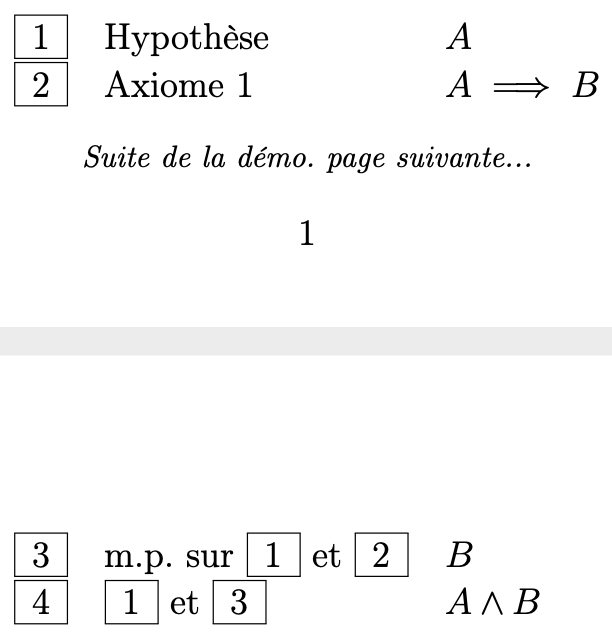
\includegraphics[scale = .5]{images/demo-explained-univ-broken[fr].png}}
\end{figure}
%\section{Détailler un \og vrai \fg{} raisonnement}

\subsection{Un tableau pour le collège et le lycée} \label{tnslog-tab-hard-proof-for-youngs}


\newparaexample{Avec les réglages par défaut}

L'environnement étoilé \env{demotab*} est différent de l'environnement \env{demotab} puisqu'il sert à indiquer trois choses et non juste deux comme le montre l'exemple suivant
\footnote{
	C'est pour cela qu'est proposé une version étoilée de l'environnement et non l'utilisation d'une option de l'environnement non étoilé. 
}.
Par contre, la syntaxe est très similaire.
Notez au passage la possibilité d'utiliser \macro{newline} pour forcer un retour à la ligne dans une cellule et aussi la nécessité d'écrire les accolades de la macro sans argument \macro{demostep} lorsque la 1\iere{} case est vide \emph{(ceci est inutile lorsque l'argument optionnel est renseigné comme nous allons le vérifier dans l'exemple juste après)}.

\begin{latexex-flat}
\begin{demotab*}
    \demostep
        $ABC$ est un triangle \newline équilatéral 
      & Définition d'un triangle \newline équilatéral. 
      & $AB = BC = AC$
    \demostep{} % --> Ne pas oublier ici !
      & Voir l'énoncé.
      & $AB = 10 \, cm$
    \demostep
        Voir les conséquences \newline \explref*{1} et \explref*{2} .
      & Simple calcul.
      & $ABC$ a pour périmètre $30 \, cm$.
\end{demotab*}
\end{latexex-flat}


% ---------------------- %


\newparaexample{Avec toutes les options}

Le système de référence marche ici aussi.
Par contre \env{demotab*} ne propose que \verb+start+ comme clé optionnelle avec le même fonctionnement que pour \env{demotab}.

\begin{latexex-flat}
\begin{demotab*}[start = last]
    \demostep[demo-first-geo-fact]
        $ABC$ est un triangle \newline équilatéral 
      & Définition d'un triangle \newline équilatéral. 
      & $AB = BC = AC$
    \demostep[known-data]
      & Voir l'énoncé.
      & $AB = 10 \, cm$
    \demostep
        Voir les conséquences \newline
        \explref{demo-first-geo-fact} et \explref{known-data} .
      & Simple calcul.
      & $ABC$ a pour périmètre $30 \, cm$.
\end{demotab*}
\end{latexex-flat}


% ---------------------- %


\subsection{Un tableau sur plusieurs pages}

Un tableau devant utiliser plusieurs pages sera scindé comme ci-dessous sans perte d'information
\footnote{
	Tout le travail est fait par l'environnement \env{longtable} du package éponyme.
}.

\begin{figure}[hbt!]
	\centering
	\frame{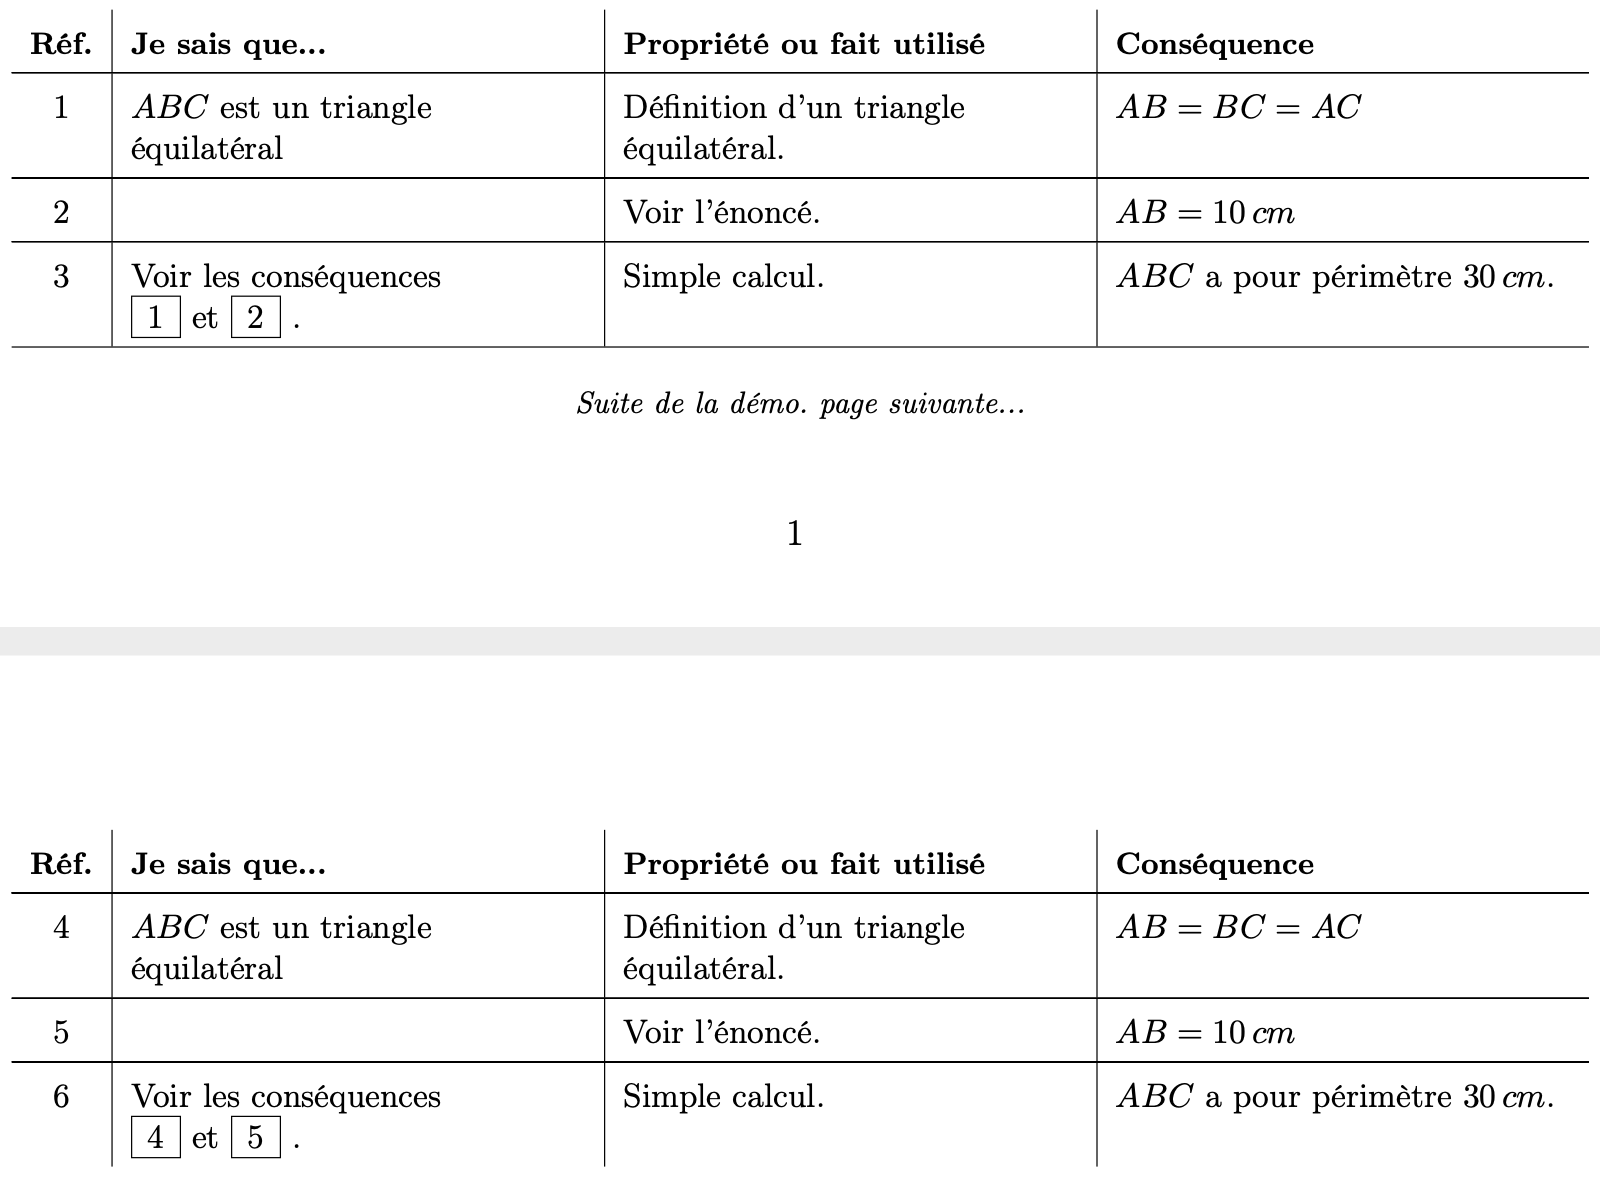
\includegraphics[scale = .5]{images/demotab-middleschool-broken[fr].png}}
\end{figure}
%\section{Détailler un raisonnement}
\chapter{Géométrie}

\section{Ensembles géométriques}

Se reporter à la section \ref{tnssets-geo-sets} page \pageref{tnssets-geo-sets} où est présentée la macro \macro{setgeo} pour indiquer des ensembles géométriques.
\section{Utiliser des unités S.I.}

Comme l'excellent package \verb#siunitx# est chargé en coulisse il devient facile de travailler avec des unités de mesure tout en respectant
\textbf{%
les conventions d'écriture qui seront françaises
	\footnote{
		Notez dans l'exemple l'écriture de $\num{1230}$ n'utilise pas d'espace contrairement à celle de $\num{12300}$.
	}
dès lors que vous aurez chargé \texttt{babel} avec l'option \texttt{french}%
} comme c'est le cas pour cette documentation.
Notez que les espaces dans \verb#\num{123 000}# et \verb#\num{1230 * 100}# sont inutiles mais qu'ils facilitent la relecture du code.

\begin{latexex}
$\ang{180} = \SI{\pi}{\radian}$ ,
$\SI{1}{km} = \SI{1e3}{m}$ avec aussi
$\num{123 000} = \num{1230 * 100}$
\end{latexex}
\section{Points et lignes}

\subsection{Points}

\newparaexample{Sans indice}

\begin{latexex}
$\pt{I}$
\end{latexex}


% ---------------------- %


\newparaexample{Avec un indice}

\begin{latexex}
$\pt*{I}{1}$ ou
$\pt*{I}{2}$
\end{latexex}


% ---------------------- %


\subsection{Lignes}

\newparaexample{Les droites}

Dans l'exemple suivant, le préfixe \prefix{g} est pour \whyprefix{g}{éometrie} tandis que \prefix{p} est pour \whyprefix{p}{oint}
\footnote{
	Comme la macro \macro{line} est proposée par \LaTeX, il a fallu ajouter le préfixe \texttt{g}.
}.

\begin{latexex}
$\gline{A}{B}$ ,
$\gline{\pt{A}}{\pt{B}}$ ou
$\gpline{A}{B}$
\end{latexex}


% ---------------------- %


\newparaexample{Les segments}

Les macros \macro{segment} et \macro{psegment} ont un comportement similaire à \macro{gline} et \macro{gpline}.

\begin{latexex}
$\segment{A}{B}$ ,
$\segment{\pt{A}}{\pt{B}}$ ou
$\psegment{A}{B}$
\end{latexex}


% ---------------------- %


\newparaexample{Les demi-droites}

Dans l'exemple suivant, le préfixe \prefix{h} est pour \whyprefix{h}{alf}  soit \inenglish{moitié}.

\begin{latexex}
$\ghline{A}{B}$ ,
$\ghline{\pt{A}}{\pt{B}}$ ou
$\gphline{A}{B}$
\end{latexex}


% ---------------------- %


\newparaexample{D'autres demi-droites}

Ce qui suit nécessite d'utiliser l'argument optionnel de \macro{gline} et \macro{gpline}. La valeur \prefix{OC} provient de \whyprefix{O}{pened} -- \whyprefix{C}{losed} soit \inenglish{ouvert -- fermé}.

\begin{latexex}
$\gline[OC]{A}{B}$ ,
$\gline[OC]{\pt{A}}{\pt{B}}$ ou
$\gpline[OC]{A}{B}$
\end{latexex}


\begin{remark}
	Les segments utilisent en fait l'option \prefix{C} et les demi-droites standard l'option \prefix{CO}.
	La valeur par défaut est \prefix{O}.
\end{remark}


% ---------------------- %


\subsection{Droites parallèles ou non}

Les opérateurs \macro{parallel} et \macro{nparallel} utilisent des obliques au lieu de barres verticales comme le montre l'exemple qui suit où \macro{stdnparallel} est un alias de \macro{nparallel} fourni par le package \verb+amssymb+, et \macro{stdparallel} est un alias de la version standard de \macro{parallel} proposée par \LaTeX{}.

\begin{latexex}
$\gpline{A}{B} \parallel \gpline{C}{D}$
au lieu de
$\gpline{A}{B}
 \stdparallel \gpline{C}{D}$

$\gpline{E}{F} \nparallel \gpline{G}{H}$
au lieu de
$\gpline{E}{F}
 \stdnparallel \gpline{G}{H}$
\end{latexex}


% ---------------------- %
\section{Vecteurs}

\subsection{Les écrire}

\newparaexample{}

\begin{latexex}
$\vect{UnNomLong}$  ,
$\vect*{e}{rot}$ ou
$\vect{e_{rot}}$
\end{latexex}


% ---------------------- %


\newparaexample{Sans point disgracieux}

\begin{latexex}
$\vect{i}$ ou
$\vect*{j}{2}$
\end{latexex}


% ---------------------- %


\newparaexample{Se passer de la macro \macro{pt}}

\begin{latexex}
$\pvect{A}{B} = \vect{\pt{A}\pt{B}}$. 
\end{latexex}


% ---------------------- %
% \section{Vecteurs}

\subsection{Norme}

\begin{latexex}
 $\norm{\vect{i}} = \vnorm{i}$

 $\norm {\dfrac{2}{7} \vect*{e}{k}}
= \norm*{\dfrac{2}{7} \vect*{e}{k}}$
\end{latexex}


\begin{remark}
	Le code \LaTeX{} pour des doubles barres extensibles ou non vient directement de ce message : \url{https://tex.stackexchange.com/a/43009/6880}.
\end{remark}


% ---------------------- %
%\section{Vecteurs}

\subsection{Produit scalaire}

Les 1\iers{} exemples utilisent une syntaxe longue mais adaptables à toutes les situations.
Voir l'exemple \ref{tnsgeo-long-dot-prod} un peu plus bas pour une écriture rapide utilisable dans certains cas.


% ---------------------- %


\newparaexample{Version classique}

\begin{latexex}
$\dotprod{\dfrac{1}{2} \vect{u}}%
         {\vect{v}}$
\end{latexex}


% ---------------------- %


\newparaexample{Version \og pédagogique mais pas écolo. \fg}

Dans l'exemple suivant l'option \prefix{b} est pour \whyprefix{b}{ullet} soit \inenglish{puce}.
Cette écriture peut être utile avec des débutants mais elle est peu pratique pour une écriture manuscrite.

\begin{latexex}
$\dotprod[b]{\dfrac{1}{2} \vect{u}}%
            {\vect{v}}$
\end{latexex}


% ---------------------- %


\newparaexample{Écriture \og universitaire \fg}

Dans l'exemple suivant l'option \prefix{p} est pour \whyprefix{p}{arenthèse} et dans \prefix{sp} le \prefix{s} est pour \whyprefix{s}{mall} soit \inenglish{petit}. On rencontre souvent cette écriture dans les cursus mathématiques universitaires.

\begin{latexex}
$\dotprod[p]{\dfrac{1}{2} \vect{u}}%
            {\vect{v}}$

$\dotprod[sp]{\dfrac{1}{2} \vect{u}}%
             {\vect{v}}$
\end{latexex}


% ---------------------- %


\newparaexample{Écriture \og à la physicienne \fg}

Dans l'exemple suivant \prefix{r} est pour \whyprefix{r}{after} soit \inenglish{chevron}. Les physiciens aiment bien cette notation.

\begin{latexex}
$\dotprod[r]{\dfrac{1}{2} \vect{u}}%
            {\vect{v}}$

$\dotprod[sr]{\dfrac{1}{2} \vect{u}}%
             {\vect{v}}$
\end{latexex}


% ---------------------- %


\newparaexample{Version courte mais restrictive} \label{tnsgeo-long-dot-prod}

Dans l'exemple suivant le préfixe \prefix{v} est pour \whyprefix{v}{ecteur}.
Notons que dans ce cas les options \prefix{sp} et \prefix{sr} n'apportent rien de nouveau.

\begin{latexex}
 $\vdotprod   {u}{v}
= \vdotprod[b]{u}{v}$
 
 $\vdotprod[r]{u}{v}
= \vdotprod[p]{u}{v}$
\end{latexex}


% ---------------------- %

%
%\newparaexample{Écriture formelle développée}
%
%Ce qui suit peut rendre service... ou pas.
%Dans l'exemple ci-dessous \prefix{exp} est pour \whyprefix{exp}{and} c'est à dire \inenglish{développer}, \prefix{c} pour \macro{cdot} et enfin \prefix{t} pour \macro{times}.
%
%\begin{latexex}
%$\dotprod[exp]{\vect{u}}{\vect{v}}$
%
%$\vdotprod[cexp]{u}{v}$
%
%$\vdotprod[texp]{u}{v}$
%\end{latexex}


% ---------------------- %
%\section{Vecteurs}

\subsection{3D -- Produit vectoriel}

\subsubsection{Écriture symbolique}

\newparaexample{Version classique en France}

\begin{latexex}
$\crossprod{\dfrac{1}{2} \vect{i}}%
           {\vect{j}}$ 
\end{latexex}


% ---------------------- %


\newparaexample{Version alternative}

La macro \macro{crossprod} possède un argument optionnel que l'on peut utiliser pour obtenir la mise en forme suivante.

\begin{latexex}
$\crossprod[t]{\dfrac{1}{2} \vect{i}}%
              {\vect{j}}$ 
\end{latexex}


% ---------------------- %


\newparaexample{Version courte mais restrictive}

\begin{latexex}
$\vcrossprod   {i}{j}$ ou
$\vcrossprod[t]{i}{j}$
\end{latexex}


% ---------------------- %


\subsubsection{Explication du mode de calcul}

\newparaexample{}

Dans l'exemple suivant, le préfixe \prefix{calc} est pour \whyprefix{calc}{uler} quant à \prefix{v} est pour \whyprefix{v}{ecteur} pour une rédaction raccourcie pour les vecteurs.

\begin{latexex}
$\calccrossprod{\vect{u}}{x}{y}{z}%
               {\vect{v}}{x'}{y'}{z'}$
ou
$\vcalccrossprod{AB}{x_B - x_A}%
                    {y_B - y_A}%
                    {z_B - z_A}%
                {CD}{x_D - x_C}%
                    {y_D - y_C}%
                    {z_D - z_C}$
\end{latexex}


\begin{remark}
    Tous les exemples suivants se feront avec \macro{vcalccrossprod} mais bien entendu ils restent adaptables directement à \macro{calccrossprod}.
\end{remark}


% ---------------------- %


\newparaexample{Pour un public averti}

On peut juste proposer des croix fléchées ou non, voir juste les coordonnées \og augmentées \fg{} sans les décorations comme ci-après via l'argument optionnel de \macro{calccrossprod} ou \macro{vcalccrossprod}.

\begin{latexex}
$ \vcalccrossprod[arrows]{u}{x}{y}{z}%
                         {v}{x'}{y'}{z'}
= \vcalccrossprod[cross] {u}{x}{y}{z}%
                         {v}{x'}{y'}{z'}
= \vcalccrossprod[nodeco]{u}{x}{y}{z}%
                         {v}{x'}{y'}{z'}$
\end{latexex}


% ---------------------- %


\newparaexample{Sans les vecteurs}

Si les vecteurs vous gênent il suffira d'utiliser l'option \verb+novec+ pour \verb+no+ \whyprefix{vec}{tor} soit \inenglish{pas de vecteur}.
Voici deux cas d'utilisation
\footnote{
	Il peut sembler un peu lourd d'avoir des arguments pour des vecteurs non affichés mais ce choix permet à l'usage de faire des copier-coller redoutables d'efficacité !
}.


\begin{latexex}
$ \vcalccrossprod[novec]
      {u}{x}{y}{z}{v}{x'}{y'}{z'}
= \vcalccrossprod[novec,cross]
      {u}{x}{y}{z}{v}{x'}{y'}{z'}$
\end{latexex}



% ---------------------- %


\newparaexample{Les coordonnées \og développées \fg}

Parmi les options proposées par \macro{calccrossprod} et \macro{vcalccrossprod}, il y en existe quelques unes fournissant des coordonnées
\footnote{
	En coulisse on utilise la macro \macro{coord} présentée dans la section \ref{tnsgeo-coordinates} page \pageref{tnsgeo-coordinates} dont on reprend les options de mise en forme. 
}
détaillant les calculs. Indiquons que \prefix{exp} est pour \whyprefix{exp}{and} soit \inenglish{développer}, \prefix{c} pour \macro{cdot} et enfin \prefix{t} pour \macro{times}
\footnote{
	De nouveau on obtient ici une méthode très pratique à l'usage car elle permet de faire des copier-coller.
}.


\begin{latexex}
$\vcalccrossprod[exp]%
                {u}{\dfrac{1}{2}x}{y}{z}%
                {v}{x'}{y'}{z'}$

$\vcalccrossprod[cexp,vb]%
                {u}{\dfrac{1}{2}x}{y}{z}%
                {v}{x'}{y'}{z'}$

$\vcalccrossprod[texp,sp]%
                {u}{\dfrac{1}{2}x}{y}{z}%
                {v}{x'}{y'}{z'}$
\end{latexex}


\medskip


Voici les options disponibles. Nous expliquons ensuite comment les utiliser.
\begin{enumerate}
	\item \prefix{p} vient de \whyprefix{p}{arenthèses}. Ceci donnera une écriture horizontale.

	\item \prefix{b} vient de \whyprefix{b}{rackets} soit \inenglish{crochets}. Ceci donnera une écriture horizontale.

	\item \prefix{sp} et \prefix{sb} produisent des délimiteurs non extensibles en mode horizontal.
	      Ici \prefix{s} vient de \whyprefix{s}{mall} soit \inenglish{petit}.

	\item \prefix{vp} et \prefix{vb} produisent des écritures verticales.
	      Ici \prefix{v} vient de \whyprefix{v}{ertical}.

	\medskip

	\item \prefix{exp} tout seul demande d'utiliser un espace pour séparer les facteurs de chaque produit.

	\item \prefix{texp} tout seul demande d'utiliser \macro{times} comme opérateur de multiplication.

	\item \prefix{cexp} tout seul demande d'utiliser \macro{cdot} comme opérateur de multiplication.
\end{enumerate}

\bigskip


\textbf{Attention !}
Les produits sont rédigés stupidement. Autrement dit ce sera à vous d'ajouter des parenthèses là où il y en aura besoin sinon vous obtiendrez des horreurs comme celle ci-dessous.
    
\begin{latexex}
$\vcalccrossprod[exp,vb]%
 {AB}%
 {x_B - x_A}{y_B - y_A}{z_B - z_A}%
 {CD}%
 {x_D - x_C}{y_D - y_C}{z_D - z_C}$
\end{latexex}

Ici nous n'avons pas d'autre choix que de corriger le tir nous-même.
Ceci étant indiqué, ce genre de situation est très rare dans la vraie vie mathématique où l'on évite d'avoir à calculer un produit vectoriel avec des expressions compliquées.
    
\begin{latexex}
$\vcalccrossprod[exp,vb]%
 {AB}%
 {(x_B - x_A)}{(y_B - y_A)}{(z_B - z_A)}%
 {CD}%
 {(x_D - x_C)}{(y_D - y_C)}{(z_D - z_C)}$
\end{latexex}


% ---------------------- %
%\section{Vecteurs}

\subsection{2D -- Déterminant de deux vecteurs}

\newparaexample{Version décorée avec une boucle}

Dans l'exemple suivant, le préfixe \prefix{calc} est pour \whyprefix{calc}{uler} quant à \prefix{v} est pour \whyprefix{v}{ecteur} pour une rédaction raccourcie pour les vecteurs.

\begin{latexex}
$\calcdetplane{\vect{u}}{x}{y}%
              {\vect{v}}{x'}{y'}$
ou
$\vcalcdetplane{AB}%
               {x_B - x_A}{y_B - y_A}%
               {CD}%
               {x_D - x_C}{y_D - y_C}$
\end{latexex}


\begin{remark}
    Tous les exemples suivants se feront avec \macro{vcalcdetplane} mais bien entendu ils restent adaptables directement à \macro{calcdetplane}.
\end{remark}


% ---------------------- %


\newparaexample{Version décorée avec une croix fléchée}

L'argument optionnel de \macro{calcdetplane} ou \macro{vcalcdetplane} permet d'obtenir une croix fléchée au lieu d'une boucle.

\begin{latexex}
$\vcalcdetplane[arrows]{u}{x}{y}%
                       {v}{x'}{y'}$
\end{latexex}


% ---------------------- %


\newparaexample{Version décorée avec une croix non fléchée}

\begin{latexex}
$\vcalcdetplane[cross]{u}{x}{y}%
                      {v}{x'}{y'}$
\end{latexex}


% ---------------------- %


\newparaexample{Version non décorée}

\begin{latexex}
$\vcalcdetplane[nodeco]{u}{x}{y}%
                       {v}{x'}{y'}$
\end{latexex}


% ---------------------- %


\newparaexample{Sans les vecteurs}

\begin{latexex}
 $\vcalcdetplane[novec]%
                {u}{x}{y} {v}{x'}{y'}
= \vcalcdetplane[novec,cross]%
                {u}{x}{y} {v}{x'}{y'}$
\end{latexex}


\newparaexample{Calcul développé}

Grâce à l'argument optionnel de \macro{calcdetplane} ou de \macro{vcalcdetplane} il est aussi possible d'obtenir le résultat développé du calcul comme ci-après
où \prefix{exp} est pour \whyprefix{exp}{and} soit \inenglish{développer}, \prefix{c} pour \macro{cdot} et enfin \prefix{t} pour \macro{times}
\footnote{
	Même si les vecteurs ne sont pas utilisés pour la mise en forme, on obtient ici une méthode très pratique à l'usage car elle permet de faire des copier-coller.
}.

\begin{latexex}
$\vcalcdetplane[exp]{u}{x}{y}%
                    {v}{x'}{y'}$

$\vcalcdetplane[cexp]{u}{x}{y}%
                     {v}{x'}{y'}$

$\vcalcdetplane[texp]{u}{x}{y}%
                     {v}{x'}{y'}$
\end{latexex}


\textbf{Attention !}
Le développement effectué est stupide. Autrement dit ce sera à vous d'ajouter des parenthèses là où il y en aura besoin sinon vous obtiendrez des horreurs comme celle qui suit.
    
\begin{latexex}
$\vcalcdetplane[exp]{AB}%
                    {x_B - x_A}%
                    {y_B - y_A}%
                    {CD}%
                    {x_D - x_C}%
                    {y_D - y_C}$
\end{latexex}

Ici nous n'avons pas d'autre choix que de régler le problème à la main. Ce genre de situation n'est pas rare dans la vraie vie mathématique.
    
\begin{latexex}
$\vcalcdetplane[exp]{AB}%
                    {(x_B - x_A)}%
                    {(y_B - y_A)}%
                    {CD}%
                    {(x_D - x_C)}%
                    {(y_D - y_C)}$
\end{latexex}


% ---------------------- %
\section{Géométrie cartésienne}

\subsection{Coordonnées} \label{tnsgeo-coordinates}

\newparaexample{Des coordonnées seules}

\verb+tnsgeo+ propose, via un argument optionnel, six façons différentes de rédiger des coordonnées seules \emph{(nous verrons après des macros pour les coordonnées d'un point et celles d'un vecteur afin de produire un code \LaTeX{} plus sémantique)}. Commençons par les écritures horizontales où vous noterez l'utilisation de \verb+|+ pour séparer les coordonnées dont le nombre peut être quelconque.

\begin{latexex}
$\coord    {\dfrac{1}{3} | -4 | 0}$ ou
$\coord[sp]{\dfrac{1}{3} | -4 | 0}$

$\coord[b] {\dfrac{1}{3} | -4 | 0}$ ou
$\coord[sb]{\dfrac{1}{3} | -4 | 0}$
\end{latexex}


Il existe en plus deux versions verticales.

\begin{latexex}
$\coord[vp]{3 | -4}$ ou
$\coord[vb]{3 | -4}$
\end{latexex}


Voici d'où viennent les noms des options.
\begin{enumerate}
	\item \prefix{p}, qui est aussi la valeur par défaut, vient de \whyprefix{p}{arenthèses}.

	\item \prefix{b} vient de \whyprefix{b}{rackets} soit \inenglish{crochets}.

	\item \prefix{s} pour \whyprefix{s}{mall} soit \inenglish{petit} permet d'avoir des délimiteurs non extensibles en mode horizontal car par défaut ils le sont.

	\item \prefix{v} pour \whyprefix{v}{ertical} demande de produire une écriture verticale.
\end{enumerate}


% ---------------------- %


\newparaexample{Coordonnées d'un point}

La macro \macro{pcoord} avec \prefix{p} pour  \whyprefix{p}{oint} prend un argument supplémentaire avant les coordonnées qui est le nom d'un point qui sera mis en forme par la macro \macro{pt}. Si vous ne souhaitez pas que \macro{pt} soit appliquée, il suffit de passer via la version étoilée \macro{pcoord*}.

\begin{latexex}
$\pcoord{A}{3 | -4 | 0 | -1}$ ou
$\pcoord*{\Sigma}{7 | 9 | 8}$
\end{latexex}


Toutes les options disponibles avec \macro{coord} le sont aussi avec  \macro{pcoord}. 

\begin{latexex}
$\pcoord[b]{A}{3 | -4 | 0 | -1}$ ou
$\pcoord*[b]{\Sigma}{7 | 9 | 8}$
\end{latexex}



% ---------------------- %


\newparaexample{Coordonnées d'un vecteur}

Le fonctionnement de \macro{vcoord} est similaire à celui de \macro{pcoord} si ce n'est que c'est la macro \macro{vect} qui sera appliquée si besoin.

\begin{latexex}
$\vcoord{u}{3 | -4}$ ou
$\vcoord*{\dfrac{1}{2} \vect{u}}%
         {3 | -4}$

$\vcoord[vp]{u}{3 | -4}$ ou
$\vcoord*[vp]{\dfrac{1}{2} \vect{u}}%
             {3 | -4}$
\end{latexex}


% ---------------------- %
% \section{Géométrie cartésienne}

\subsection{Nommer un repère}

\newparaexample{La méthode basique}

Commençons par la manière la plus basique d'écrire un repère \textit{(nous verrons d'autres méthodes qui peuvent être plus efficaces)}.

\begin{latexex}
$\axes{\pt{O} %
     | \pt{I} | \pt{J}}$
\end{latexex}


% ---------------------- %


\newparaexample{La méthode basique en version étoilée}

Dans l'exemple ci-dessous, on voit que la version étoilée produit des petites parenthèses.
\begin{latexex}
$\axes{\pt{O} %
     | \dfrac{7}{3} \vect{i} %
     | \vect{j}}$
ou
$\axes*{\pt{O} %
     | \dfrac{7}{3} \vect{i} %
     | \vect{j}}$
\end{latexex}


% ---------------------- %


\newparaexample{La méthode basique en dimension quelconque}

Il faut au minimum deux "morceaux" séparés par des barres \verb+|+, cas de la dimension $1$, mais il n'y a pas de maximum, cas d'une dimension quelconque $n > 0$.

\begin{latexex}
$\axes{\pt{O} %
     | \vect*{i}{1} %
     | \vect*{i}{2} %
     | \vect*{i}{3} %
     | \dots %
     | \vect*{i}{9} %
     | \vect*{i}{10} %
     | \vect*{i}{11} %
     | \vect*{i}{12}}$
\end{latexex}


% ---------------------- %


\newparaexample{Repère affine}

Dans l'exemple suivant, le préfixe \prefix{p} est pour \whyprefix{p}{oint}.

\begin{latexex}
$\paxes{O | I | J | K}$
au lieu de
$\axes{\pt{O} %
     | \pt{I} | \pt{J} | \pt{K}}$
\end{latexex}


% ---------------------- %


\newparaexample{Repère vectoriel (méthode 1)}

Dans l'exemple suivant, le préfixe \prefix{v} est pour \whyprefix{v}{ecteur}.

\begin{latexex}
$\vaxes{\pt{O} | i | j}$
au lieu de
$\axes{\pt{O} | \vect{i} | \vect{j}}$
\end{latexex}


% ---------------------- %


\newparaexample{Repère vectoriel (méthode 2)}

Dans l'exemple suivant, le préfixe \prefix{pv} permet de combiner ensemble les fonctionnalités proposées par les préfixes \prefix{p} et \prefix{v}.

\begin{latexex}
$\pvaxes{O | i | j}$
au lieu de
$\axes{\pt{O} | \vect{i} | \vect{j}}$
\end{latexex}


% ---------------------- %
% \section{Géométrie}

\section{Arcs circulaires}

\newparaexample{}

L'arc extensible utilise une macro que l'on trouve dans le package \verb#yhmath#.

\begin{latexex}
$\circarc{UnNomLong}$ ,
$\circarc*{A}{rot}$ ou
$\circarc{A_{rot}}$
\end{latexex}


% ---------------------- %


\newparaexample{}

\begin{latexex}
$\circarc{i}$ ou
$\circarc*{j}{2}$
\end{latexex}


% ---------------------- %
% \section{Géométrie}

\section{Angles}

\subsection{Angles géométriques \og intérieurs \fg}

\newparaexample{}

Le chapeau extensible utilise une macro que l'on trouve dans le package \verb#yhmath#.

\begin{latexex}
$\anglein{UnNomLong}$ ,
$\anglein*{A}{rot}$ ou
$\anglein{A_{rot}}$
\end{latexex}


% ---------------------- %


\newparaexample{Cacher les points du i et du j}

\begin{latexex}
$\anglein{i}$ ou
$\anglein*{j}{2}$
\end{latexex}


% ---------------------- %
% \section{Géométrie}

%\section{Angles}

\subsection{Angles orientés de vecteurs}

\paragraph{Sans chapeau - Version longue}

L'option par défaut est \prefix{p} pour \whyprefix{p}{arenthèse}.
Dans \prefix{sp} le \prefix{s} est pour \whyprefix{s}{mall} soit \inenglish{petit}.
 
\begin{latexex}
$\angleorient    {\dfrac{1}{2} \vect{i}}%
                 {\vect{j}}$

$\angleorient[sp]{\dfrac{1}{2} \vect{i}}%
                 {\vect{j}}$
\end{latexex}


% ---------------------- %


\paragraph{Sans chapeau - Version courte mais restrictive}

Dans l'exemple suivant, le préfixe \prefix{v} est pour \whyprefix{v}{ecteur} qui permet de simplifier la saisie quand l'on a juste des vecteurs nommés avec des lettres
\emph{(notez que l'option \prefix{sp} n'apporte rien de nouveau)}.

\begin{latexex}
$\vangleorient    {i}{j}$ comme
$\vangleorient[sp]{i}{j}$
\end{latexex}


% ---------------------- %


\paragraph{Avec un chapeau}

Dans l'exemple suivant, \prefix{h} est pour \whyprefix{h}{at} soit \inenglish{chapeau}.
Notez au passage que \prefix{sh} produit juste des parenthèses petites mais ce choix de nom simplifie l'utilisation de la macro \emph{(c'est mieux que \prefix{hsp} par exemple)}.

\begin{latexex}
$\angleorient[h] {\dfrac{1}{2} \vect{i}}%
                 {\vect{j}}$

$\angleorient[sh]{\dfrac{1}{2} \vect{i}}%
                 {\vect{j}}$

$\vangleorient[h] {i}{j}$ comme
$\vangleorient[sh]{i}{j}$
\end{latexex}


% ---------------------- %
\chapter{Analyse}

\section{Constantes et paramètres}

\subsection{Constantes classiques ajoutées}

\newparaexample{}

Les macros ci-dessous ne nécessitent pas d'accolades.

% List of classical constants - START

\begin{latexex}
$\ggamma$ , $\ppi$ , $\ttau$ ,
$\ee$ , $\ii$ , $\jj$ 
et $\kk$ où $\ttau = 2 \ppi$
\end{latexex}

% List of classical constants - END


\begin{remark}
	Faites attention car \verb+{\Large $\ppi \neq \pi$}+ produit {\Large $\ppi \neq \pi$}. Comme vous le constatez, les symboles ne sont pas identiques. Ceci est vraie pour toutes les constantes grecques.
\end{remark}


% ---------------------- %


\newparaexample{Gestion de l'espace}

Le choix a été fait d'ajouter de l'espace autour des constantes ajoutées.

\begin{latexex}
$2 \ppi R$ ou $2 \pi R$
\end{latexex}


% ---------------------- %


\subsection{Constantes latines personnelles}

La macro \macro{param} est surtout là pour une utilisation pédagogique. Noter au passage qu'ici aussi un espace est ajouté autour des paramètres.

\begin{latexex}
$\param{a} x^2 + \param{b} x + \param{c}$
ou
$a x^2 + b x + c$
\end{latexex}


% ---------------------- %
\section{Une variable \og symbolique \fg{}}

Le package \verb+tnscom+, chargé en coulisse, propose la macro \macro{symvar} qui produit différents symboles donnés ci-dessous.

\begin{latexex}
$\symvar = \symvar[1]$ ou $\symvar[2]$

$\symvar[3]$ ou $\symvar[4]$
\end{latexex}

Le nom \prefix{symvar} vient de \whyprefix{symb}{olic} \whyprefix{var}{iable} soit \inenglish{variable symbolique}.
Ces symboles sont utiles pour indiquer un argument symboliquement sans faire référence précisément à une ou des variables nommées.


% ---------------------- %
\section{La fonction valeur absolue}

\newparaexample*{}

\begin{latexex}
$\abs{2}$ ,
$\abs {\dfrac{3}{5}}$ ou
$\abs*{\dfrac{3}{5}}$
\end{latexex}


\begin{remark}
	Le code \LaTeX{} vient directement de ce poste : \url{https://tex.stackexchange.com/a/43009/6880}.
\end{remark}


% ---------------------- %
\section{Fonctions nommées spéciales}

\subsection{Sans paramètre}

Quelques fonctions nommées ont été ajoutées en plus de celles fournies par le package \verb#amsmath#  qui est chargé en coulisse et propose par exemple $\lg x$ et $\ln x$ via les macros \macro{lg} et \macro{ln}.
Ci-dessous le \prefix{f} dans \prefix{fch} est pour \whyprefix{f}{rench} soit \inenglish{français} \emph{(ce choix sert à éviter des incompatibilités avec d'autres packages)}. La liste complète des fonctions nommées est donnée plus bas dans la section  \ref{tnsana-all-named-functions}

\begin{latexex}
$\fch x = \cosh x$ ou $\acos x$
\end{latexex}


% ---------------------- %


\subsection{Avec un paramètre}

Voici des fonctions utilisables avec un paramètre optionnel.

\begin{latexex}
$\exp[6] y = 6^y$   ,
$\log[2] x = \lg x$ ,
$\lg[3] x$ et $\ln[4] x$
\end{latexex}


% ---------------------- %


\subsection{Toutes les fonctions nommées en plus} \label{tnsana-all-named-functions}

\vspace{-1em}

% Table of all - START
\begin{longtable}{p{0.3\linewidth}p{0.3\linewidth}p{0.3\linewidth}}
\verb#\acos x   # : $\acos x   $ & \verb#\asin x   # : $\asin x   $ & \verb#\atan x   # : $\atan x   $
\\[.75ex]
\verb#\arccosh x# : $\arccosh x$ & \verb#\arcsinh x# : $\arcsinh x$ & \verb#\arctanh x# : $\arctanh x$
\\[.75ex]
\verb#\acosh x  # : $\acosh x  $ & \verb#\asinh x  # : $\asinh x  $ & \verb#\atanh x  # : $\atanh x  $
\\[.75ex]
\verb#\fch x    # : $\fch x    $ & \verb#\fsh x    # : $\fsh x    $ & \verb#\fth x    # : $\fth x    $
\\[.75ex]
\verb#\afch x   # : $\afch x   $ & \verb#\afsh x   # : $\afsh x   $ & \verb#\afth x   # : $\afth x   $
\\[.75ex]
\verb#\exp x    # : $\exp x    $ & \verb#\exp[p] x # : $\exp[p] x $ & 
\\[.75ex]
\verb#\lg x     # : $\lg x     $ & \verb#\lg[p] x  # : $\lg[p] x  $ & 
\\[.75ex]
\verb#\ln x     # : $\ln x     $ & \verb#\ln[p] x  # : $\ln[p] x  $ & 
\\[.75ex]
\verb#\log x    # : $\log x    $ & \verb#\log[p] x # : $\log[p] x $ & 
\end{longtable}
% Table of all - END
\section{Limite}

\newparaexample{Cas minimaliste}

Notez ci-dessous que le rendu de la limite via \macro{limit} se fait toujours en mode \macro{displaystyle} pour l'opérateur de limite.

\begin{latexex}
$\limit{f(x)}{x}{0} = \frac{1}{2}$
\end{latexex}


\begin{remark}
	\verb#\lim\limits_{x \rightarrow 0} f(x)# produit 
	$\lim\limits_{x \rightarrow 0} f(x)$ contre 
	$\limit{f(x)}{x}{0}$ ci-dessus.
	La version \macro{limit} utilise un petit peu plus d'espace sous le mot lim.
\end{remark}



% ---------------------- %


\newparaexample{Avec des conditions}

Ce 2\ieme{} exemple devrait rendre intéressante la macro \macro{limit} qui permet d'ajouter facilement plusieurs conditions
\footnote{
	En pratique, on utilise généralement au maximum une condition.
}
comme le montre la 2\ieme{} limite ci-après.

\begin{latexex}
$\limit{f(x)}{x}{0 | x > 0}$ ou
$\limit{f(z)}{z}%
       {0 | z \in \Omega | \abs{z} < 3}$
\end{latexex}


% ---------------------- %


\newparaexample{Ajout de parenthèses}

Les options \verb#p# et \verb#sp# permettent d'ajouter facilement des parenthèses extensibles ou non autour de la fonction. 
Indiquons que \prefix{sp} est pour \whyprefix{s}{mall} \whyprefix{p}{arenthesis} soit \inenglish{petites parenthèses}.

\begin{latexex}
$\limit[p] {\dfrac{1}{x}}{x}%
           {0 | x > 0}$
ou
$\limit[sp]{\dfrac{1}{x}}{x}%
           {0 | x > 0}$
\end{latexex}


% ---------------------- %
\section{Calcul différentiel}

\subsection{\texorpdfstring{Les opérateurs $\pp{}$ et $\dd{}$}%                           {Les opérateurs "d rond" et "d droit"}}
                           {Les opérateurs "d rond" et "d droit"}}

Voici deux opérateurs utiles aussi bien pour du calcul différentiel que du calcul intégral. 

\begin{latexex}
$\dd{t} = \dd[1]{t}$ ou $\dd[n]{x}$

$\pp{t} = \pp[1]{t}$ ou $\pp[n]{x}$
\end{latexex}


% ---------------------- %


\subsection{Dérivations totales d'une fonction -- Version longue avec une variable}

\newparaexample{Différentes écritures possibles}

La macro \macro{der} est stricte du point de vue sémantique car on doit lui fournir la fonction, l'ordre de dérivation et la variable de dérivation
\emph{(voir la section \ref{tnsana-short-der} qui présente la macro \macro{sder} permettant une rédaction efficace pour obtenir $\sder[e]{f}{1}$ ou $\sder{f}{1}$)}.
Voici plusieurs mises en forme faciles à taper via l'option de \macro{der}.
Attention bien entendu à n'utiliser l'option par défaut \prefix{u} ou l'option \prefix{d} qu'avec un ordre de dérivation de valeur naturelle connue !

\begin{latexex}
 $\der   {f}{x}{3}
= \der[e]{f}{x}{3}
= \der[d]{f}{x}{3}$

 $\der[i] {u}{x}{k}
= \der[f] {u}{x}{k}
= \der[sf]{u}{x}{k}$
\end{latexex}


On peut aussi ajouter autour de la fonction des parenthèses extensibles ou non sauf même si cela n'est pas utile pour le mode \prefix{d} \emph{(voir juste après le mode \prefix{bd})}.
Ci-dessous on montre au passage une écriture du type \emph{\og opérateur fonctionnel \fg} : voir la section \ref{tnsana-ope-total-der} page \pageref{tnsana-ope-total-der} à ce sujet.

\begin{latexex}
 $\der[osf,sp]{\frac{1}{2}  uv}{x}{k}
= \der[of,p]  {\dfrac{1}{2} uv}{x}{k}$
\end{latexex}


Avec l'option \prefix{d} les parenthèses seules sont sans utilité car on peut obtenir des choses non souhaitées comme $\der[d, p]{u + v}{x}{2}$.
À la place on utilisera l'option \prefix{bd} où le \prefix{b} est pour \whyprefix{b}{racket} soit \inenglish{crochet}. Notez au passage que \prefix{p} et \prefix{sp} restent utilisables.

\begin{latexex}
 $\der[bd]   {\frac{1}{2}  uv}{x}{2}
= \der[bd,p] {\frac{1}{2}  uv}{x}{2}
= \der[bd,sp]{\dfrac{1}{2} uv}{x}{2}$
\end{latexex}


\begin{remark}
	Expliquons les valeurs des options.
	\begin{enumerate}
		\item \prefix{u}, la valeur par défaut, est pour \whyprefix{u}{suel} soit l'écriture avec les primes. Cette option ne marchera pas avec un nombre symbolique de dérivations. 

		\item \prefix{e} est pour \whyprefix{e}{xposant}.

		\item \prefix{i} est pour \whyprefix{i}{ndice}.

		\item \prefix{d} est pour \whyprefix{d}{ot} soit \inenglish{point}.

		\item \prefix{bd} est pour \whyprefix{b}{racket} \whyprefix{d}{ot} où \inenglish*{bracket} est pour \inenglish{crochet}.

		\medskip
		
		\item \prefix{f} est pour \whyprefix{f}{raction} avec aussi \prefix{sf} pour une écriture réduite où \prefix{s} est pour \whyprefix{s}{mall} soit \inenglish{petit}.

		\item \prefix{of} et \prefix{osf} utilisent le préfixe \prefix{o} pour \whyprefix{o}{pérateur}.
		
		\medskip
		
		\item \prefix{p} est pour \whyprefix{p}{arenthèse} : dans ce cas les parenthèses seront extensibles. Le fonctionnement est différent avec l'option \prefix{d} comme nous l'avons vu avant.

		\item \prefix{sp} est pour des parenthèses non extensibles. Là aussi le fonctionnement est différent avec l'option \prefix{d}.
	\end{enumerate}
\end{remark}


% ---------------------- %


\newparaexample{Pas de uns inutiles}

\begin{latexex}
 $\der[i ]{u}{x}{1}
= \der[f ]{u}{x}{1}
= \der[sf]{u}{x}{1}
= \der[of]{u}{x}{1}$
\end{latexex}


\begin{remark}
	Voici comment forcer les exposants $1$ si besoin. Fonctionnel mais très moche...

	\begin{latexex}
 $\der[i ]{u}{x}{\,\!1}
= \der[f ]{u}{x}{\,\!1}
= \der[sf]{u}{x}{\,\!1}
= \der[of]{u}{x}{\,\!1}$
\end{latexex}
\end{remark}

% ---------------------- %


\subsection{Dérivations totales d'une fonction -- Version courte sans variable} \label{tnsana-short-der}

Dans l'exemple suivant le code manque de sémantique car on n'indique pas la variable de dérivation.
Ceci étant dit à l'usage la macro \macro{sder} rend de grands services.
Ici le préfixe \prefix{s} est pour \whyprefix{s}{imple} voire \whyprefix{s}{impliste}...
Voici des exemples où de nouveau l'option par défaut \prefix{u} et l'option \prefix{d} ne seront fonctionnelles qu'avec un ordre de dérivation de valeur naturelle connue !


\newparaexample{}

\begin{latexex}
 $\sder{f}{1} = \der{f}{x}{1}$

 $\sder   {f}{3}
= \sder[e]{f}{3}
= \sder[d]{f}{3}$
\end{latexex}


\newparaexample{}

\begin{latexex}
 $\sder[sp] {\dfrac{1}{2} uv}{2}
= \sder[e,p]{\dfrac{1}{2} uv}{2}
= \sder[bd] {\dfrac{1}{2} uv}{2}$
\end{latexex}


\begin{remark}
	Ici les seules options disponibles sont \prefix{u}, \prefix{e}, \prefix{b}, \prefix{bd}, \prefix{p} et \prefix{sp}.
\end{remark}


% ---------------------- %


\subsection{L'opérateur de dérivation totale} \label{tnsana-ope-total-der}

Ce qui suit peut rendre service au niveau universitaire.
Les options possibles sont \verb+f+, valeur par défaut, \verb+sf+ et \verb+i+ avec les mêmes significations que pour la macro \macro{der}.

\begin{latexex}
 $\derope    {x}{k}
= \derope[sf]{x}{k}
= \derope[i] {x}{k}$
\end{latexex}


Ici non plus il n'y a pas de uns inutiles mais l'astuce \verb+\,\!1+ reste utilisable.

\begin{latexex}
 $\derope    {x}{1}
= \derope[sf]{x}{1}
= \derope[i] {x}{1}$
\end{latexex}


% ---------------------- %
%\section{Calcul différentiel}

\subsection{Dérivations partielles}

\newparaexample{Différentes écritures}

La macro \macro{pder}
\footnote{
	\macro{partial} existe déjà pour obtenir $\partial$.
}
avec \prefix{p} pour \whyprefix{p}{artielle}
permet de rédiger des dérivées partielles en utilisant facilement plusieurs mises en forme via une option qui vaut \verb+f+ par défaut.
Cette macro attend une fonction, les dérivées partielles effectuées et l'ordre total de dérivation.
Voici deux types de mise en forme classiques où vous noterez comment \verb+x | y^2+ est interprété.

\begin{latexex}
 $\pder    {f}{x | y^2}{3}
= \pder[sf]{f}{x | y^2}{3}$
\end{latexex}


Il existe en plus deux notations indicielles données en exemple ci-dessous.
Notez qu'avec l'option \verb+ei+ l'exposant total n'est pas imprimé et que les exposants partiels doivent être des naturels connus.

\begin{latexex}
 $\pder[i] {f}{x | y^2}{3}
= \pder[ei]{f}{x | y^2}{3}$
\end{latexex}


\medskip


Les options \verb+i+ et \verb+ei+ marchent avec des variables indicées à condition de bien mettre les dites variables entre des accolades.

\begin{latexex}
 $\pder[i] {f}{x_1 | {x_2}^2}{3}
= \pder[ei]{f}{x_1 | {x_2}^2}{3}$
\end{latexex}


\medskip


On peut aussi ajouter autour de la fonction à différencier des parenthèses extensibles ou non via \verb+p+ et \verb+sp+ respectivement.
Ci-dessous on montre aussi une écriture du type \emph{\og opérateur fonctionnel \fg} : voir la section \ref{tnsana-ope-partial-der} page \pageref{tnsana-ope-partial-der} à ce sujet.

\begin{latexex}
 $\pder[of,sp] {u + v}{x | y^2}{}
= \pder[osf,sp]{u + v}{x | y^2}{}$

 $\pder[i,sp]  {u + v}{x | y^2}{}
= \pder[ei,sp] {u + v}{x | y^2}{}$
\end{latexex}


\begin{remark}
	Les options disponibles sont 
	\verb+f+, \verb+sf+, \verb+of+, \verb+osf+, \verb+p+ et \verb+sp+  
	avec des significations similaires à celles pour la macro \macro{der}
	auxquelles s'ajoutent \verb+i+ et \verb+ei+ pour les écritures indicielles où le \prefix{e} dans \prefix{ei} est pour \whyprefix{e}{xpand} soit \inenglish{développer}.
\end{remark}


% ---------------------- %


\newparaexample{Pas de uns inutiles}

\begin{latexex}
 $\pder    {u}{x}{1}
= \pder[sf]{u}{x}{1}
= \pder[i] {u}{x}{1}$
\end{latexex}


\begin{remark}
	Rappelons que pour obtenir $\pder[i]{u}{x}{\,\!1}$ on peut taper \verb+\pder[i]{u}{x}{\,\!1}+.
\end{remark}


% ---------------------- %


\subsection{L'opérateur de dérivation partielle} \label{tnsana-ope-partial-der}

Ce qui suit peut rendre service au niveau universitaire.
Les options possibles sont \verb+f+, valeur par défaut, \verb+sf+ et \verb+i+ avec les mêmes significations que pour la macro \macro{pder}.

\begin{latexex}
 $\pderope    {x | y^2}{3}
= \pderope[sf]{x | y^2}{3}
= \pderope[i] {x | y^2}{3}$
\end{latexex}


% ---------------------- %
% \section{Analysis}

\section{Tableaux de variation et de signe}

\subsection{Les bases de \texttt{tkz-tab}}

\paragraph{Comment ça marche ?}

Pour les tableaux de variation et de signe non décorés, tout le boulot est fait par le package \verb+tkz-tab+.
Ce package est utilisé avec les réglages par défaut \emph{\og maison \fg} suivants via l'utilisation de \macro{tkzTabSetup}.

\begin{enumerate}
	\item \verb+arrowstyle = triangle 60+ permet d'obtenir des pointes de flèche plus visibles.
	
	\item \verb+doubledistance = 3pt+ améliore la visibilité des doubles barres pour les valeurs interdites.
\end{enumerate}


 

\medskip

Nous donnons quelques exemples classiques d'utilisation proches ou identiques de certains proposés dans la documentation de \verb+tkz-tab+ \emph{(les codes ont été mis en forme pour faciliter la compréhension de la syntaxe à suivre)}.
Reportez vous à la documentation de \verb+tkz-tab+ pour des compléments d'information : vous y trouverez des réglages très fins.


% ---------------------- %


\newparaexample{Avec des signes}

\inputlatexexcodeafter{tikz/tabsignvar-cos-sign.tkz}


% ---------------------- %


\newparaexample{Avec des variations (sans cadre)}

\inputlatexexcodeafter{tikz/tabsignvar-basic-var.tkz}


% ---------------------- %


\newparaexample{Variations via une dérivée (sans cadre)}

\inputlatexexcodeafter{tikz/tabsignvar-sin-var-via-cos.tkz}


% ---------------------- %


\newparaexample{Une image intermédiaire avec une seule flèche}

\inputlatexexcodeafter{tikz/tabsignvar-inter-img.tkz}


% ---------------------- %


\newparaexample{Valeurs interdites et valeurs supplémentaires}

\inputlatexexcodeafter{tikz/tabsignvar-illegal-n-inter-img-1.tkz}


Voici un autre exemple pour comprendre comment utiliser \macro{tkzTabVal} avec en plus l'option \verb+draw+ qui peut rendre service.

\inputlatexexcodeafter{tikz/tabsignvar-illegal-n-inter-img-2.tkz}


% ---------------------- %


\newparaexample{Signe à partir des variations (un peu de pédagogie...)}

Il est assez facile de produire des choses très utiles pédagogiquement comme ce qui suit en se salissant un peu les mains avec du code TikZ.

\begin{center}
	\input{tikz/tabsignvar-align-sign-from-var-1.tkz}
\end{center}

On déduit du tableau précédent le signe de la fonction $f$.

\begin{center}
	\input{tikz/tabsignvar-align-sign-from-var-2.tkz}
\end{center}


Voici le code du 1\ier{} tableau où le placement de la valeur $3$ au milieu entre $2$ et $+\infty$ va nous simplifier le travail pour le 2\ieme{} tableau.

\medskip

\inputlatexexalone{tikz/tabsignvar-align-sign-from-var-1.tkz}


Pour produire le code du 2\ieme{} tableau il a fallu utiliser au préalable ce qui suit en activant l'option \verb@help@ qui demande à \verb@tkz-tab@ d'afficher les noms de noeuds au sens TikZ qui ont été créés.
Ceci permet alors d'utiliser ces noeuds pour des dessins TikZ faits maison
\footnote{
    C'est grâce à ce mécanisme que \prefix{tnsana} peut proposer des outils explicatifs des tableaux de signe : voir la section suivante.
}.
	

\inputlatexexcodeafter{tikz/tabsignvar-node-name.tkz}


Maintenant que les noms des noeuds sont connus, il devient facile de produire le code ci-après.
Bien noter l'usage de valeurs utiles \og vides \fg{} de $x$ ainsi que les mystiques \verb@\node at ($(A)!0.5!(B)$)@ permettant de placer un noeud au milieu entre les deux noeuds \verb@A@ et \verb@B@. 

\inputlatexexalone{tikz/tabsignvar-align-sign-from-var-2.tkz}


% ---------------------- %


\newparaexample{Convexité et concavité symbolisées dans les variations}

Voici un autre exemple s'utilisant la machinerie TikZ afin d'indiquer dans les variations la convexité et la concavité via des flèches incurvées \emph{(cette convention est proposée dans la sous-section \emph{\og Exemple utilisant l'option \macro{help} \fg} de la section \emph{\og Gallerie \fg}  de la documentation de \prefix{tkz-tab})}.

\inputlatexexcodeafter{tikz/tabsignvar-convex.tkz}
%% \section{Analysis}
%
%\section{Tableaux de variation et de signe}

\subsection{Décorer facilement un tableau}

\subsubsection{Motivation}

Considérons le tableau suivant et imaginons que nous voulions l'expliquer à un débutant.

\begin{center}
	\input{tikz/tabsignvar-deco-basic-1.tkz}
\end{center}

Deux options s'offrent à nous pour justifier comment a été rempli le tableau.

\begin{enumerate}
    \item Classiquement on résout par exemple juste les deux inéquations $2 x - 3 > 0$ et $-x + 5 > 0$ puis on complète les deux premières lignes
    \footnote{
        Notons que cette approche est un peu scandaleuse car il faudrait en toute rigueur aussi résoudre
        $2 x - 3 < 0$ , $-x + 5 < 0$ , $2 x - 3 = 0$ et $-x + 5 = 0$.
        Personne ne le fait car l'on pense aux variations d'une fonction affine. Dans ce cas pourquoi ne pas juste utiliser ce dernier argument?
        C'est ce que propose la 2\ieme{} méthode.
    }
    pour en déduire la dernière via la règle des signes d'un produit.

    \item On peut proposer une méthode moins sujette à la critique qui s'appuie sur la représentation graphique d'une fonction affine en produisant le tableau suivant.
\end{enumerate}

\begin{center}
	\input{tikz/tabsignvar-deco-basic-2.tkz}
\end{center}


Pour produire le 2\ieme{} tableau, en plus du code \verb#tkz-tab# pour le tableau de signe
\footnote{
	Nous avons utilisé les réglages optionnels
	\texttt{lgt = 3.5} et \texttt{espcl = 2.5} de \macro{tkzTabInit}
	pour avoir de la place dans la 1\iere{} colonne pour le dernier produit
	et aussi réduire la largeur des colonnes pour les signes.
},
il a fallu ajouter les lignes données ci-dessous où sont utilisées les macros     \macro{backLine}, \macro{graphSign} et \macro{comLine} proposées par \verb+tnsana+ \emph{(la syntaxe simple à suivre sera expliquée dans les trois sections suivantes)}.
	Indiquons que les lignes pour les signes doivent utiliser un coefficient minimal de \texttt{1.5} pour la hauteur afin d'éviter la superposition des graphiques.

\medskip

\inputlatexexalone{tikz/tabsignvar-deco-basic-2-short.tkz}


\begin{remark}
	Il est aussi possible de décorer une ligne de variation comme cela sera montré dans l'exemple \ref{tnsana-graphsign-com-two-lines} page \pageref{tnsana-graphsign-com-two-lines}. 
\end{remark}


% ---------------------- %


\subsubsection{\macro{backLine} -- Ajouter une couleur de fond à une ligne}

La modification de la couleur de fond d'une ligne se fait via la macro \macro{backLine}
\footnote{
    L'auteur de \prefix{tnsana} n'est absolument pas un fan de la casse en bosses de chameau mais par souci de cohérence avec ce que propose \prefix{tkz-tab} le nom \macro{backLine} a été proposé à la place de \macro{backline}.
}
pour \whyprefix{back}{ground} \prefix{of the line} soit \inenglish{fond de la ligne}.
Cette macro possède un argument optionnel et un obligatoire.

\begin{itemize}[label=\small\textbullet, itemsep=.25em]
    \item \textit{L'argument optionnel : choix de la couleur de fond.}
          
          \smallskip
          
          Ci-dessus nous avons utilisé la couleur par défaut qui est  \verb#gray!30#.


    \medskip
    \item \textit{L'argument obligatoire : les numéros de ligne séparés par des virgules.}
          
          \smallskip
          
          La numérotation des lignes commence à $0$ comme en informatique. Ainsi \verb#\backLine{0,3}# ajoute une couleur de fond à la ligne des valeurs utiles de $x$ et à la 3\ieme{} ligne de signes, ou moins intuitivement à la (3+1)\ieme{} ligne du tableau.
\end{itemize}



% ---------------------- %


\subsubsection{\macro{comLine} -- Commenter une ligne}

L'ajout de commentaires courts se fait via la macro \macro{comLine} pour \whyprefix{com}{ment a} \prefix{line} soit \inenglish{commenter une ligne}.
Cette macro possède un argument optionnel et deux obligatoires.

\begin{itemize}[label=\small\textbullet, itemsep=.25em]
    \item \textit{L'argument optionnel : choix de la couleur du texte.}
          
          \smallskip
          
          Ci-dessus nous avons utilisé \verb#\comLine[gray]{0}{...}# pour avoir un texte en gris.


    \item \textit{Le 1\ier{} argument : le numéro de ligne \emph{(comme pour \macro{backLine})}.}


    \item \textit{Le 2\ieme{} argument : texte du commentaire.}
          
          \smallskip
          
          Par défaut aucun retour à la ligne n'est possible.
          Si besoin se reporter à l'exemple \ref{tnsana-graphsign-com-two-lines},  page \pageref{tnsana-graphsign-com-two-lines} section \ref{tnsana-graphsign-examples}, où est montré comment écrire sur plusieurs lignes.
\end{itemize}


% ---------------------- %


\subsubsection{\macro{graphSign} -- Graphiques pour expliquer des signes}

Pour le moment, la macro \macro{graphSign} propose différents types de graphiques de fonctions dites de référence.
Avant de voir ce qui est proposé rappelons que la convention est de prendre $0$ pour numéro de la toute 1\iere{} ligne contenant les valeurs utiles de la variable.

\begin{enumerate}
    \item \textbf{\itshape Fonctions affines $a x + b$.}
          
          \smallskip

          Pour les fonctions du type $f(x) = a x + b$ avec $a \neq 0$, nous devons connaître le signe de $a$ et la racine $r$ de $f$.
          Le codage est simple : considérons par exemple \verb#\graphSign{2}{ax+b, an}{$5$}#.
		  %
          \begin{itemize}[label=\small\textbullet, itemsep=.25em]
          		\item \textit{1\ier{} argument $2$.}

		              \smallskip
		              Ceci indique d'ajouter le graphique dans la 2\ieme{} ligne de signes.


          		\item \textit{\texttt{ax+b} dans le 2\ieme{} argument.}

		              \smallskip
		              Ce code sans espace indique une fonction affine.
		              

          		\item \textit{\texttt{an} dans le 2\ieme{} argument.}

		              \smallskip
		              Ce code venant de \prefix{a négatif} ajoute la condition $a < 0$.

		
				\item \textit{3\ieme{} argument $5$.}

		              \smallskip
		              Ceci donne la racine.
          \end{itemize}

          Donc pour ajouter dans la 4\ieme{} ligne de signe le graphique de $f(x) = 3x$, on utilisera dans ce cas \verb#\graphSign{4}{ax+b, ap}{$0$}# où \prefix{ap} pour \prefix{a positif} code la condition $a > 0$.


    % ==================== %


    \bigskip
    \item \textbf{\itshape Fonctions trinômiales du 2\ieme{} degré  $a x^2 + b x + c$.}
          
          \smallskip

          Pour les fonctions du type $f(x) = a x^2 + b x + c$ avec $a \neq 0$, en plus du signe de $a$ nous devons connaître celui du discriminant $\Delta = b^2 - 4ac$, ce dernier pouvant être nul, sans oublier les racines réelles éventuelles.
		  Voyons comment coder ce genre de chose via par exemple \verb#\graphSign{5}{ax2+bx+c, an, dp}{$r_1$}{$r_2$}#.
		  %
          \begin{itemize}[label=\small\textbullet, itemsep=.25em]
          		\item \textit{1\ier{} argument $5$.}

		              \smallskip
		              On indique la 5\ieme{} ligne de signes.

          		\item \textit{\texttt{ax2+bx+c} dans le 2\ieme{} argument.}

		              \smallskip
		              Ce code sans espace indique un trinôme du 2\ieme{} degré.


          		\item \textit{\texttt{an} dans le 2\ieme{} argument \emph{(comme avant).}}


          		\item \textit{\texttt{dp} dans le 2\ieme{} argument.}

		              \smallskip
		              Ce code venant de \prefix{discriminant positif} ajoute la condition $\Delta > 0$.
		              En plus de \prefix{dn} et \prefix{dp} il y a aussi \prefix{dz} pour \prefix{discriminant zéro}.
		
		
				\item \textit{3\ieme{} et 4\ieme{} arguments $r_1$ et $r_2$.}

		              \smallskip
		              Ceci donne les deux racines réelles avec obligatoirement $r_1 < r_2$.
          \end{itemize}


          Ainsi pour indiquer dans la 3\ieme{} ligne de signe la courbe relative à $f(x) = - 4 x^2$, on utilisera \verb#\graphSign{3}{ax2+bx+c, an, dz}{$0$}#.


          \smallskip

          Enfin le graphique associé au trinôme $f(x) = 7 x^2 + 3$, qui est sans racine réelle, s'obtiendra dans la 4\ieme{} ligne de signe via \verb#\graphSign{4}{ax2+bx+c, ap, dn}#.


    % ==================== %


    \bigskip
    \item \textbf{\itshape Fonctions de référence.}
          
          \smallskip

          Voici ce qui est disponible via \verb#\graphSign{noligne}{codefonc}# où les valeurs possibles de \verb#codefonc# sont les suivantes.
          
		  \begin{center}
		  	  \begin{tabular}{r|c|c|c|c|c|c}
				  \verb+codefonc+
				      &  \verb#x2#
				      &  \verb#sqrt#
				      &  \verb#1/x#
				      &  \verb#abs#
				      &  \verb#exp#
				      &  \verb#ln#
				  \\
				  \hline
				  $f(x)$
				      &  $x^{2\vphantom{X^{X^X}}}$
				      &  $\sqrt x$
				      &  $\frac1x$
				      &  $\abs x$
				      &  $\exp x$
				      &  $\ln x$ 
		  	  \end{tabular}
		  \end{center}
\end{enumerate}
%% \section{Analysis}
%
%\section{Tableaux de variation et de signe}

\subsubsection{Quelques exemples}  \label{tnsana-graphsign-examples}

\newparaexample{Avec une parabole}

Il devient très facile de proposer un tableau décoré comme le suivant.

\begin{center}
	\input{tikz/tabsignvar-deco-parabola.tkz}
\end{center}


En plus des deux exemples de schémas de paraboles, il faut noter dans le code supplémentaire ajouté l'utilisation de \verb#\kern1.75em# dans \verb#\comLine[gray]{0}{\kern1.75em Schémas}# afin de mettre un espace horizontal précis pour centrer à la main le texte \emph{\og Schémas \fg} \emph{(un peu sâle mais ça marche)}.

\medskip

\inputlatexexalone{tikz/tabsignvar-deco-parabola-short.tkz}


% ---------------------- %


\newparaexample{Avec des fonctions sans paramètre}

Voici un 1\ier{} tableau avec certaines des fonctions sans paramètre.

\begin{center}
	\input{tikz/tabsignvar-deco-ref-1.tkz}
\end{center}

Le code correspondant est le suivant.

\medskip

\inputlatexexalone{tikz/tabsignvar-deco-ref-1-short.tkz}

\medskip

Voici un 2\ieme{} tableau avec les fonctions sans paramètre manquantes ci-dessus.

\begin{center}
	\input{tikz/tabsignvar-deco-ref-2.tkz}
\end{center}

Le code correspondant est le suivant.

\medskip

\inputlatexexalone{tikz/tabsignvar-deco-ref-2-short.tkz}


% ---------------------- %


\newparaexample{Commenter des variations} \label{tnsana-graphsign-com-two-lines}

Pour finir, indiquons que les outils de décoration marchent aussi pour les tableaux de variation.
Voici un exemple possible d'utilisation où les retours à la ligne ont été obtenus affreusement, ou pas, via \verb#\parbox{11.5em}{...}#.

\begin{center}
	\input{tikz/tabsignvar-deco-var.tkz}
\end{center}
%% \section{Analysis}
%
%\section{Tableaux de variation et de signe}
\section{Calcul intégral}

\subsection{Le symbole standard revisité}

Commençons par un point important : le package réduit les espacements entres des symboles $\int$ successifs. Voici un exemple.

\begin{latexex}
$\displaystyle
 \int \int \int 
 F(x;y;z) \dd{x} \dd{y} \dd{z}$

$\displaystyle
 \int_{a}^{b} \int_{c}^{d} \int_{e}^{f} 
 F(x;y;z) \dd{x} \dd{y} \dd{z}$
\end{latexex}


\begin{remark}
	Par défaut, \LaTeX{} affiche
	$\displaystyle
	 \stdint \stdint \stdint
	 F(x;y;z) \dd{x} \dd{y} \dd{z}$
    et
    $\displaystyle
	 \stdint_{a}^{b} \stdint_{c}^{d} \stdint_{e}^{f}
     F(x;y;z) \dd{x} \dd{y} \dd{z}$.
    Nous avons obtenu ce résultat en utilisant \macro{stdint} qui est l'opérateur proposé de façon standard par \LaTeX.
\end{remark}


% ---------------------- %


\subsection{Un opérateur d'intégration clés en main}

\newparaexample{À quoi bon ?}

Le 1\ier{} exemple qui suit semblera être une hérésie pour les habitués de \LaTeX{} mais rappelons que le but de \verb+tnsana+ est de rendre les documents facilement modifiables globalement ou localement comme le montre le 2\ieme{} exemple.

\begin{latexex}
 $\displaystyle
  \integrate{f(x)}{x}{a}{b}
= \int_{x=a}^{x=b} f(x) \dd{x}$

 $\displaystyle
  \integrate*{f(x)}{x}{a}{b}
= \integrate{f(x)}{x}{a}{b}$
\end{latexex}


\newparaexample{Le mode \texttt{displaystyle}}

La macro \macro{dintegrate*} présentée ci-dessous possède aussi une version non étoilée \macro{dintegrate}.

\begin{latexex}
 $\dintegrate*{f(x)}{x}{a}{b}
= \integrate*{f(x)}{x}{a}{b}$
\end{latexex}


% ---------------------- %


\subsection{L'opérateur \og crochet \fg}

\newparaexample{}

\begin{latexex}
 $\hook{F(x)}{x}{a}{b}
= F(b) - F(a)$

 $\dintegrate*{f(x)}{x}{a}{b}
= \hook*{F(x)}{x}{a}{b}$

\end{latexex}


\begin{remark}
	Il faut savoir que \macro{hook} signifie \inenglish{crochet} mais la bonne traduction du terme mathématique est en fait \emph{\og square bracket \fg}. Ceci étant dit l'auteur de \verb+tnsana+ trouve plus efficace d'utiliser \macro{hook} comme nom de macro.
\end{remark}


% ---------------------- %


\newparaexample{Des crochets non extensibles}

Dans l'exemple suivant, on utilise l'option \prefix{sb} pour \whyprefix{s}{mall} \whyprefix{b}{rackets} soit \inenglish{petits crochets}. Les options sont disponibles à la fois pour \macro{hook} et \macro{hook*}.


\begin{latexex}
 $\hook*{\dfrac{x - 1}{5 + x^2}}{x}%
        {a}{b}
= \hook*[sb]%
        {\dfrac{x - 1}{5 + x^2}}{x}%
        {a}{b}$
\end{latexex}


% ---------------------- %


\newparaexample{Un trait vertical épuré}

Via les options \prefix{r} et \prefix{sr} pour \whyprefix{s}{mall} et \whyprefix{r}{ull} soit \inenglish*{petit} et \inenglish{trait}, on obtient ce qui suit.

\begin{latexex}
 $\hook[r]  {\dfrac{x - 1}{5 + x^2}}{x}%
            {a}{b}
= \hook*[sr]{\dfrac{x - 1}{5 + x^2}}{x}%
            {a}{b}$
\end{latexex}


% ---------------------- %
\chapter{Suites}

\section{Des notations complémentaires pour des suites spéciales}

Voici trois types de suites avec deux ou quatre indices.

\begin{latexex}
$\seqplus{F}{1}{2}$

$\seqhypergeo{F}{1}{2}$

$\seqsuprageo{F}{1}{2}{3}{4}$
pour les fous\dots :-)
\end{latexex}


% ---------------------- %
\section{Sommes et produits en mode ligne}

Pour limiter l'espace, \LaTeX{} affiche $\sum_{k=0}^{n}$ et non $\dsum_{k=0}^{n}$ sauf si l'on utilise la commande \macro{displaystyle}.
Les macros \macro{dsum} et \macro{dprod} permettent de se passer de \macro{displaystyle}.
Voici un exemple.


\begin{latexex}
 $\dsum_{k=0}^{n} 2^k
= \sum_{k=0}^{n} 2^k$

 $\dprod_{k=1}^{n} k
= \prod_{k=1}^{n} k$
\end{latexex}


\begin{remark}
	On peut taper  $\dsum_{k=0}^{n} \frac{1}{k}$ où la fraction n'est pas en mode \macro{displaystyle}.
\end{remark}


% ---------------------- %
\section{Comparaison asymptotique de suites et de fonctions}

\subsection{\texorpdfstring{Les notations $\bigO$ et $\smallO$}%                           {Les notations "grand O" et "petit O"}}
                           {Les notations "grand O" et "petit O"}}

\newparaexample{}

Les notations suivantes sont dues à Landau.

\begin{latexex}
$\bigO$ ou $\smallO$
\end{latexex}


% ---------------------- %


\newparaexample{}

\begin{latexex}
$\bigO(x) \neq \smallO(x)$ ou
$e^{t + \smallO(t)} = e^{\bigO(t)}$
\end{latexex}


% ---------------------- %


\subsection{\texorpdfstring{La notation $\bigomega$}%                           {La notation "grand Omega"}}
                           {La notation "grand Omega"}}

\newparaexample{}

La notation suivante est due à Hardy et Littlewood.

\begin{latexex}
$\bigomega$
\end{latexex}


% ---------------------- %


\newparaexample{}

Dans l'exemple suivant, $f(n) = \bigomega(g(n))$ signifie :
$\exists (m, n_0)$ tel que $n \geq n_0$ implique $f(n) \geq m g(n)$.

\begin{latexex}
$f(n) = \bigomega(g(n))$
\end{latexex}


% ---------------------- %


\subsection{\texorpdfstring{La notation $\bigtheta$}%                           {La notation "grand Theta"}}
                           {La notation "grand Theta"}}

\newparaexample{}

\begin{latexex}
$\bigtheta$
\end{latexex}


% ---------------------- %


\newparaexample{}

Dans l'exemple suivant, $f(n) = \bigtheta(g(n))$ signifie : $\exists (m, M, n_0)$ tel que $m g(n) \leq f(n) \leq M g(n)$ dès que $n \geq n_0$.

\begin{latexex}
$f(n) = \bigtheta(g(n))$
\end{latexex}


% ---------------------- %
\chapter{Probabilité}

\section{Ensembles classiques de nombres}

Se reporter à la section
\ref{tnssets-proba-sets} page \pageref{tnssets-proba-sets}
où est présentée la  macro \macro{setproba} pour indiquer des ensembles de type probabiliste.
\section{Juste pour rédiger}

\subsection{Probabilité \og simple \fg}

\newparaexample{}

\begin{latexex}
$\proba{A}$
\end{latexex}


% ---------------------- %


\newparaexample{Choisir le nom de la probabilité}

\begin{latexex}
$\proba[p]{A}$
\end{latexex}


% ---------------------- %


\subsection{Probabilité conditionnelle}

\newparaexample{Les deux écritures classiques}

La 1\iere{} notation, qui est devenue standard, permet de comprendre l'ordre des arguments.
\begin{latexex}
 $\probacond {B}{A}
= \probacond*{B}{A}$
\end{latexex}


% ---------------------- %


\newparaexample{Obtenir la formule de définition}

Le préfixe \prefix{e} est pour \whyprefix{e}{xpand} soit \inenglish{développer}
\footnote{
	Pour ne pas alourdir l'utilisation de \macro{probacond}, il a été choisi d'utiliser un préfixe au lieu d'un système de multi-options.
}.

\begin{latexex}
 $\eprobacond {B}{A}
= \eprobacond*{B}{A}$
\end{latexex}


% ---------------------- %


\newparaexample{Choisir le nom de la probabilité}

\begin{latexex}
 $\probacond  [p]{B}{A}
= \probacond* [p]{B}{A}
= \eprobacond*[p]{B}{A}
= \eprobacond [p]{B}{A}$
\end{latexex}


% ---------------------- %
%\section{Généralités}

\subsection{Évènement contraire}

\macro{nevent} vient de \whyprefix{n}{ot} \prefix{event} qui est une pseudo-traduction de \inenglish{évènement contraire}.
\begin{latexex}
$\nevent{A}$
\end{latexex}


% ---------------------- %
%\section{Généralités}

\subsection{Espérance, variance et écart-type}

\newparaexample{Espérance}

\macro{expval} vient de \whyprefix{exp}{ected} \whyprefix{val}{ue} soit \inenglish{espérance}.
\begin{latexex}
$\expval{X}$
\end{latexex}


% ---------------------- %


\newparaexample{Choisir le nom de l'espérance}

\begin{latexex}
$\expval[E_1]{X}$
\end{latexex}


% ---------------------- %


\newparaexample{Variance}

Notez la possibilité d'utiliser \macro{mathit} pour obtenir des lettres en italique.

\begin{latexex}
$\var   {X}$ ou
$\var[v]{X}$ ou
$\var[\mathit{v}]{X}$
\end{latexex}


% ---------------------- %


\newparaexample{Écart-type}

\macro{stddev} vient de \whyprefix{st}{andar-}\prefix{d} \whyprefix{dev}{iation} soit \inenglish{écart-type}.

\begin{latexex}
$\stddev   {X}$ ou
$\stddev[s]{X}$ ou
$\stddev[\mathit{s}]{X}$
\end{latexex}


% ---------------------- %
\section{Calculer l'espérance -- Cas fini}

Il est possible de définir facilement les valeurs d'une variable aléatoire finie (v.a.f.) et d'obtenir si souhaiter le calcul détaillé de son espérance
\footnote{
    Pour l'affichage une limitation importante est que le tableau et les calculs doivent tenir sur la largeur de la ligne.
    Concrètement pour un usage pédagogique cette limitation ne devrait jamais poser de problème.
}.


% ---------------------- %


\subsection{Pour un usage direct -- Notations par défaut}

Dans la section \ref{tnsproba-calclexpval-name-n-reuse} page \pageref{tnsproba-calclexpval-name-n-reuse} nous verrons qu'il est possible de définir une loi à un endroit puis de la réutiliser à d'autres
\footnote{
    La réutilisation se fera avec un argument vide de \macro{calcexpval}. C'est pour cela qu'une macro est proposée et non un environnement.
}.
Nous verrons aussi dans la section \ref{tnsproba-calclexpval-notations} page \pageref{tnsproba-calclexpval-notations} que certaines notations sont modifiables.

\medskip

Dans la présente section nous reproduirons à chaque fois les paramètres de la v.a.f. même si ceci produit des exemples un peu lourds à lire.


% ---------------------- %


\newparaexample{Loi d'une v.a.f.}

La définition de la loi d'une v.a.f. avec la macro \macro{calcexpval} se fait avec une syntaxe semblable à celle d'un tableau.
Notez dans l'exemple suivant que par défaut un tableau centré est affiché ce qui correspond à l'option par  défaut \verb#disp = table#.
Ce n'est pas le seul comportement possible comme vont le montrer les autres exemples à venir.

\inputlatexexflat{examples/expval-basic-default.extra.tex}


\begin{remark}
    Il est possible de ne rien afficher comme ci-dessous où \prefix{disp} est pour \whyprefix{disp}{lay} soit \inenglish{afficher}.
    Cette option sera utile pour définir une loi à un endroit et l'utiliser à d'autres.

	\inputlatexexflat{examples/expval-basic-disp-none.extra.tex}
\end{remark}


% ---------------------- %


\newparaexample{Calculs expliqués et décorés de l'espérance d'une v.a.f.}

La macro \macro{calcexpval} propose un système de clé valeur pour des réglages personnalisé. L'exemple ci-dessous montre comment obtenir un calcul détaillé et décoré de l'espérance.

\inputlatexexflat{examples/expval-basic-disp-all.extra.tex}


L'exemple suivant montre qu'il est facile de changer le couleurs qui sont utilisées de façon cyclique \emph{(on peut indiquer une seule couleur)}.

\inputlatexexflat{examples/expval-basic-disp-all-colors.extra.tex}


% ---------------------- %


\newparaexample{Juste détailler les calculs de l'espérance d'une v.a.f.}

Ci-dessous \prefix{exp} est pour \whyprefix{exp}{and} soit \inenglish{développer}. Cette option sera très utile lors de la réutilisation d'une loi définie précédemment.

\inputlatexexflat{examples/expval-basic-disp-exp.extra.tex}


% ---------------------- %


\newparaexample{Des bouts du calcul}

Lors de la réutilisation d'une loi définie précédemment les deux options \prefix{formal} et \prefix{eval} peuvent rendre service.

\inputlatexexflat{examples/expval-basic-disp-pieces.extra.tex}


% ---------------------- %


\newparaexample{Calculs expliqués sans $\Sigma$}

L'option \verb#nosigma# permet de ne pas afficher le symbole $\Sigma$ pour des raisons pédagogiques ou d'efficacité.

\inputlatexexflat{examples/expval-basic-disp-no-sigma.extra.tex}
%\section{Calculer l'espérance -- Cas fini}

\subsection{Pour un usage différé -- Notations par défaut} \label{tnsproba-calclexpval-name-n-reuse}

Rien de bien compliqué à utiliser comme le montre l'exemple suivant. Notez bien qu'il faut indiquer un argument vide à la macro \macro{calcexpval} lors de la réutilisation.

\inputlatexexflat{examples/expval-use-later-case-1.extra.tex}


\begin{remark}
	Si cela vous convient, il est possible d'utiliser des noms de type \og chemin de fichiers \fg{} comme ci-après
	\footnote{
		Ceci permet d'utiliser des espaces de noms très pratiques à l'usage.
	}.
	
	\inputlatexexflat{examples/expval-use-later-case-2.extra.tex}
\end{remark}
%\section{Calculer l'espérance -- Cas fini}

\subsection{Notations personnalisées} \label{tnsproba-calclexpval-notations}

\newparaexample{Toutes les options}

L'exemple ci-après utilise toutes les options liées à l'affichage textuel.
Il faut noter que la clé \verb#com# sert juste à ajouter un court texte sur une seule ligne
\footnote{
	Si besoin utiliser séparément l'affichage par défaut avec \texttt{name = maloi} suivi d'un long texte puis enfin employer \texttt{disp = exp, reuse = maloi}.
}.

\inputlatexexflat{examples/expval-use-notation-basic.extra.tex}


% ---------------------- %


\newparaexample{En réutilisant une loi définie précédemment}

Lors de la création d'une loi nommée via la clé \verb#name# les options textuelles, autre que le commentaire court, sont mémorisées.
Ceci est très utile comme le montre le 1\ier{} affichage de l'exemple suivant tout en étant modifiable à tout moment comme dans le dernier affichage ci-après.

\inputlatexexflat{examples/expval-use-notation-reuse.extra.tex}
%\section{Arbres pondérés}
\section{Arbres pondérés}

\subsection{Au commencement était la forêt...}

Le gros du travail est fait par le package \verb+forest+ qui s'appuie \verb+TikZ+ dont on peut utiliser toute la machinerie afin d'obtenir des choses sympathiques comme ci-dessous et ceci à moindre coût neuronal comme vont le montrer les explications données dans les sections suivantes.

\inputlatexexcodeafter{TikZ/probatree-showcase.tkz}


\begin{remark}
	Jusqu'à la section \ref{tnsproba-autonum-forest} page \pageref{tnsproba-autonum-forest}, nous nommerons à la main les noeuds des arbres via \verb#name = ...# lorsque cela sera nécessaire.
	Dans la section indiquée nous verrons comment utiliser les noms automatiques donnés par le package \verb#forest#.
\end{remark}
%\section{Arbres pondérés}

\subsection{Les bases}

\newparaexample{Le cas type}

Commençons par un arbre nu pour voir comment utiliser l'environnement \verb+probatree+ qui s'appuie en coulisse sur celui nommé \verb+forest+ du package éponyme.
L'exemple qui suit utilise juste les réglages spécifiques de mise en forme de l'arbre qui sont propres à \verb+probatree+.

\inputlatexex{tikz/probatree-undecorated.tkz}


% ---------------------- %


\newparaexample{Ajouter des pondérations}

Dans le code suivant, ce sont les clés
\footnote{
	En fait du point de vue de TikZ, ce sont des styles.
}
\verb+pweight+, \verb+apweight+ et \verb+bpweight+ qui facilitent l'écriture des pondérations sur les branches.
Indiquons que \prefix{pweight} vient de \whyprefix{p}{robability} et \prefix{weight} soit \inenglish*{probabilité} et \inenglish{poids}.
Quant au \prefix{a} et au \prefix{b} au début de \prefix{apweight} et \prefix{bpweight} respectivement, ils viennent de \whyprefix{a}{bove} et \whyprefix{b}{elow} soit \inenglish*{dessus} et \inenglish{dessous}.

\inputlatexex{tikz/probatree-weight-placement.tkz}


\begin{remark}
	Notez que le mode mathématique est activé par défaut pour les noms des noeuds et les poids comme le montre l'exemple improbable
	\footnote{
		Quoique...
	}
	ci-dessous.

	\inputlatexex{tikz/probatree-math-mode.tkz}
\end{remark}


% ---------------------- %


\newparaexample{Des poids cachés partout}

On peut cacher tous les poids sans avoir à les effacer partout dans le code \LaTeX{} \emph{(ceci peut être utile lors de la rédaction d'exercices)}.
Il suffit pour cela d'utiliser une option \verb#hideall# de l'environnement \verb+probatree+. Comme les codes des arbres utilisent des crochets, l'option s'indique via \verb#<hideall># et non le traditionnel \verb#[hideall]#
\footnote{
	Ceci a été rendu possible grâce à un code proposé dans l'excellent livre \emph{\og Apprendre à programmer en \TeX \fg} de Christian Tellechea.
}.
L'option utilisée par défaut est \verb#asit# qui demande de respecter les indications données pour les poids dans le code de l'arbre.

\inputlatexex{tikz/probatree-weight-hide-all.tkz}


% ---------------------- %


\newparaexample{Des poids cachés localement}

Pour ne cacher que certains poids afin de produire par exemple un arbre à compléter, il faudra utiliser localement le style \verb+pweight*+ comme dans l'exemple ci-dessous.

\inputlatexex{tikz/probatree-weight-hide-locally.tkz}


% ---------------------- %


\newparaexample{Forcer l'affichage des poids cachés localement}

Imaginons que nous voulions donner l'arbre précédent avec tous ses poids visibles pour une correction par exemple.
Il suffit dans ce cas de passer via l'option \verb#showall# de l'environnement \verb+probatree+ qui affichera absolument tous les poids \emph{(on tape une fois et on réutilise le même code dans deux contextes différents)}.

\inputlatexex{tikz/probatree-weight-show-all.tkz}


% ---------------------- %


\newparaexample{Un signe $=$ et/ou une virgule dans les étiquettes}

Vous ne pouvez pas utiliser directement un signe $=$ ou une virgule dans les étiquettes des branches
\footnote{
	Ces deux symboles font partie de la syntaxe TikZ.
}.
Pour contourner cette limitation, il suffit de mettre le contenu de l'étiquette entre des accolades.

\inputlatexex{tikz/probatree-weight-coma-equal.tkz}
%\section{Arbres pondérés}

\subsection{Commenter les feuilles}

\newparaexample{Tout aligner}

Que ce soit pour expliquer un arbre de probabilité, ou bien pour raisonner sur ce dernier, l'effet suivant est très utile
\footnote{
	Le package \texttt{forest} permet d'indiquer directement des mises en forme dans le code de l'arbre.
	L'auteur du présent package trouve bien plus efficace à l'usage de ne pas toucher au code minimal d'un arbre.
	Ceci explique donc le choix retenu de donner les décorations supplémentaires après le code de l'arbre.
}.
Noter l'utilisation possible de la clé \verb#tcol# pour \whyprefix{t}{ext} et \whyprefix{col}{or} afin d'indiquer la couleur du texte au format TikZ.
La couleur par défaut est le noir. 


\inputlatexexflat{tikz/probatree-comment.tkz}


\begin{remark}
	Commenter un noeud interne ne provoquera pas d'erreur même si \macro{ptreeComment} n'a pas été conçu pour ceci.
	Ceci a été utilisé dans l'exemple d'introduction mais ça reste un petit hack.
\end{remark}


% ---------------------- %


\newparaexample{Coller au plus près}

En utilisant \macro{ptreeComment*} au lieu de \macro{ptreeComment}, les commentaires seront proches des noeuds et donc non alignés verticalement. 
Avec l'exemple précédent on obtient la mise en forme qui suit.

\medskip

\input{tikz/probatree-comment-leftmost.tkz}


% ---------------------- %


\newparaexample{Décalages horizontal et vertical -- Avec des variables aléatoires}

Grâce aux clés \verb#dx# et \verb#dy# il est possible d'ajouter des décalages horizontal et vertical. Ceci permet d'obtenir ce qui suit sans trop se fatiguer les méninges.

\input{tikz/probatree-comment-dx-dy.tkz}


Le code utilisé est le suivant.
Notez qu'ici il y a des réglages à faire au doigt mouillé.
Dans l'exemple suivant nous allons voir comment se passer des horribles copier-coller.

\inputlatexexalone{tikz/probatree-comment-dx-dy-short.tkz}


% ---------------------- %


\newparaexample{Commenter via une boucle -- Avec des variables aléatoires}

Dans le code précédent nous avons dû faire des copier-coller. La macro \macro{foreach} de TikZ permet d'éviter cela afin d'obtenir un code très facile à maintenir et à comprendre comme celui ci-après. Ceci étant indiqué, il y a des pièges à éviter comme nous l'expliquons juste après.

% -- DEBUG - TO KEEP ! - START -- %
%\input{tikz/probatree-comment-foreach.tkz}
% -- DEBUG - TO KEEP ! - END -- %

\inputlatexexalone{tikz/probatree-comment-foreach-short.tkz}

Voici les pièges à éviter.

\begin{enumerate}
	\item \macro{foreach} ignore les espace initiaux mais pas les finaux. Si vous utilisez \verb#nB /$1$# au lieu de  \verb#nB/$1$# alors la macro croira que le nom se finit par un espace et \verb#forest# ne pourra rien faire. 

	\item Comme les noms \macro{color}, \macro{tcol}, \macro{dx} et \macro{dy} sont utilisés en coulisse, il n'est pas possible de les utiliser dans les boucles.
\end{enumerate}
%\section{Arbres pondérés}

\subsection{Décorer les feuilles}

Il peut être utile de décorer de la même façon différents chemins pour indiquer des évènements étudiés.
C'est la raison d'être de \macro{ptreeTagLeaf} et \macro{ptreeTagLeaf*} qui produisent le même commentaire pour différents noeuds.
Notez dans les exemples que les noms des noeuds sont séparés par le symbole \verb+|+ avec la possibilité d'ajouter des espaces pour améliorer la lisibilité du code.


\newparaexample{Décorer au même niveau}

\inputlatexexflat{tikz/probatree-tag-leaf.tkz}


% ---------------------- %


\newparaexample{Décorer sur des niveaux décalés}

La démo. suivante n'utilise que \verb#dx# mais bien entendu \verb#dy# est aussi disponible.

\inputlatexexflat{tikz/probatree-tag-leaf-dx.tkz}


% ---------------------- %


\newparaexample{Décorer au plus près}

Voici un exemple avec un arbre dissymétrique
\footnote{
	Est-ce vraiment pertinent comme usage ?
}.

\inputlatexexflat{tikz/probatree-tag-leaf-star.tkz}


\begin{remark}
	Sans utiliser la version étoilée de \macro{ptreeTagLeaf}, on obtient ce qui suit qui est mauvais.

	\begin{center}
		\input{tikz/probatree-tag-leaf-no-star-bad.tkz}
	\end{center}
	
	Le package \verb#forest# propose \verb#fit = band# qui est très utile dans ce type de situation.
	Voici comment utiliser ceci.
	
	\inputlatexexflat{tikz/probatree-tag-leaf-no-star-good.tkz} 
\end{remark}
%\section{Arbres pondérés}

\subsection{Expliquer les niveaux}

Grâce aux deux sections précédentes les exemples devraient se suffire à eux-mêmes pour comprendre les fonctionnements de \macro{ptreeTagLevel} et \macro{ptreeTagLevel*}.


\newparaexample{Expliquer au-dessus}

\inputlatexexflat{tikz/probatree-tag-level-above.tkz}


% ---------------------- %


\newparaexample{Expliquer en dessous}

\inputlatexexflat{tikz/probatree-tag-level-below.tkz}


% ---------------------- %


\newparaexample{Décalages horizontal et vertical}

\inputlatexexflat{tikz/probatree-tag-level-dx-dy.tkz}
%\section{Arbres pondérés}

\subsection{Textes des noeuds}

\newparaexample{Changer les couleurs}

On peut a posteriori changer les couleurs du texte et du fond d'un noeud via \macro{ptreeNodeColor} présentée ci-dessous.

\inputlatexexflat{tikz/probatree-txtnode-color.tkz}


Voici ce qu'il faut retenir du code précédent.

\begin{enumerate}
	\item Par défaut le blanc sert de couleur de fond. Ceci se voit dans la mise en forme du noeud $A$ pour lequel \verb#tcol# change juste la couleur du texte qui par défaut sera le noir.
	
	\item Pour changer la couleur de fond, on passe via \verb#bcol#. Ceci permet d'avoir le rendu souhaité pour la mise en forme du noeud $B$
	      \footnote{
	      	Ainsi le fond du noeud et celui du cadre ont la même couleur.
		   }.
	
	\item Les préfixes \prefix{t} et \prefix{b} de \verb#bcol# et \verb#tcol# sont pour \whyprefix{t}{exte} et \whyprefix{b}{ackground}, ce dernier mot signifiant \inenglish{fond}.
	      Quant à \verb#col# c'est pour \whyprefix{col}{or} soit \inenglish{couleur}.
\end{enumerate}



\begin{remark}
	Techniquement toutes les macros présentées dans cette section cachent l'ancien texte d'un noeud par superposition de ce texte en utilisant une couleur identique pour le texte et le fond.  
\end{remark}


% ---------------------- %


\newparaexample{Changer le texte}

On peut a posteriori changer le texte d'un noeud, avec un choix des couleurs, via \macro{ptreeNodeNewText} présentée ci-après.
Noter que les couleurs par défaut du texte et du fond restent le noir et le blanc respectivement.

\inputlatexexflat{tikz/probatree-txtnode-changetxt.tkz}



% ---------------------- %


\newparaexample{Récupérer le texte d'un noeud}

Considérons l'arbre un peu plat suivant.

\inputlatexexflat{tikz/probatree-txtnode-txtafter.tkz}

Une fois ce code inséré il est possible de récupérer \ptreeTextOf{nA} juste en tapant \verb#\ptreeTextOf{nA}#. Voici un exemple concret
\footnote{
	Mais pas forcément pertinent... L'exemple peut être intéressant dans le cadre de contenus produits de façon automatisée.
}
d'utilisation.

\inputlatexexflat{tikz/probatree-txtnode-txtafter-comment.tkz}


\begin{remark}
	Comme la macro \macro{ptreeNodeNewText} utilise le dernier noeud rencontré, il faudra veiller à ne pas vouloir utiliser les textes de noeuds présents dans deux arbres différents et qui ont en même temps le même nom. 
\end{remark}
%\section{Arbres pondérés}

\subsection{Avec des cadres}

\newparaexample{Des cadres finaux}

Via la clé \verb#pframe# il est très aisé d'encadrer un sous-arbre final
\footnote{ 
	Un sous-arbre sera dit final si toutes ses feuilles correspondent à des feuilles de l'arbre initial. 
}
comme le montre l'exemple suivant
\footnote{ 
	Ce type de cadre est très utile d'un point de vue pédagogique. 
}.
Dans l'exemple ci-après nous utilisons la bidouille \verb+{},s sep = 1.3cm+ qui évite que les cadres se superposent.

\inputlatexex{tikz/probatree-frame-final.tkz}


\begin{remark}
	La clé \verb#pframe# est un cas particulier de décoration car les autres décorations se font en dehors de la définition de l'arbre
\end{remark}
%\begin{remark}
%	La clé \verb#pframe# est l'un des deux cas particuliers de décoration car la majorité des décorations se font en dehors de la définition de l'arbre
%\end{remark}


% ---------------------- %


\newparaexample{Des cadres non finaux}

La macro \macro{ptreeFrame} permet facilement d'encadrer un sous-arbre non final.
Ceci nécessite d'utiliser des noms de noeuds.
Voici un exemple où la macro \macro{ptreeFrame} attend les noms de la racine et des deux noeuds finaux le plus haut et le plus bas.

\inputlatexex{tikz/probatree-frame-not-final.tkz}
%\section{Arbres pondérés}

\subsection{Mettre en valeur des chemins}

\newparaexample{Avec deux noeuds -- Choix des couleurs}

La macro \macro{ptreeFocus} rend facile la mise en valeur d'un chemin particulier comme le montre l'exemple ci-après qui est une simple démo.
Notez que les noms des noeuds sont séparés par des barres verticales \verb#|# et  qu'il est possible d'utiliser des espaces pour améliorer la lisibilité du code. 

\inputlatexex{tikz/probatree-focus-edge-color.tkz}


Voici ce qu'il faut retenir pour les couleurs qui doivent être du type TikZ.

\begin{enumerate}
	\item \verb#lcol# sert à indiquer la couleur des arêtes et des cadres éventuels.
	      Par défaut \verb#lcol = blue#.
	      Indiquons que le préfixe \prefix{l} est pour \whyprefix{l}{igne}.

	\item \verb#tcol# sert à indiquer la couleur du texte.
	      Par défaut \verb#lcol = black#.
	      Indiquons que le préfixe \prefix{t} est pour \whyprefix{t}{exte}.

	\item \verb#bcol# sert à indiquer la couleur du fond.
	      Par défaut \verb#lcol = white#.
	      Indiquons que le préfixe \prefix{b} est pour \whyprefix{b}{ackground} soit \inenglish{fond}. 
\end{enumerate}


% ---------------------- %


\newparaexample{Avec deux noeuds -- Choix des cadres}

Par défaut le 1\ier{} noeud n'est pas encadré car il est courant de vouloir indiquer un noeud partant de la racine qui traditionnellement ne contient aucun texte.
Il est possible d'obtenir deux autres mises en forme comme ci-après.

\inputlatexex{tikz/probatree-focus-edge-frame.tkz}

Voici ce qu'il faut retenir à propos des encadrements.

\begin{enumerate}
	\item \verb#frame = nostart#, le réglage par défaut, demande d'encadrer tous les noeuds sauf le 1\ier{}.
	
	\item \verb#frame = start# demande d'encadrer tous les noeuds.

	\item \verb#frame = none# demande de n'encadrer aucun noeud.
\end{enumerate}



% ---------------------- %


\newparaexample{Plusieurs noeuds d'un coup}

Rien de bien compliqué à condition de bien respecter l'ordre de saisie des noeuds.

\inputlatexexflat{tikz/probatree-focus-edge-long-nostart.tkz}


Avec \verb#frame = start# on obtient l'arbre suivant où le mini disque initial
\footnote{
	Ce disque est en fait un carré aux coins arrondis autour d'un texte vide.
}
n'est pas forcément souhaité.

\input{tikz/probatree-focus-edge-long-start.tkz}


Avec \verb#frame = none# on obtient l'arbre ci-dessous.

\input{tikz/probatree-focus-edge-long-none.tkz}


% ---------------------- %


%\newparaexample{De la racine à un noeud}

%Comme il est très courant de vouloir indiquer un chemin de la racine à une feuille, cette fonctionnalité est proposée par le package via les macros \macro{aptreeFocusAll},  \macro{aptreeFocusAll*} et \macro{aptreeFocusAll**} qui prennent comme unique argument obligatoire le noeud final du chemin
%\footnote{
%	Rien n'interdit de prendre un noeud interne au lieu d'u racine même si cela ne semble pas très utile a priori.
%}
%indiqué via le nom automatique fourni par \verb#forest#.
%On peut alors utiliser le code suivant très rapide à taper : voir la section \ref{tnsproba-autonum-forest} page \pageref{tnsproba-autonum-forest} où est expliqué d'où vient le nom \verb#!xxxxx# utilisé ci-après.
%

%\inputlatexexflat{tikz/probatree-focus-edge-all.tkz}
%\splitit{1312}


%\begin{remark}
%	La clé \verb#pfocus# est le 2\iem{} cas particulier de décoration avec \verb#pframe# car les autres décorations se font en dehors de la définition de l'arbre.
%\end{remark}
%\section{Arbres pondérés}

\subsection{Utiliser les noms automatiques donnés par \texttt{forest}} \label{tnsproba-autonum-forest}

Voyons comment obtenir le résultat suivant en indiquant tous les noeuds via les noms automatiques fabriqués par \verb#forest#.
%\footnote{
%	Le même rendu peut se taper bien plus efficacement via la macro à un argument \macro{ptreeFocusAll*} comme cela est expliqué dans la section précédente.
%}.

\inputlatexexcodeafter{tikz/probatree-autonum-default.tkz}

% -- DEBUG - TO KEEP ! - START -- %
%\input{tikz/probatree-autonum-start.tkz}
%
%\input{tikz/probatree-autonum-none.tkz}
% -- DEBUG - TO KEEP ! - END -- %



Voici comment s'y prendre.

\begin{enumerate}
	\item On utilise \macro{aptreeFocus} au lieu de \macro{ptreeFocus} où le préfixe \prefix{a} est pour \whyprefix{a}{uto}.

		  \medskip
		  
		  {\itshape
		  		\textbf{ATTENTION !}
		  		Il n'est pas possible de modifier les couleurs du texte et du fond des noeuds car \macro{aptreeTextOf}, \macro{aptreeNodeColor} et \macro{aptreeNodeNewText} n'ont pas pu être implémentées.
		  		Par contre les macros \macro{aptreeComment} et \macro{aptreeFrame} ainsi que \macro{aptreeTagLevel} et \macro{aptreeTagLeaf} existent sans limitation.
		  }

		  \medskip

	\item Chaque nom automatique
	      \footnote{
	      		Ce sont en fait des noms relativement à la racine de l'arbre.
	      }
	      fabriqué par \verb#forest# commence par \texttt{!} . Ce caractère spécial n'est pas à indiquer car il sera ajouté automatiquement en coulisse.

	
	\item La racine est nommée \texttt{!} par \verb#forest# d'où le \verb#|# seul au début de l'argument de \macro{aptreeFocus*} ci-dessus afin d'indiquer un texte vide comme nom du tout premier noeud.

	
	\item Pour voir ce qu'il faut faire pour un noeud autre que la racine, considérons par exemple \texttt{1321}. On indique en fait le chemin à suivre après la racine pour arriver au noeud voulu.
	\begin{itemize}
		\medskip
		
		\item Aller d'abord au
		      \kern.25em\fbox{1}\kern.4ex\ier{}
		      \kern.15em
		      noeud du niveau 1 qui ici est $A$.

		\item Aller ensuite au
		      \kern.55em\fbox{3}\kern.4ex\ieme{}
		      \kern.4em
		      noeud du niveau 2 qui ici est $D$.

		\item Aller après au
		      \kern1.35em\fbox{2}\kern.4ex\ieme{}
		      \kern.4em
		      noeud du niveau 3 qui ici est $F$.
		
		\item Aller enfin au
		      \kern1.55em\fbox{1}\kern.4ex\ier{}
		      \kern.15em
		      noeud du niveau 4 qui ici est $G$.
		      
		\medskip
		
		\item On obtient finalement notre noeud nommé \fbox{\texttt{1321}}.
	\end{itemize}
\end{enumerate}


\begin{remark}
	Dans la mesure du possible, utiliser les noms automatiques facilite la maintenance des arbres sur le long terme.
	Si on reprend le tout premier exemple d'arbre décoré, il est bien plus simple de faire comme suit car on ne touche pas à la structure minimale du code de l'arbre.
	On a même utilisé \macro{ptreeFrame} au lieu de la clé \verb#pframe# dans l'arbre.

	\inputlatexexflat{tikz/probatree-showcase-autonum.tkz}
\end{remark}
%\section{Arbres pondérés}
\chapter{Arithmétique}

\section{Ensembles classiques}

Se reporter à la section \ref{tnssets-classical-sets} page \pageref{tnssets-classical-sets} où sont présentées les macros \macro{NN}, \macro{ZZ}, \macro{QQ} ainsi que \macro{PP} pour indiquer l'ensemble des naturels, celui des entiers relatifs, celui des fractions rationnelles et enfin celui des nombres premiers.
\section{Opérateurs de base}

Pour des raisons d'expressivité des codes \LaTeX{}, les opérateurs binaires \macro{divides}, \macro{ndivides} et \macro{modulo} ont été ajoutés comme alias respectifs de \macro{mid}, \macro{nmid} et \macro{bmod} qui sont proposés par le package \verb+amssymb+. Un opérateur \macro{nequiv} a été aussi ajouté.

\begin{latexex}
$10 \divides 150$ au lieu de
$10 | 150$

$10 \ndivides 154$ au lieu de
$10 \not| 154$

$    a \nequiv b \modulo p
\iff p \ndivides (a - b)$.
\end{latexex}


% ---------------------- %
\section{Fonctions nommées spéciales}

%\newparaexample*{}

Deux fonctions nommées \macro{pgcd} et \macro{ppcm} utiles au francophone ont été ajoutées ainsi que la fonction \macro{lcm} pour les anglophones car cette dernière n'est pas disponible par défaut.

\begin{latexex}
$\pgcd x = \gcd x$ et $\ppcm x = \lcm x$
\end{latexex}


% ---------------------- %
\section{Fractions continuées}

\subsection{Fractions continuées standard}

\newparaexample{Version longue}

Dans l'exemple suivant, la notation en ligne semble être due à Alfred Pringsheim. La notation à gauche utilise toujours le maximum d'espace pour améliorer la lisibilité.

\begin{latexex-flat}
 $\contfrac {u_0 | u_1 | u_2 | \dots | u_n}
= \contfrac*{u_0 | u_1 | u_2 | \dots | u_n}$
\end{latexex-flat}


% ---------------------- %


\newparaexample{Version Courte}

Les macros \macro{scontfrac} et \macro{scontfrac*} donnent directement la fraction. Le \prefix{s} est pour \whyprefix{s}{hort} soit \inenglish{court}.

\begin{latexex-flat}
 $\scontfrac {u_0 | u_1 | u_2 | \dots | u_n}
= \scontfrac*{u_0 | u_1 | u_2 | \dots | u_n}$
\end{latexex-flat}


% ---------------------- %


\subsection{Fractions continuées généralisées}

\newparaexample{Version longue}

Voici comment écrire une fraction continuée généralisée.

\begin{latexex-flat}
 $\displaystyle
  \contfracgene {a | b | c | d | e | f | \dots | y | z}
= \contfracgene*{a | b | c | d | e | f | \dots | y | z}$
\end{latexex-flat}


% ---------------------- %


\newparaexample{Version courte}

Les macros \macro{scontfracgene} et \macro{scontfracgene*} donnent directement la fraction. Le \prefix{s} est de nouveau pour \whyprefix{s}{hort}.

\begin{latexex-flat}
 $\displaystyle
  \scontfracgene {a | b | c | d | e | \dots | y | z}
= \scontfracgene*{a | b | c | d | e | \dots | y | z}$
\end{latexex-flat}


% ---------------------- %


\subsection{\texorpdfstring{L'opérateur $\contfracope$}%                           {L'opérateur K}}
                           {L'opérateur K}}

\newparaexample{}

La notation suivante est proche de celle qu'utilisait Carl Friedrich Gauss.

\begin{latexex-flat}
 $\displaystyle
  \contfracope_{k=1}^{n} (b_k:c_k)
= \scontfracgene{b_1 | c_1 | b_2 | c_2 | b_3 | \dots | b_n | c_n}$
\end{latexex-flat}


\begin{remark}
    La lettre $\contfracope$ vient de "kettenbruch" qui signifie "fraction continuée" en allemand.
\end{remark}


% ---------------------- %


\newparaexample{}

\begin{latexex-flat}
 $\displaystyle
  u_0 + \contfracope_{k=1}^{n} (1:u_k)
= \contfrac{u_0 | u_1 | u_2 | \dots | u_n}$
\end{latexex-flat}


% ---------------------- %
\chapter{Algèbre linéaire}

\section{Matrices via \texttt{nicematrix}}

Le gros du boulot est fait par l'excellent package \verb+nicematrix+
\footnote{
	On impose l'option \texttt{transparent}.
}.
\verb+tnslinalg+ propose en plus une macro
%de deux macros
à but pédagogique : voir la section \ref{tnslinalg-2D-det} page \pageref{tnslinalg-2D-det}.
Veuillez vous reporter à la documentation de \verb+nicematrix+ pour savoir comment s'y prendre en général.


% ---------------------- %


\subsection{Quelques exemples pour bien démarrer}

\newparaexample{Vu dans la documentation de \texttt{nicematrix}}

\begin{latexex}
$\begin{pmatrix}
    1      & \cdots & \cdots & 1      \\
    0      & \ddots &        & \vdots \\
    \vdots & \ddots & \ddots & \vdots \\
    0      & \cdots & 0      & 1
\end{pmatrix}$
\end{latexex}


% ---------------------- %


\newparaexample{}

\begin{latexex}
$\begin{vmatrix}
    1      & \cdots & \cdots & 1      \\
    0      & \ddots &        & \vdots \\
    \vdots & \ddots & \ddots & \vdots \\
    0      & \cdots & 0      & 1
\end{vmatrix}$
\end{latexex}


% ---------------------- %


\newparaexample{}

\begin{latexex}
$\begin{bmatrix}
    1      & \cdots & \cdots & 1      \\
    0      & \ddots &        & \vdots \\
    \vdots & \ddots & \ddots & \vdots \\
    0      & \cdots & 0      & 1
\end{bmatrix}$
\end{latexex}


% ---------------------- %


\newparaexample{Vu dans la documentation de \texttt{nicematrix}}

\begin{latexex}
$\begin{pNiceMatrix}[name = mymatrix]
     1 & 2 & 3 \\
     4 & 5 & 6 \\
     7 & 8 & 9
 \end{pNiceMatrix}$

 \tikz[remember picture,
       overlay]
 \draw[red]
     (mymatrix-2-2) circle (2.5mm);
\end{latexex}
%

% ---------------------- %


\newparaexample{Vu dans la documentation de \texttt{nicematrix}}

\begin{latexex}
$\left(
     \begin{NiceArray}{cccc:c}
         1  & 2  & 3  & 4  & 5  \\
         6  & 7  & 8  & 9  & 10 \\
         11 & 12 & 13 & 14 & 15
     \end{NiceArray}
 \right)$
\end{latexex}$


% ---------------------- %


\newparaexample{Proposition de l'auteur de \texttt{nicematrix} suite à une discussion par mail}

\begin{latexex}
% Besoin du package ``ifthen``.
\newcommand\aij{%
  a_{\arabic{iRow}\arabic{jCol}}%
}

$\begin{bNiceArray}{*{5}{>{%
     \ifthenelse{\value{iRow}>0}{\aij}{}%
 }c}}[
     first-col,
     first-row,
     code-for-first-row
       = \text{\textbf{\arabic{jCol}}},
     code-for-first-col
       = \text{\textbf{\arabic{iRow}}}
   ]
       & & & & & \\
       & & & & & \\
       & & & & &
 \end{bNiceArray}$
\end{latexex}$


% ---------------------- %


\newparaexample{Avec des calculs automatiques}

\begin{latexex}
\newcounter{cntaij}
\newcommand\aij{%
    \setcounter{cntaij}{\value{iRow}}%
    \addtocounter{cntaij}{\value{jCol}}%
    \addtocounter{cntaij}{-1}%
    \arabic{cntaij}%
}

Si $a_{ij} = i + j - 1$ alors

$(a_{ij})_{1 \leq i \leq 3 ,
           1 \leq j \leq 5}
 =
 \begin{bNiceArray}{*{5}{>{\aij}c}}
     & & & & \\
     & & & & \\
     & & & &
 \end{bNiceArray}$
\end{latexex}
%\section{Matrices}

\subsection{\texorpdfstring{Calcul expliqué d'un déterminant $2 \times 2$}%                           {Calcul expliqué d'un déterminant 2x2}} \label{tnslinalg-2D-det}
                           {Calcul expliqué d'un déterminant 2x2}} \label{tnslinalg-2D-det}

\newparaexample{Versions matricielles}

\begin{latexex}
$\calcdettwo{a}{b}%
            {c}{d}$
ou
$\calcdettwo[loop]{a}{b}%
                  {c}{d}$
ou
$\calcdettwo[arrows]{a}{b}%
                    {c}{d}$
ou
$\calcdettwo[cross]{a}{b}%
                   {c}{d}$
\end{latexex}


% ---------------------- %


\newparaexample{Versions développées}

Ci-dessous \prefix{exp} est pour \whyprefix{exp}{and} soit \inenglish{développer}, \prefix{c} pour \macro{cdot} et enfin \prefix{t} pour \macro{times}.
	
\begin{latexex}
$\calcdettwo[exp]{a}{b}%
                 {c}{d}$

$\calcdettwo[texp]{a}{b}%
                  {c}{d}$

$\calcdettwo[cexp]{a}{b}%
                  {c}{d}$
\end{latexex}


% ---------------------- %
\chapter{Polynômes et séries formelles}

\section{Ensembles classiques de nombres}

Se reporter aux sections
\ref{tnssets-algebra-sets} page \pageref{tnssets-algebra-sets}
et
\ref{tnssets-classical-sets} page \pageref{tnssets-classical-sets}
où sont présentées diverses macros pour indiquer des ensembles classiques en algèbre.
\section{Polynômes}

\newparaexample{Polynômes}

\begin{latexex}
$\setpoly{R}{X}$ ou
$\setpoly{R}{X | Y | Z}$
\end{latexex}


% ---------------------- %


\newparaexample{Fractions polynômiales}

\begin{latexex}
$\setpolyfrac{Q}{T}$ ou
$\setpolyfrac{Q}%
             {S_1 | S_2 | \dots | S_k}$
\end{latexex}


% ---------------------- %
\section{Séries formelles classiques}

\newparaexample{Séries formelles}

\begin{latexex}
$\setserie{C}{X}$ ou
$\setserie{C}{T | O | P}$
\end{latexex}


% ---------------------- %


\newparaexample{Corps des fractions de séries formelles}

\begin{latexex}
$\setseriefrac{Z}{X}$ ou
$\setseriefrac{Z}{Z | T | O | P}$
\end{latexex}


% ---------------------- %
\section{Polynômes et séries formelles de Laurent}

\newparaexample{Polynômes de Laurent}

Ci-dessous, la notation $\setpolylaurent{R}{X_1 | X_2}$ n'est pas standard.

\begin{latexex}
$\setpolylaurent{R}{X} =
 \setpoly{R}{X | X^{-1}}$

$\setpolylaurent{R}{X_1 | X_2} =
 \setpoly{R}{X_1 | X_1^{-1} %
           | X_2 | X_2^{-1}}$
\end{latexex}


% ---------------------- %


\newparaexample{Séries formelles de Laurent}

Ci-dessous, la notation $\setserielaurent{Q}{X_1 | X_2}$ n'est pas standard.

\begin{latexex}
$\setserielaurent{Q}{X} =
 \setserie{Q}{X | X^{-1}}$

$\setserielaurent{Q}{X_1 | X_2} =
 \setserie{Q}{X_1 | X_1^{-1} %
            | X_2 | X_2^{-1}}$
\end{latexex}


% ---------------------- %
\chapter{Historique}

Nous ne donnons ici qu'un très bref historique récent
\footnote{
	On ne va pas au-delà de un an depuis la dernière version.
}
de \verb+tnsmath+ à destination de l'utilisateur principalement.
Pour une vision précise de tous les changements, il faudra se référer sur \verb+github+ aux dossiers \verb+change-log+ des codes sources des différents packages agrégés dans \verb+tnsmath+.

\begin{description}
% Changes shown - START

    \medskip
    \item[2021-03-03] Nouvelle version mineure \verb+2.2.0-beta+.
    
    
    % -------------- %
    % -- tnsgeo -- %
    % -------------- %
    
    
    \begin{center}
        \textbf{\textsc{Géométrie [0.6.0-beta]}}
    \end{center}
    
    \begin{itemize}[itemsep=.5em]
        \item \topic*{Points et lignes}
              \macro{pgline},
              \macro{hgline}
              et
              \macro{pghline}
              ont été renommées
              \macro{gpline},
              \macro{ghline}
              et
              \macro{gphline}
              respectivement.
    
    	% -------------- %
    
    \end{itemize}
    
    
    \separation
    
    
    % -------------- %
    % -- tnsseq -- %
    % -------------- %
    
    
    \begin{center}
        \textbf{\textsc{Suites [0.2.0-beta]}}
    \end{center}
    
    \begin{itemize}[itemsep=.5em]
        \item \topic*{Changements internes}
              les packages \verb#bm# et \verb#yhmath# étaient chargés à tort.   
    \end{itemize}
    
    
    \separation

% ------------------------ %

    \medskip
    \item[2021-03-02] Nouvelle version mineure \verb+2.1.0-beta+.
    
    
    % -------------- %
    % -- tnssets -- %
    % -------------- %
    
    
    \begin{center}
        \textbf{\textsc{Théorie générale des ensembles [0.4.0-beta]}}
    \end{center}
    
    \begin{itemize}[itemsep=.5em]
        \item \topic*{Crochets doubles}
              ajout des symboles \macro{Zlbracket} et \macro{Zrbracket} 
              \footnote{
              	En coulisse, on commence à tenter de gérer plus proprement les symboles particuliers utilisés.
    		  }.
    \end{itemize}
    
    
    \separation

% ------------------------ %

    \medskip
    \item[2021-03-01] Nouvelle version majeure \verb+2.0.0-beta+.
    
    
    % ------------ %
    % -- tnsgeo -- %
    % ------------ %
    
    
    \begin{center}
        \textbf{\textsc{Géométrie [0.5.0-beta]}}
    \end{center}
    
    \begin{itemize}[itemsep=.5em]
        \item \topic*{Vecteur}
              suppression des macros \macro{colicriteria} et \macro{vcolicriteria} car elles sont inutiles.
    
    	% -------------- %
    
    \end{itemize}
    
    
    \separation
    
    
    % -------------- %
    % -- tnslinalg -- %
    % -------------- %
    
    
    \begin{center}
        \textbf{\textsc{Algèbre linéaire [0.2.0-beta]}}
    \end{center}
    
    \begin{itemize}[itemsep=.5em]
        \item \topic*{Mise à jour imposée par \texttt{nicematrix}}
              les options \verb#renew-dots# et \verb#renew-matrix# remplacent l'option dépréciée \verb#transparent#.
    
    	% -------------- %
    
    \end{itemize}
    
    
    \separation
    
    
    % -------------- %
    % -- tnslog -- %
    % -------------- %
    
    
    \begin{center}
        \textbf{\textsc{Méthodes formelles en logique [1.0.0-beta]}}
    \end{center}
    
    \begin{itemize}[itemsep=.5em]
        \item \topic{Calculs et démonstrations pas à pas}
        \begin{itemize}[itemsep=.5em]
            \item L'environnement \env{demoexplain} a été renommé \env{demotab}.
    
            \item L'environnement \env{explain} a été renommé \env{stepcalc}.
    
            \item Le nouvel environnement \env{stepcalc} dispose d'un nouveau style \verb#ar*# pour placer les opérateurs dans la marge.
        \end{itemize}
    
    % ------------------------ %
    
        \item \topic{Logique}
        \begin{itemize}[itemsep=.5em]
            \item \macro{liesimp} a été renommée \macro{becauseof}.
    
            \item La façon de décorer les opérateurs de comparaison ou de logique a changé et est plus généraliste.
    
            \item Les macros \macro{eq*} et \macro{neq*} proposent des versions symboliques pour certains textes de décoration.
        \end{itemize}
    \end{itemize}
    
    
    \separation

% ------------------------ %

    \medskip
    \item[2020-09-02] Nouvelle version mineure \verb+1.10.0-beta+.
    
    
    % -------------- %
    % -- tnsgeo -- %
    % -------------- %
    
    
    \begin{center}
        \textbf{\textsc{Géométrie [0.4.0-beta]}}
    \end{center}
    
    \begin{itemize}[itemsep=.5em]
        \item \topic*{Vecteur}
              retour de la macro \macro{norm*}.
    
    	% -------------- %
    
    \end{itemize}
    
    
    \separation
    
    
    % -------------- %
    % -- tnslinalg -- %
    % -------------- %
    
    
    \begin{center}
        \textbf{\textsc{Algèbre linéaire [0.1.0-beta]}}
    \end{center}
    
    \begin{itemize}[itemsep=.5em]
        \item \topic*{Déterminant $2 \times 2$} changement de l'API.
        \begin{itemize}[itemsep=.5em]
            \item \macro{calcdettwo} sert à obtenir au choix les versions développée ou bien celles matricielles avec pour décorations supplémentaires une croix fléchée ou non.
    
            \item Suppression de \macro{calcdettwo*}.
        \end{itemize}
    
    	% -------------- %
    
    \end{itemize}
    
    
    \separation
    
    
    % -------------- %
    % -- tnsproba -- %
    % -------------- %
    
    
    \begin{center}
        \textbf{\textsc{Probabilité [0.9.0-beta]}}
    \end{center}
    
    \begin{itemize}[itemsep=.5em]
        \item \topic*{Calculs de l'espérance dans le cas fini}
        	  \macro{calcexpval} rend facile la définition d'une variable aléatoire finie avec la possibilité de détailler le calcul de son espérance.
    
    
    % ---------------------- %
    
    
        \item \topic*{Arbre de probabilités}
        	  pas mal de changements dans l'API et quelques nouveautés.
    
        \begin{itemize}[itemsep=.5em]
            \item \verb#\begin{probatree}<hideall># \verb#...# \verb#\end{probatree}#  remplace l'usage de l'environnement \env{probatree*}.
    
    
            \item \verb#\begin{probatree}<showall># \verb#...# \verb#\end{probatree}# remplace l'usage de l'environnement \env{probatree**}.
    
    
            \item De nouvelles macros permettent d'agir sur le texte des noeuds.
    
            \begin{enumerate}
            	\item \macro{ptreeTextOf} renvoie le texte d'un noeud.
    
            	\item \macro{ptreeNodeColor} change les couleurs du texte et/ou du fond d'un noeud.
    
            	\item \macro{ptreeNodeNewText} change le texte en plus éventuellement  les couleurs du texte et/ou du fond d'un noeud.
            \end{enumerate}
    
    
            \item \macro{ptreeFocus} a évolué
                  \footnote{
                  		Malheureusement ces changements n'ont pas pu être faits pour \macro{aptreeFocus} principalement car l'équivalent automatique de \macro{ptreeTextOf} n'a pu être implémenté.
    			  }.
    
            \begin{enumerate}
            	\item \macro{ptreeFocus[frame = start]} remplace l'ancien \macro{ptreeFocus}.
    
            	\item \macro{ptreeFocus[frame = none]} remplace \macro{ptreeFocus**} qui n'existe plus.
    
            	\item \macro{ptreeFocus[frame = nostart]} est utilisé par défaut et remplace \macro{ptreeFocus*} qui n'existe plus. On obtient dans ce cas une mise en valeur encadrant tous les noeuds sauf le tout 1\ier{}.
    
            	\item Les clés optionnelles \verb#lcol#, \verb#tcol# et \verb#bcol# permettent de choisir la couleur des arrêtes et des cadres, celle du texte et enfin celle du fond.
            \end{enumerate}
    
    
            \item \verb#tcol# remplace l'ancien \verb#col# de \macro{ptreeComment} et \macro{aptreeComment}.
    
    		\item \verb#lcol# remplace l'ancien \verb#col# de \macro{ptreeFrame}, \macro{aptreeFrame} et \macro{aptreeFocus}.
    
    
    
        \end{itemize}
    \end{itemize}
    
    
    \begin{center}
        \textbf{\textsc{Probabilité [0.10.0-beta]}}
    \end{center}
    
    \begin{itemize}[itemsep=.5em]
        \item \topic{Généralités}
    
        \begin{itemize}[itemsep=.5em]
            \item $\mathrm{P}$ est le nom par défaut d'une probabilité.
    
    		\item Les noms des probabilités, des espérances, des variances et des écarts-types utilisent tous une police droite via \macro{mathrm} en coulisse.
        \end{itemize}
    
    
    % ---------------------- %
    
    
        \item \topic{Espérance d'une variable aléatoire finie}
    
        \begin{itemize}[itemsep=.5em]
            \item \macro{expval} est utilisée en coulisse pour rédiger les espérances dans les détails des calculs.
            
    		\item L'ordre des produits dans le calcul numérique est le même que celui dans la somme formelle.
        \end{itemize}
    \end{itemize}
    
    
    \separation

% ------------------------ %

    \medskip
    \item[2020-08-26] Nouvelle version mineure \verb+1.9.0-beta+.
    
    
    % -------------- %
    % -- tnsana -- %
    % -------------- %
    
    
    \begin{center}
        \textbf{\textsc{Analyse [0.8.0-beta]}}
    \end{center}
    
    \begin{itemize}[itemsep=.5em]
        \item \topic*{Fonctions avec un paramètre optionnel}
              les macros \macro{lg} et \macro{ln} peuvent s'utiliser avec une base.
        
    \end{itemize}
    
    
    \separation
    
    
    % -------------- %
    % -- tnsarith -- %
    % -------------- %
    
    
    \begin{center}
        \textbf{\textsc{Arithmétique [0.2.0-beta]}}
    \end{center}
    
    \begin{itemize}[itemsep=.5em]
        \item \topic*{Fractions continuées}
        	  ajout de \macro{scontfrac}, \macro{scontfrac*}, \macro{scontfracgene} et \macro{scontfracgene*} qui donnent juste la partie fractionnaire.
    \end{itemize}
    
    
    \separation
    
    
    % -------------- %
    % -- tnsgeo -- %
    % -------------- %
    
    
    \begin{center}
        \textbf{\textsc{Géométrie [0.3.0-beta]}}
    \end{center}
    
    \begin{itemize}[itemsep=.5em]
        \item \topic*{Vecteur}
              ajout de la macro \macro{pvect} pour ne pas avoir à taper \macro{pt}.
    
    	% -------------- %
    
        \item \topic*{Produit vectoriel et déterminant de deux vecteurs} nouveau changement de l'API.
        \begin{itemize}[itemsep=.5em]
            \item \macro{calccrossprod}, \macro{vcalccrossprod}, \macro{calcdetplane} et \macro{vcalcdetplane} permettent de tracer une croix fléchée ou non à la place de la boucle fléchée.
    
            \item \macro{coordcrossprod} a été supprimé. Il faut à la place utiliser l'une des options \verb#exp#, \verb#texp# et \verb#cexp# de \macro{vcalccrossprod} et \macro{calccrossprod}.
    
            \item Plus aucune version étoilée simple ou double pour \macro{calccrossprod}, \macro{vcalccrossprod}, \macro{calcdetplane} et \macro{vcalcdetplane}.
        \end{itemize}
    
    	% -------------- %
    
    \end{itemize}
    
    
    \separation
    
    
    % -------------- %
    % -- tnsproba -- %
    % -------------- %
    
    
    \begin{center}
        \textbf{\textsc{Probabilité [0.8.0-beta]}}
    \end{center}
    
    \begin{itemize}[itemsep=.5em]
        \item \topic*{Arbre de probabilités}
              le mode mathématique est activé par défaut pour les noms des noeuds et les poids \emph{(plus besoin de taper plein de \texttt{\$})}.
    \end{itemize}
    
    
    \separation

% ------------------------ %

    \medskip
    \item[2020-08-09] Nouvelle version mineure \verb+1.8.0-beta+.
    
    
    % -------------- %
    % -- tnslog -- %
    % -------------- %
    
    
    \begin{center}
        \textbf{\textsc{Méthodes formelles en logique [0.1.0-beta]}}
    \end{center}
    
    \begin{itemize}[itemsep=.5em]
        \item \topic*{Macros \og textuelles \fg}
              le préfixe \verb#txt# remplace l'ancien \verb#text#.
    \end{itemize}
    
    
    \separation
    
    
    % -------------- %
    % -- tnsproba -- %
    % -------------- %
    
    
    \begin{center}
        \textbf{\textsc{Probabilité [0.6.0-beta]}}
    \end{center}
    
    \begin{itemize}[itemsep=.5em]
        \item \topic{Arbre de probabilités}
        \begin{itemize}[itemsep=.5em]
            \item \macro{aptreeFocus}, \macro{aptreeFocus*} et \macro{aptreeFocus**} permettent d'utiliser le système de nommage automatique des noeuds proposé par \verb#forest#.
            
            \item Il en va de même pour \macro{aptreeComment} et \macro{aptreeFrame}.
        \end{itemize}
    \end{itemize}
    
    
    \begin{center}
        \textbf{\textsc{Probabilité [0.7.0-beta]}}
    \end{center}
    
    \begin{itemize}[itemsep=.5em]
        \item \topic{Arbre de probabilités}
        \begin{itemize}[itemsep=.5em]
            \item Utilisation obligatoire de \verb#col=...# pour indiquer une couleur à toutes les macros de décoration.
            
            \item Les macros \macro{ptreeComment}, \macro{ptreeComment*}, 
                  \macro{aptreeComment} et \macro{aptreeComment*}
                  ont deux clés \verb#dx# et \verb#dy# pour indiquer un décalage relatif.
            
            \item Ajout de l'environnement \env{probatree**} qui force l'affichage de tous les poids !
        \end{itemize}
    \end{itemize}
    
    
    \separation
    
    
    % -------------- %
    % -- tnsseq -- %
    % -------------- %
    
    
    \begin{center}
        \textbf{\textsc{Suites [0.1.0-beta]}}
    \end{center}
    
    \begin{itemize}[itemsep=.5em]
        \item \topic*{Comparaison asymptotique}
              ce sont de vrais opérateurs mathématiques qui sont définis en coulisse \emph{(du coup les macros \macro{bigO}, \macro{smallO}, \macro{bigOmega} et \macro{bigTheta} n'ont plus d'argument)}.   
    \end{itemize}
    
    
    \separation

% ------------------------ %

    \medskip
    \item[2020-08-06] Nouvelle version mineure \verb+1.7.0-beta+.
    
    
    % -------------- %
    % -- tnsana -- %
    % -------------- %
    
    
    \begin{center}
        \textbf{\textsc{Analyse [0.6.0-beta]}}
    \end{center}
    
    \begin{itemize}[itemsep=.5em]
        \item \topic{Définition explicite d'une fonction}
        \begin{itemize}[itemsep=.5em]
            \item Une nouvelle macro \macro{txfuncdef} produit une version textuelle courte.
    
            \item Omission possible des ensembles, via des arguments vides, quand on utilise \macro{funcdef[h]} ou \macro{txfuncdef}.
        \end{itemize}
    
    % ------------------------ %
    
        \item \topic*{Fonctions avec un paramètre}
              les macros \macro{expb} et \macro{logb} ont été remplacées par \macro{exp} et \macro{log} qui ont un argument optionnel pour indiquer éventuellement une base.
    
    % ------------------------ %
    
        \item \topic*{Dérivation partielle}
              \macro{pder[ei]} fonctionne maintenant aussi avec des variables indexées.
              
    \end{itemize}
    
    
    \begin{center}
        \textbf{\textsc{Analyse [0.7.0-beta]}}
    \end{center}
    
    \begin{itemize}[itemsep=.5em]
        \item \topic*{Définition explicite d'une fonction}
              les macros \macro{funcdef} et \macro{txtfuncdef} ont été déplacées dans \verb#tnssets# qui est disponible sur \url{https://github.com/typensee-latex/tnssets.git}.
        
    \end{itemize}
    
    
    \separation
    
    
    % -------------- %
    % -- tnsgeo -- %
    % -------------- %
    
    
    \begin{center}
        \textbf{\textsc{Géométrie [0.2.0-beta]}}
    \end{center}
    
    \begin{itemize}[itemsep=.5em]
        \item \topic*{Critère de colinéarité}
              ajout de la macro \macro{colicriteria}.
    
    	% -------------- %
    
        \item \topic*{Produit vectoriel} changement de l'API.
        \begin{itemize}[itemsep=.5em]
            \item \macro{vcalccrossprod*} devient \macro{vcalccrossprod**}.
    
            \item \macro{vcalccrossprod*} dessine des produits en croix à la place des boucles.
        \end{itemize}
    
    	% -------------- %
    
    \end{itemize}
    
    
    \separation
    
    
    % -------------- %
    % -- tnsproba -- %
    % -------------- %
    
    
    \begin{center}
        \textbf{\textsc{Probabilité [0.4.0-beta]}}
    \end{center}
    
    \begin{itemize}[itemsep=.5em]
        \item \topic*{Arbre}
        	  possibilité de mettre en valeur un chemin via \macro{ptreeFocus},  \macro{ptreeFocus*} ou \macro{ptreeFocus**}.
    \end{itemize}
    
    
    \begin{center}
        \textbf{\textsc{Probabilité [0.5.0-beta]}}
    \end{center}
    
    \begin{itemize}[itemsep=.5em]
        \item \topic{Arbre de probabilités}
        \begin{itemize}[itemsep=.5em]
            \item \macro{ptreeFocus}, \macro{ptreeFocus*} et \macro{ptreeFocus**} fonctionnent avec un multi-argument pour pourvoir indiquer un chemin sur plusieurs noeuds.
            
            \item Suppression de la clé \macro{pcomment}.
            
            \item Ajout des macros \macro{ptreeComment} et \macro{ptreeComment*} qui simplifient la saisie.
        \end{itemize}
    \end{itemize}
    
    
    \separation
    
    
    % ------------- %
    % -- tnssets -- %
    % ------------- %
    
    
    \begin{center}
        \textbf{\textsc{Théorie générale des ensembles [0.2.0-beta]}}
    \end{center}
    
    \begin{itemize}[itemsep=.5em]
        \item \topic{Composition d'applications}
        \begin{itemize}[itemsep=.5em]
            \item \macro{compo} est un opérateur de composition de deux applications.
    
            \item \macro{multicomp} permet d'indiquer des compositions successives d'une application par elle-même.
        \end{itemize}
    \end{itemize}
    
    
    \begin{center}
        \textbf{\textsc{Théorie générale des ensembles [0.3.0-beta]}}
    \end{center}
    
    \begin{itemize}[itemsep=.5em]
        \item \topic*{Définition explicite d'une fonction}
              intégration de deux macros proposées avant par \verb#tnsana# disponible sur \url{https://github.com/typensee-latex/tnsana.git}.
    
        \begin{itemize}[itemsep=.5em]
            \item \macro{funcdef} peut produire trois versions symboliques.
    
            \item \macro{txtfuncdef} produit une version textuelle courte.
        \end{itemize}
    
    
        \item \topic{Fonctions spéciales}
    
        \begin{itemize}[itemsep=.5em]
            \item Ajout de \macro{id} pour la fonction identité.
    
            \item Ajout de \macro{caract} et \macro{caractone} pour deux versions de la fonction caratéristque d'un ensemble.
        \end{itemize}
    \end{itemize}
    
    
    \separation

% ------------------------ %

    \medskip
    \item[2020-07-25] Nouvelle version mineure \verb+1.6.0-beta+.
    
    
    % -------------- %
    % -- tnsproba -- %
    % -------------- %
    
    
    \begin{center}
        \textbf{\textsc{Probabilité [0.3.0-beta]}}
    \end{center}
    
    \begin{itemize}[itemsep=.5em]
        \item \topic{Arbre}
        \begin{itemize}[itemsep=.5em]
            \item Ajout du style \prefix{pcomment} pour placer du texte à la droite d'une feuille.
    
            \item Le style \prefix{frame} a été renommé \prefix{pframe}.
        \end{itemize}
    
        
    \end{itemize}
    
    
    \separation

% ------------------------ %

    \medskip
    \item[2020-07-23] Nouvelle version mineure \verb+1.5.0-beta+.
    
    
    % -------------- %
    % -- tnsproba -- %
    % -------------- %
    
    
    \begin{center}
        \textbf{\textsc{Probabilité [0.2.0-beta]}}
    \end{center}
    
    \begin{itemize}[itemsep=.5em]
        \item \topic*{Arbre}
              ajout de la macro \macro{ptreeFrame} pour tracer facilement des sous cadres non \og finaux \fg.
    
        
    \end{itemize}
    
    
    \separation

% ------------------------ %

    \medskip
    \item[2020-07-22] Nouvelle version mineure \verb+1.4.0-beta+.
    
    
    % -------------- %
    % -- tnsana -- %
    % -------------- %
    
    
    \begin{center}
        \textbf{\textsc{Analyse [0.5.0-beta]}}
    \end{center}
    
    \begin{itemize}[itemsep=.5em]
        \item \topic*{Définition explicite d'une fonction}
              ajout de \macro{funcdef}.
    
        
    \end{itemize}
    
    
    \separation
    
    
    % -------------- %
    % -- tnsproba -- %
    % -------------- %
    
    
    \begin{center}
        \textbf{\textsc{Probabilité [0.1.0-beta]}}
    \end{center}
    
    \begin{itemize}[itemsep=.5em]
        \item \topic*{Probabilité conditionnelle}
              \macro{probacondexp} renommée en  \macro{eprobacond}.
    
    % ------------------------ %
    
        
    
        \item \topic*{Évènement contraire}
              ajout de \macro{nevent}.
    
    % ------------------------ %
    
        
    
        \item \topic*{variance et écart-type}
              ajout de \macro{var} et \macro{stddev}.
    
    % ------------------------ %
    
        
    
    \end{itemize}
    
    
    \separation

% ------------------------ %

    \medskip
    \item[2020-07-21] Nouvelle version mineure \verb+1.3.0-beta+ : passage de \verb#lymath# à \verb#tnsmath#.
    
    
    % -------------- %
    % -- tnsana -- %
    % -------------- %
    
    
    \begin{center}
        \textbf{\textsc{Analyse [0.0.0-beta]}}
    \end{center}
    
    \begin{itemize}[itemsep=.5em]
        \item Simple migration depuis l'ancien code de \verb+lymath+.
    \end{itemize}
    
    
    \begin{center}
        \textbf{\textsc{Analyse [0.1.0-beta]}}
    \end{center}
    
    \begin{itemize}[itemsep=.5em]
        \item \topic*{Fonctions nommées} \macro{ppcm} et \macro{pgcd} ont été déplacées dans \texttt{tnsarith} disponible sur \url{https://github.com/typensee-latex/tnsarith.git}.
    \end{itemize}
    
    
    \begin{center}
        \textbf{\textsc{Analyse [0.2.0-beta]}}
    \end{center}
    
    \begin{itemize}[itemsep=.5em]
        \item \topic*{Symboles} les nouvelles macros \macro{symvar} et \macro{symvar*} produisent un disque plein et un carré plein permettant par exemple d'indiquer symboliquement une ou des variables.
        
        
    \end{itemize}
    
    
    \begin{center}
        \textbf{\textsc{Analyse [0.3.0-beta]}}
    \end{center}
    
    \begin{itemize}[itemsep=.5em]
        \item \topic{Dérivation}
        \begin{itemize}[itemsep=.5em]
            \item Dérivation pointée à la physicienne via \verb+d+ et \verb+bd+ deux nouvelles options de \macro{der}.
    
            \item Dérivation partielle indexée du type $u_{xxy}$ à la physicienne via \verb+ei+ une nouvelle option de \macro{pder}.
        \end{itemize}
    
    % ------------------------ %
    
    
        
    
    
        \item \topic{Tableaux de signe et de variation}
        \begin{itemize}[itemsep=.5em]
            \item Ajout de \macro{backLine} pour changer la couleur de fond d'une ou plusieurs lignes.
    
    
            \item \macro{graphSign} propose des fonctions de référence \emph{(sans paramètre)}.
        \end{itemize}
    
    % ------------------------ %
    
    
        
    \end{itemize}
    
    
    \begin{center}
        \textbf{\textsc{Analyse [0.4.0-beta]}}
    \end{center}
    
    \begin{itemize}[itemsep=.5em]
        \item \topic*{Limite}
              ajout de \macro{limit} pour l'écriture de limites de fonctions à une seule variable.
    
    % ------------------------ %
    
        
    
        \item \topic*{Dérivation}
              par souci de cohérence, il faudra taper \verb#\der{f}{x}{n}# au lieu de l'ancien \verb#\der{f}{n}{x}#.
    
    % ------------------------ %
    
        
    
        \item \topic*{Intégration}
              par souci de cohérence, il faudra taper \verb#\integrate{f}{x}{a}{b}# au lieu de l'ancien \verb#\integrate{a}{b}{f}{x}#.
              Il en va de même pour \macro{hook}.
    
    % ------------------------ %
    
        
    \end{itemize}
    
    
    \separation
    
    
    % -------------- %
    % -- tnsarith -- %
    % -------------- %
    
    
    \begin{center}
        \textbf{\textsc{Arithmétique [0.0.0-beta]}}
    \end{center}
    
    \begin{itemize}[itemsep=.5em]
        \item Simple migration depuis l'ancien code de \verb+lymath+.
    \end{itemize}
    
    
    \begin{center}
        \textbf{\textsc{Arithmétique [0.1.0-beta]}}
    \end{center}
    
    \begin{itemize}[itemsep=.5em]
        \item \topic*{Fonctions nommées} ajout de \macro{pgcd}, \macro{ppcm} et \macro{lcm}.
    \end{itemize}
    
    
    \separation
    
    
    % -------------- %
    % -- tnsgeo -- %
    % -------------- %
    
    
    \begin{center}
        \textbf{\textsc{Géométrie [0.0.0-beta]}}
    \end{center}
    
    \begin{itemize}[itemsep=.5em]
        \item Simple migration depuis l'ancien code de \verb+lymath+.
    \end{itemize}
    
    
    \begin{center}
        \textbf{\textsc{Géométrie [0.1.0-beta]}}
    \end{center}
    
    \begin{itemize}[itemsep=.5em]
        \item \topic*{Produit scalaire}
              trois nouvelles options pour \macro{dotprod} et \macro{vdotprod}.
        \begin{itemize}[itemsep=.5em]
            \item \verb+p+ et \verb+sp+ donnent une écriture parenthésée.
    
            \item \verb+b+ utilise une puce au lieu d'un point.
        \end{itemize}
    
    
    	
    
    
        \item \topic*{Produit vectoriel}
              un nouvel argument optionnel pour \macro{crossprod} et \macro{vcrossprod} afin d'obtenir aussi une mise en forme avec le symbole $\times$ .
    
    
        
    \end{itemize}
    
    
    \separation
    
    
    % -------------- %
    % -- tnslinalg -- %
    % -------------- %
    
    
    \begin{center}
        \textbf{\textsc{Algèbre linéaire [0.0.0-beta]}}
    \end{center}
    
    \begin{itemize}[itemsep=.5em]
        \item Simple migration depuis l'ancien code de \verb+lymath+.
    \end{itemize}
    
    
    \separation
    
    
    % -------------- %
    % -- tnslog -- %
    % -------------- %
    
    
    \begin{center}
        \textbf{\textsc{Méthode formelle en logique [0.0.0-beta]}}
    \end{center}
    
    \begin{itemize}[itemsep=.5em]
        \item Simple migration depuis l'ancien code de \verb+lymath+.
    \end{itemize}
    
    
    \separation
    
    
    % -------------- %
    % -- tnspoly -- %
    % -------------- %
    
    
    \begin{center}
        \textbf{\textsc{Polynômes et séries formelles [0.0.0-beta]}}
    \end{center}
    
    \begin{itemize}[itemsep=.5em]
        \item Simple migration depuis l'ancien code de \verb+lymath+.
    \end{itemize}
    
    
    \separation
    
    
    % -------------- %
    % -- tnsproba -- %
    % -------------- %
    
    
    \begin{center}
        \textbf{\textsc{Probabilité [0.0.0-beta]}}
    \end{center}
    
    \begin{itemize}[itemsep=.5em]
        \item Simple migration depuis l'ancien code de \verb+lymath+.
    \end{itemize}
    
    
    \separation
    
    
    % -------------- %
    % -- tnsseq -- %
    % -------------- %
    
    
    \begin{center}
        \textbf{\textsc{Suites [0.0.0-beta]}}
    \end{center}
    
    \begin{itemize}[itemsep=.5em]
        \item Simple migration depuis l'ancien code de \verb+lymath+.
    \end{itemize}
    
    
    \separation
    
    
    % -------------- %
    % -- tnssets -- %
    % -------------- %
    
    
    \begin{center}
        \textbf{\textsc{Théorie générale des ensembles [0.0.0-beta]}}
    \end{center}
    
    \begin{itemize}[itemsep=.5em]
        \item Simple migration depuis l'ancien code de \verb+lymath+.
    \end{itemize}
    
    
    \separation

% ------------------------ %

    \medskip
    \item[2020-07-05] Nouvelle version mineure \verb+1.2.0-beta+.
    
    \begin{itemize}[itemsep=.5em]
        \item \topic*{Tableaux de signe et de variation}
              il est maintenant possible d'ajouter des graphiques expliquant le signe d'une fonction affine ou d'une fonction trinômiale du 2\ieme{} degré.
    \end{itemize}
% ------------------------ %

    \medskip
    \item[2020-06-27] Nouvelle version mineure \verb+1.1.0-beta+.
    
    \begin{itemize}[itemsep=.5em]
        \item \topic{Logique}
        \begin{itemize}[itemsep=.5em]
            \item Suppression des environnements \env{aexplain} et \env{aexplain*}.
    
                  \smallskip
    
                  Leurs mises en forme restent accessibles respectivement via les options \verb+style = ar+ et \verb+style = sar+ de l'environnement \env{explain}.
    
    
            \item L'environnement \env{explain} propose des options de type \texttt{clé-valeur}.
    
    
            \item Ajout de petits commentaires pour les étapes via \macro{comthis} et si besoin \macro{comthis*}.
    
    
            \item Modification de \macro{explnext*} pour le mode universitaire sans flèche via l'ajout de \macro{exptxtupdown} qui gère la mise en forme de deux explications non vides.
                  Ceci a pour effet l'alignement du rendu avec l'opérateur.
    
    
            \item Les environnements \env{demoexplain} et \env{demoexplain*} utilisent \env{longtable} en coulisse afin de pouvoir écrire un tableau sur plusieurs pages.
        \end{itemize}
    \end{itemize}

% ------------------------ %

    \medskip
    \item[2020-06-21] Nouvelle version majeure \verb+1.0.0-beta+.
    
    \begin{itemize}[itemsep=.5em]
        \item Le changement vers une nouvelle version majeure se justifie par de nouvelles règles strictes pour définir les signatures des macros. À l'avenir ces règles seront appliquées tout le temps sauf dans de très rares cas.
        \begin{center}
    		\bfseries\itshape
    		Ceci a créé beaucoup de nouvelles façons de rédiger.
        \end{center}
    
    
    
    % ------------------------ %
    
    
        \separation
        \item \topic*{Algèbre linéaire}
              \macro{calcdettwo} est un outil pédagogique pour expliquer le calcul d'un déterminant $2\times2$.
    
    
    % ------------------------ %
    
    
        \separation
        \item \topic{Analyse}
        \begin{itemize}[itemsep=.5em]
            \item Calcul intégral.
            
            \begin{itemize}[itemsep=.5em, label=$\rightarrow$]
                \item \macro{integrate} et \macro{dintegrate} servent à rédiger des intégrales simples.
    
                \item \macro{hook} s'utilise différemment : on doit taper \macro{hook\{a\}\{b\}\{F(x)\}\{x\}} avec l'obligation de donner la variable.
                
                \item \macro{hook} marche avec des options.
                      Du coup \macro{vhook} and \macro{vhook*} ont été supprimées mais les mises en forme correspondantes existent toujours via \macro{hook[r]} et \macro{hook[sr]}.
    	    \end{itemize}
    	    
    	    % :::::::::::::::::::::::: %
            
            \item Dérivées totales.
            
            \begin{itemize}[itemsep=.5em, label=$\rightarrow$]
                \item Il ne reste plus que trois macros : \macro{sder}, \macro{der} et \macro{derope}.
    
                \item \macro{sder} et \macro{sder[e]} remplacent \macro{derpow*} et \macro{derpow} avec en plus la possibilité d'ajout automatique de parenthèses pour faire comme avec \macro{derpar*}, \macro{derpar}, \macro{sderpar*} et \macro{sderpar} avant.
    
    
                \item \macro{der} s'utilise en indiquant la variable de dérivation. Cette macro propose différentes options pour différentes mises en forme 
                      \emph{(on peut toujours obtenir la même chose que ce que proposaient \macro{derfrac}, \macro{derfrac*} et \macro{dersub})}.
    
                \item \macro{derope} sert à écrire un opérateur fonctionnel.
    	    \end{itemize}
    
    	    % :::::::::::::::::::::::: %
    
            \item Dérivées partielles.
            
            \begin{itemize}[itemsep=.5em, label=$\rightarrow$]
                \item Il ne reste plus que deux macros : \macro{pder} et \macro{pderope}.
    
                \item \macro{pder} possède des options permettant d'obtenir le même résultat qu'avec les anciennes macros \macro{partialfrac} et \macro{partialsub}.
    
                \item La mise en forme proposée par \macro{partialprime} n'a pas été gardée.
    
                \item \macro{pderope} sert à écrire un opérateur fonctionnel.
    	    \end{itemize}
        \end{itemize}
    
    
    % ------------------------ %
    
    
        \separation
        \item \topic{Arithmétique}
        \begin{itemize}[itemsep=.5em]
            \item \macro{notdivides} a été renommée \macro{ndivides}.
    
            \item Ajout de \macro{nequiv}.
        \end{itemize}
    
    
    % ------------------------ %
    
    
        \separation
        \item \topic{Géométrie}
        \begin{itemize}[itemsep=.5em]
            \item \macro{calcdetplane}, \macro{calcdetplane*}, \macro{vcalcdetplane} et \macro{vcalcdetplane*} permettent de détailler le calcul du déterminant de deux vecteurs en dimension $2$ \emph{(utile pour le critère de colinéarité)}.
    
    	    % :::::::::::::::::::::::: %
    
            \item \macro{calccrossprod}, \macro{calccrossprod*}, \macro{vcalccrossprod} et \macro{vcalccrossprod*} permettent de détailler le calcul du produit vectoriel de deux vecteurs en dimension $3$.
    
            \item \macro{coordcrossprod} permet d'obtenir formellement les coordonnées d'un produit vectoriel avec des formats du type $(y z' - z y' , z x' - x z ' , x y' - y x')$.
    
    		% :::::::::::::::::::::::: %
    
            \item Angles orientés.
            
            \begin{itemize}[itemsep=.5em, label=$\rightarrow$]
                \item \macro{angleorient} devient l'unique macro pour rédiger des angles orientés de différentes façons via des options.
                
                \item \macro{angleorient*}  a été remplacée par \macro{angleorient[sp]}.
                
                \item \macro{hangleorient}  a été remplacée par \macro{angleorient[h]}.
                      
                \item \macro{hangleorient*} a été remplacée par \macro{angleorient[sh]}.
    	    \end{itemize}
    
    	    % :::::::::::::::::::::::: %
    
            \item Produit scalaire.
            
            \begin{itemize}[itemsep=.5em, label=$\rightarrow$]
                \item \macro{dotprod} devient l'unique macro pour rédiger des produits scalaires de différentes façons grâce à des options.
                
                \item \macro{adotprod}  a été remplacée par \macro{dotprod[a]}.
    
                \item \macro{adotprod*} a été remplacée par \macro{dotprod[sa]}.
    	    \end{itemize}
    
    	    % :::::::::::::::::::::::: %
    
            \item Coordonnées.
            
            \begin{itemize}[itemsep=.5em, label=$\rightarrow$]
                \item Il faut passer via l'une des macros : \macro{coord}, \macro{pcoord}, \macro{pcoord*}, \macro{vcoord} et \macro{vcoord*}.
                      Toutes ces macros proposent des options pour choisir la mise en forme : des parenthèses en mode horizontal, des crochets en mode vertical...
    
                \item \macro{coord} est pour des coordonnées seules.
    
                \item \macro{pcoord} et \macro{pcoord*} sont pour un point avec ses coordonnées.
    
                \item \macro{vcoord} et \macro{vcoord*} sont pour un vecteur avec ses coordonnées.
    
                \item La version étoilée \macro{coord*} a été supprimée. 
    	    \end{itemize}
    
    
    
            \item Norme.
            
            \begin{itemize}[itemsep=.5em, label=$\rightarrow$]
                \item \macro{norm} fonctionne maintenant avec des options.
                      Du coup \macro{norm*} a été supprimée mais la mise en forme correspondante existe toujours via \macro{norm[s]}.
    
    			\item \macro{vnorm} évite d'avoir à utiliser \macro{vect} pour des vecteurs juste nommés.
    	    \end{itemize}
        \end{itemize}
    
    
    % ------------------------ %
    
    
        \separation
        \item \topic{Logique}
        \begin{itemize}[itemsep=.5em]
            \item La macro \macro{explain} a été supprimée pour être remplacée par l'environnement \env{explain} qui est redoutable d'efficacité pour détailler un calcul ou un raisonnement simple.
            
            \item \env{explain} est complété par les deux environnements \env{aexplain} et \env{aexplain*} qui utilisent des flèches pour les indications.
    
            \item Les environnements \env{demoexplain} et \env{demoexplain*} permettent de rédiger de \emph{\og vraies \fg} démonstrations via des tableaux efficaces.
    
            \item Toutes les macros négatives avec pour préfixe \prefix{not} auparavant utilisent maintenant juste le préfixe \prefix{n}.
    
            \item Tous les opérateurs de comparaison ont une version négative.
        \end{itemize}
    
    
    % ------------------------ %
    
    
        \separation
        \item \topic{Probabilités}
        \begin{itemize}[itemsep=.5em]
            \item \macro{probacond**} et \macro{dprobacond**} sont devenues \macro{probacondexp*} et \macro{probacondexp} respectivement.
            
            \item \macro{expval} est une nouvelle macro pour l'écriture symbolique de l'espérance d'une  variable aléatoire.
        \end{itemize}
    \end{itemize}
    

% ------------------------ %

    \medskip
    \item[2020-06-08] Nouvelle version mineure \verb+0.7.0-beta+.
    
    \begin{itemize}[itemsep=.5em]
        \item \topic{Analyse}
        \begin{itemize}[itemsep=.5em]
            \item Pour éviter des conflits avec d'autres packages les renommages suivants ont dû être faits.
            \begin{itemize}[itemsep=.5em, label=$\rightarrow$]
                \item \macro{ch} et \macro{ach} sont devenus \macro{fch} et \macro{afch} où \prefix{f} est pour \whyprefix{f}{rench}.
    
                \item \macro{sh} et \macro{ash} sont devenus \macro{fsh} et \macro{afsh}.
    
                \item \macro{th} et \macro{ath} sont devenus \macro{fth} et \macro{afth}.
            \end{itemize}
    
    		\item Les macros \macro{acosh}, \macro{asinh} et \macro{atanh} ont été ajoutées.
    
     		\item \macro{derpar} et \macro{derpar*} servent à rédiger des dérivées avec des parenthèses extensibles. En coulisse, \macro{derpow} et \macro{derpow*} sont appelées.
    
            Pour utiliser des parenthèses non extensibles, on passera par \macro{sderpar} et \macro{sderpar*} où \prefix{s} est pour \whyprefix{s}{mall}.
    
    		\item Ajout de \macro{stdint} pour rendre public l'opérateur intégral proposé par défaut par \LaTeX.
        \end{itemize}
    
    
    % ------------------------ %
    
    
        \item \topic{Géométrie}
        \begin{itemize}[itemsep=.5em]
            \item La macro \macro{pts} a été supprimée car sans signification sémantique puisqu'un point peut être nommé avec deux lettres.
    
            \item Les macros \macro{gline} et \macro{pgline} servent à indiquer des droites définies par deux points.
    
            \item La macro \macro{hgline}, avec \prefix{h} pour \whyprefix{h}{alf}, est pour les demi-droites définies par deux points.
    
            \item La macro \macro{segment} est utile pour les segments définis par deux points.
        \end{itemize}
    
    
    % ------------------------ %
    
    
        \item \topic{Logique}
        \begin{itemize}[itemsep=.5em]
            \item Pour les inégalités, on peut maintenant utiliser le décorateur \verb+plot+.
    
    		\item Ajout des versions négatives des opérateurs logiques verticaux.
        \end{itemize}
    
    
    % ------------------------ %
    
    
        \item \topic{Probabilités}
        \begin{itemize}[itemsep=.5em]
            \item Ajout de \macro{proba} pour écrire des probabilités.
    
    		\item Le comportement de \macro{probacond} a été modifié pour le rendre plus logique.
        \end{itemize}
    \end{itemize}

% ------------------------ %

% Changes shown - END 
\end{description}


\newpage
\chapter{Toutes les fiches techniques} \label{techincal-ids}






















\section{Théorie générale des ensembles}

\subsection{Ensembles}

\subsubsection{Ensembles versus accolades}



\IDmacro{setgene}{1}{1}

\IDoption{} la valeur par défaut est \verb+b+.  Voici les différentes valeurs possibles.
\begin{enumerate}
	\item \verb+b+ : on utilise des accolades extensibles.

	\item \verb+sb+ : on utilise des accolades non extensibles.
\end{enumerate}

\IDarg{} la définition de l'ensemble.

\IDarg{} la définition de l'ensemble.


% ---------------------- %


\subsection{Ensembles}

\subsubsection{Ensembles pour la géométrie} 



\IDmacro[a]{setgeo}{1}

\IDarg{} un seul caractère \ascii{} indiquant un ensemble géométrique.


\separation


\IDmacro[a]{setgeo*}{2}

\IDarg{1} un seul caractère \ascii{} indiquant $\setgeo{U}$ dans le nom $\setgeo*{U}{d}$ d'un ensemble géométrique.

\IDarg{2} un texte donnant $d$ dans le nom $\setgeo*{U}{d}$ d'un ensemble géométrique.


% ---------------------- %


\subsection{Ensembles}

\subsubsection{Ensembles probabilistes} 



\IDmacro[a]{setproba}{1}

\IDarg{} un seul caractère \ascii{} majuscule indiquant un ensemble probabiliste.


\separation


\IDmacro[a]{setproba*}{2}

\IDarg{1} un seul caractère \ascii{} majuscule indiquant $\setproba{U}$ dans le nom $\setproba*{U}{d}$ d'un ensemble probabiliste.

\IDarg{2} un texte donnant $d$ dans le nom $\setproba*{U}{d}$ d'un ensemble probabiliste.


% ---------------------- %


\subsection{Ensembles}

\subsubsection{Ensembles pour l'algèbre générale} 



\IDmacro[a]{setalge}{1}

\IDarg{} soit l'une des lettres  \texttt{h} et \texttt{k}, soit un seul caractère \ascii{} majuscule indiquant un ensemble de type anneau ou corps.


\separation


\IDmacro[a]{setalge*}{2}

\IDarg{1} un seul caractère \ascii{} indiquant $\setalge{U}$ dans le nom $\setalge*{U}{d}$ d'un ensemble de type anneau ou corps.

\IDarg{2} un texte donnant $d$ dans le nom $\setalge*{U}{d}$ d'un ensemble de type anneau ou corps.


% ---------------------- %


\subsection{Ensembles}

\subsubsection{Ensembles classiques en mathématiques et en informatique théorique} 

\paragraph{Ensembles classiques suffixés}



% == Docs for classical sets - START == %
\foreach \k in {NN, NNs}{
    \IDope{\k} \quad
}
                
\separation

\foreach \k in {PP}{
    \IDope{\k} \quad
}
                
\separation

\foreach \k in {ZZ, ZZn, ZZp, ZZs, ZZsn, ZZsp}{
    \IDope{\k} \quad
}
                
\separation

\foreach \k in {DD, DDn, DDp, DDs, DDsn, DDsp}{
    \IDope{\k} \quad
}
                
\separation

\foreach \k in {QQ, QQn, QQp, QQs, QQsn, QQsp}{
    \IDope{\k} \quad
}
                
\separation

\foreach \k in {RR, RRn, RRp, RRs, RRsn, RRsp}{
    \IDope{\k} \quad
}
                
\separation

\foreach \k in {CC, CCs}{
    \IDope{\k} \quad
}
                
\separation

\foreach \k in {HH, HHs}{
    \IDope{\k} \quad
}
                
\separation

\foreach \k in {OO, OOs}{
    \IDope{\k} \quad
}
                % == Docs for classical sets - END == %


% ---------------------- %


\subsection{Ensembles}

\subsubsection{Ensembles classiques en mathématiques et en informatique théorique} 

\paragraph{Des suffixes à la carte}



\IDmacro[a]{setspecial }{2}

\IDmacro[a]{setspecial*}{2}

\IDarg{1} l'ensemble à "suffixer".

\IDarg{2} l'un des suffixes \prefix{n}, \prefix{p}, \prefix{s}, \prefix{sn} ou \prefix{sp}.


\subsection{Intervalles}

\subsubsection{Intervalles réels -- Notation française (?\,)}



Pour toutes les macros ci-dessous, la version non étoilée produit des délimiteurs qui s'étirent si besoin verticalement, tandis que la version étoilée ne le fait pas.


\separation


% Docs for french real intervals - START

\IDmacro[a]{intervalCO }{2}

\IDmacro[a]{intervalCO*}{2}

\IDarg{1} borne inférieure $a$ de l'intervalle $\intervalCO{a}{b}$.

\IDarg{2} borne supérieure $b$ de l'intervalle $\intervalCO{a}{b}$.


\separation


\IDmacro[a]{intervalC }{2}

\IDmacro[a]{intervalC*}{2}

\IDarg{1} borne inférieure $a$ de l'intervalle $\intervalC{a}{b}$.

\IDarg{2} borne supérieure $b$ de l'intervalle $\intervalC{a}{b}$.


\separation


\IDmacro[a]{intervalO }{2}

\IDmacro[a]{intervalO*}{2}

\IDarg{1} borne inférieure $a$ de l'intervalle $\intervalO{a}{b}$.

\IDarg{2} borne supérieure $b$ de l'intervalle $\intervalO{a}{b}$.


\separation


\IDmacro[a]{intervalOC }{2}

\IDmacro[a]{intervalOC*}{2}

\IDarg{1} borne inférieure $a$ de l'intervalle $\intervalOC{a}{b}$.

\IDarg{2} borne supérieure $b$ de l'intervalle $\intervalOC{a}{b}$.

% Docs for french real intervals - END


% ---------------------- %


\subsection{Intervalles}

\subsubsection{Intervalles réels -- Notation américaine}



Pour toutes les macros ci-dessous, la version non étoilée produit des délimiteurs qui s'étirent si besoin verticalement, tandis que la version étoilée ne le fait pas.


\separation


% Docs for american real intervals - START

\IDmacro[a]{intervalCP }{2}

\IDmacro[a]{intervalCP*}{2}

\IDarg{1} borne inférieure $a$ de l'intervalle $\intervalCP{a}{b}$.

\IDarg{2} borne supérieure $b$ de l'intervalle $\intervalCP{a}{b}$.


\separation


\IDmacro[a]{intervalP }{2}

\IDmacro[a]{intervalP*}{2}

\IDarg{1} borne inférieure $a$ de l'intervalle $\intervalP{a}{b}$.

\IDarg{2} borne supérieure $b$ de l'intervalle $\intervalP{a}{b}$.


\separation


\IDmacro[a]{intervalPC }{2}

\IDmacro[a]{intervalPC*}{2}

\IDarg{1} borne inférieure $a$ de l'intervalle $\intervalPC{a}{b}$.

\IDarg{2} borne supérieure $b$ de l'intervalle $\intervalPC{a}{b}$.

% Docs for american real intervals - END


% ---------------------- %


\subsection{Intervalles}

\subsubsection{Intervalles discrets d'entiers}



Pour toutes les macros ci-dessous, la version non étoilée produit des délimiteurs qui s'étirent si besoin verticalement, tandis que la version étoilée ne le fait pas.


\separation


% Docs for discrete intervals - START

\IDmacro[a]{ZintervalCO }{2}

\IDmacro[a]{ZintervalCO*}{2}

\IDarg{1} borne inférieure $a$ de l'intervalle $\ZintervalCO{a}{b}$.

\IDarg{2} borne supérieure $b$ de l'intervalle $\ZintervalCO{a}{b}$.


\separation


\IDmacro[a]{ZintervalC }{2}

\IDmacro[a]{ZintervalC*}{2}

\IDarg{1} borne inférieure $a$ de l'intervalle $\ZintervalC{a}{b}$.

\IDarg{2} borne supérieure $b$ de l'intervalle $\ZintervalC{a}{b}$.


\separation


\IDmacro[a]{ZintervalO }{2}

\IDmacro[a]{ZintervalO*}{2}

\IDarg{1} borne inférieure $a$ de l'intervalle $\ZintervalO{a}{b}$.

\IDarg{2} borne supérieure $b$ de l'intervalle $\ZintervalO{a}{b}$.


\separation


\IDmacro[a]{ZintervalOC }{2}

\IDmacro[a]{ZintervalOC*}{2}

\IDarg{1} borne inférieure $a$ de l'intervalle $\ZintervalOC{a}{b}$.

\IDarg{2} borne supérieure $b$ de l'intervalle $\ZintervalOC{a}{b}$.

% Docs for discrete intervals - END


\subsection{Unions et intersections en mode ligne}



\IDope{dcap} 

\IDope{dcup}

\IDope{dsqcup}


\subsection{Des applications très spéciales}

\subsubsection{Fonction identité}



\IDope{id}


% ---------------------- %


\subsection{Des applications très spéciales}

\subsubsection{Fonction caractéristique}



\IDope{caract}

\IDope{caractone}


\subsection{Applications}

\subsubsection{Cardinal, image et compagnie}



\IDope{card}

\IDope{card*}


\separation


\IDope{dom}

\IDope{codom}

\IDope{im}


\subsection{Applications}

\subsubsection{Application totale, partielle, injective, surjective et/ou bijective}



\vspace{-.75em}
\begin{multicols}{2}
    \IDope{to}
    
    \IDope{onetoone}
    
    \IDope{onto}
    
    \IDope{biject}
    
    \IDope{pto}
    
    \IDope{ponetoone}
    
    \IDope{ponto}
    
    \IDope{pbiject}
\end{multicols}


\subsection{Applications}

\subsubsection{Définition explicite d'une fonction}



\IDmacro{funcdef}{1}{5}


\IDoption{}  la valeur par défaut \verb+u+. 
\begin{enumerate}
	\item \verb+u+ : écriture empilée avec un trait vertical.
	
	\item \verb+s+ : écriture empilée sans trait vertical.

	\item \verb+h+ : écriture horizontale en ligne.
\end{enumerate}


\IDarg{1} la fonction.

\IDarg{2} la variable.

\IDarg{3} la formule explicite de définition.

\IDarg{4} l'ensemble de départ. Cet argument peut être vide si le mode \verb+h+ est activé

\IDarg{5} l'ensemble d'arrivée.


\separation


\IDmacro[a]{txtfuncdef}{5}


\IDargs{1..5} voir les explications données ci-dessus pour la macro \macro{funcdef}.


\subsection{Applications}

\subsubsection{Composition}



\IDope{compo}  \hfill \mwhyprefix{compo}{sition}


\separation

\IDmacro{multicompo}{1}{2}

\IDoption{} la valeur par défaut est \verb+r+. 
            Voici les différentes valeurs possibles.
\begin{enumerate}
	\item \verb+r  + : écriture utilisant des chevrons.  \hfill \mwhyprefix{r}{after}.

	\extraspace 
	
	\item \verb+exp+ : écriture développée.  \hfill \mwhyprefix{exp}{and}.

	\item \verb+dot+ : écriture faussement développée utilisant des points de suspension.
\end{enumerate}

\IDarg{1} l'application.

\IDarg{2} le nombre d'applications composées.


\section{Méthodes formelles en logique}

\subsection{Espace après la négation logique}



\IDope{neg}

\IDope{stdneg} (pour retrouver le symbole par défaut)


\subsection{Personnaliser les opérateurs de comparaison}



\IDmacro[o]{eq }{1}

\IDmacro[o]{neq}{1}

\IDoption{} un texte de décoration éventuel. On obtient des versions symboliques si l'on utilise l'un des textes suivants.
\begin{multicols}{5}
    \begin{enumerate}
    	\item \verb#?#
    
    	\item \verb#appli#
    
    	\item \verb#cons#
    
    	\item \verb#def#
    
    	\item \verb#id#
    \end{enumerate}
\end{multicols}


\separation


\begin{multicols}{4}
	\foreach \k in {less, leq, gtr, geq}{
	
		\IDmacro[o]{\k{} }{1}
		
		\IDmacro[o]{n\k}{1}
	}
\end{multicols}

\vspace{-.75em}

\IDoption{} un texte de décoration éventuel.


\subsection{Équivalences et implications}

\subsubsection{Des symboles logiques supplémentaires}



\begin{multicols}{4}
	\foreach \k in {iff, implies, becauseof}{
	
		\IDmacro[o]{\k{} }{1}
		
		\IDmacro[o]{n\k}{1}
	}
\end{multicols}

\vspace{-.75em}

\IDoption{} un texte de décoration éventuel.


\subsection{Équivalences et implications}

\subsubsection{Équivalences et implications verticales}



\begin{multicols}{4}
    \foreach \k in {viff, vimplies, vbecauseof}{

	   \IDope{\k}

	   \IDope{n\k}
    }
\end{multicols}


\subsection{Des versions alternatives du quantificateur existentiel}



\IDmacro[a]{existmulti }{1}

\IDmacro[a]{nexistmulti}{1}

\IDarg{1} une écriture mathématique servant à préciser la portée du quantificateur.


\separation


\IDope{existsone}

\IDope{nexistsone}














\subsection{Détailler un raisonnement simple}



\subsubsection{Détailler un raisonnement simple} 

\IDenv[o]{stepcalc}{1}

\IDoption{} la valeur utilise une syntaxe de type clé-valeur. Voici les différentes clés disponibles.

\begin{enumerate}
	\item \verb+ope+ sert à définir l'opérateur utilisé dans tout l'environnement qui sera rédigé en mode mathématique. 
	      La valeur par défaut est \verb+{=}+ \emph{(et non juste \texttt{=} attention)}.

	\item \verb+style+ sert à définir le style de mise en forme. Voici les différentes valeurs possibles.
	      \begin{enumerate}
	      		\item \prefix{u}, la valeur par défaut, est pour \whyprefix{u}{niversity}.

	      		\item \prefix{ar} est pour \whyprefix{ar}{row}.

	      		\item \prefix{ar*} est similaire à \prefix{ar}  mais avec l'opérateur dans la marge.

	      		\item \prefix{sar} est pour \whyprefix{s}{hort} \whyprefix{ar}{row}.
	      \end{enumerate}

	\item \verb+com+ permet de demander l'alignement ou non des commentaires non étoilés entre eux.
	      \begin{enumerate}
	      		\item \prefix{nal}, la valeur par défaut, est pour \whyprefix{n}{ot} \whyprefix{al}{igned}.

	      		\item \prefix{al} est pour \whyprefix{al}{igned}.

	      \end{enumerate}
\end{enumerate}


\separation


\IDmacro{explnext}{1}{1}  \hfill \mwhyprefix{expl}{ain}

\IDoption{} le symbole à utiliser pour une explication, la valeur par défaut étant celle du symbole de l'environnement \env{stepcalc} où \macro{explnext} est utilisé.

\IDarg{} le texte de l'explication qui peut être vide si aucune explication n'est à afficher.

\medskip

\medskip

\emph{\textbf{ATTENTION !} La macro \macro{explnext} est à utiliser sans argument ni option au tout début du contenu de l'environnement \env{stepcalc} en cas d'utilisation du style \texttt{sar}.}


\separation


\IDmacro{explnext*}{1}{2}

\IDoption{} le symbole à utiliser pour une explication, la valeur par défaut étant celle du symbole de l'environnement \env{stepcalc} où \macro{explnext} est utilisé.

\IDarg{1} le texte de l'explication pour la 1\iere{} ligne.
          Ce texte peut être vide \emph{(voir l'environnement \env{astepcalc} pour la raison de ceci)}.

\IDarg{2} le texte de l'explication pour la 2\ieme{} ligne.
          Ce texte peut être vide \emph{(voir l'environnement \env{astepcalc} pour la raison de ceci)}.


\separation


\IDmacro[a]{comthis }{1}  \hfill \mwhyprefix{com}{ment}

\IDmacro[a]{comthis*}{1}


\IDarg{} le texte d'un court commentaire.


% ---------------------- %


\subsubsection{Détailler un raisonnement simple -- Mise en forme du texte}

Les macros suivantes sont juste utilisées par l'environnement \env{stepcalc}.


\separation


\IDmacro[n]{expltxtspacein}


\separation


\IDmacro[a]{expltxt}{1}

\IDarg{} le texte de l'explication que l'on veut mettre en forme.


\separation


\IDmacro[a]{expltxtdown}{1}

\IDarg{} le texte de l'explication du haut vers le bas que l'on veut mettre en forme.


\separation


\IDmacro[a]{expltxtup}{1}

\IDarg{} le texte de l'explication du bas vers le haut que l'on veut mettre en forme.


\separation


\IDmacro[a]{expltxtupdown}{2}

\IDarg{1} le texte de l'explication du haut vers le bas que l'on veut mettre en forme.

\IDarg{1} le texte de l'explication du bas vers le haut que l'on veut mettre en forme.


\separation


\IDmacro[a]{explcom}{1}

\IDarg{} le texte d'un court commentaire.








\subsection{Détailler un \og vrai \fg{} raisonnement}



\subsubsection{Détailler un \og vrai \fg{} raisonnement via un tableau}

\IDenv[o]{demotab}{4}

\IDkey{start} le début de la numérotation des identifiants des justifications.
              La valeur par défaut est \verb+1+ et la valeur spéciale \verb+last+ permet de reprendre la numérotation là où elle s'était arrêtée le dernier environnement \env{demotab} ou \env{demotab*} utilisé.

\IDkey{hyps } les hypothèses, au format texte, vérifiées au départ.
              Cet argument peut être vide et ne doit pas rentrer en conflit avec l'option \verb+hyp+.

\IDkey{hyp  } une unique hypothèse, au format texte, vérifiée au départ.
              Cet argument peut être vide et ne doit pas rentrer en conflit avec l'option \verb+hyps+.

\IDkey{ccl  } la conclusion, au format texte, du raisonnement détaillé.
              Cet argument peut être vide.


\separation


\IDenv[o]{demotab*}{1}

\IDkey{start} le début de la numérotation des identifiants des justifications.
              La valeur par défaut est \verb+1+ et la valeur spéciale \verb+last+ permet de reprendre la numérotation là où elle s'était arrêtée le dernier environnement \env{demotab} ou \env{demotab*} utilisé.


\separation


\IDmacro[o]{demostep}{1}

\IDoption{} un texte qui sera utilisé comme label global référençant le numéro d'une justification.


\separation


\IDmacro[a]{explref}{1}  \hfill \mwhyprefix{ref}{erence}

\IDarg{} un numéro de $1$ ou $2$ chiffres qui sera encadré comme le sont les numérotations des indications.


\separation


\IDmacro[a]{explref*}{1}

\IDarg{} un texte correspondant à un label global référençant le numéro d'une justification.


\subsubsection{Détailler un \og vrai \fg{} raisonnement via un tableau - Textes utilisés}

\IDmacro[n]{txtdemoID}     \hfill \mwhyprefix{ID}{entifier}

\IDmacro[n]{txtdemoKNOWN}

\IDmacro[n]{txtdemoPROP}   \hfill \mwhyprefix{PROP}{osition}

\IDmacro[n]{txtdemoCONS}   \hfill \mwhyprefix{CONS}{equence}

\extraspace

\IDmacro[n]{txtdemoHYPS}   \hfill \prefix{HYPS = HYP-othesis (S-everal ones)} 

\IDmacro[n]{txtdemoHYP}    \hfill \prefix{HYP = HYP-othesis (just one)}

\IDmacro[n]{txtdemoCCL}    \hfill \prefix{CCL = C-on-CL-usion}

\extraspace

\IDmacro[n]{txtdemoNEXTPAGE}








\section{Géométrie}

\subsection{Points et lignes}

\subsubsection{Points}



\IDmacro[a]{pt}{1}

\IDarg{} un texte donnant le nom d'un point.


\separation


\IDmacro[a]{pt*}{2}

\IDarg{1} un texte indiquant $\pt{UP}$ dans le nom $\pt*{UP}{down}$ d'un point.

\IDarg{2} un texte indiquant $down$ dans le nom $\pt*{UP}{down}$ d'un point.


% ---------------------- %


\subsection{Points et lignes}

\subsubsection{Lignes}



\IDmacro{gline }{1}{2}  \hfill \mwhyprefix{g}{eometry}

\IDmacro{gpline}{1}{2}  \hfill \mwhyprefix{p}{oint}

\IDoption{} pour indiquer les parenthèses ou crochets à utiliser, les valeurs possibles étant \prefix{O}, valeur par défaut, \prefix{C}, \prefix{CO} et \prefix{OC}.

\IDarg{1} le 1\ier{} point géométrique.

\IDarg{2} le 2\ieme{} point géométrique.


\separation


\IDmacro[a]{ghline  }{2}  \hfill \mwhyprefix{h}{alf}

\IDmacro[a]{gphline }{2}  \hfill \prefix{gph = g + p + h}

\extraspace

\IDmacro[a]{segment }{2}

\IDmacro[a]{psegment}{2}

\IDarg{1} le 1\ier{} point géométrique.

\IDarg{2} le 2\ieme{} point géométrique.


% ---------------------- %


\subsection{Points et lignes}

\subsubsection{Droites parallèles ou non}



\IDope{parallel}

\IDope{nparallel}

\extraspace

\IDope{stdparallel} (pour utiliser le symbole par défaut)

\IDope{stdnparallel} (pour utiliser le symbole proposé par \verb+amssymb+)


\subsection{Vecteurs}

\subsubsection{Les écrire}



\IDmacro[a]{vect}{1}

\IDarg{} un texte donnant le nom d'un vecteur.


\separation


\IDmacro[a]{vect*}{2}

\IDarg{1} un texte indiquant $up$ dans le nom $\vect*{up}{down}$ d'un vecteur.

\IDarg{2} un texte indiquant $down$ dans le nom $\vect*{up}{down}$ d'un vecteur.


\separation


\IDmacro[a]{pvect}{2}

\IDarg{1} le nom du 1\ier{} point qui sera mis en forme via la macro \macro{pt}.

\IDarg{2} le nom du 2\ieme{} point qui sera mis en forme via la macro \macro{pt}.


\subsection{Vecteurs}

\subsubsection{Norme}



\IDmacro[a]{norm }{1}

\IDmacro[a]{norm*}{1}

\IDarg{} le vecteur sur lequel appliquer la norme.


\separation

\IDmacro[a]{vnorm}{1} \hfill \mwhyprefix{v}{ector}

\IDarg{} le nom du vecteur sur lequel appliquer la norme.


\subsection{Vecteurs}

\subsubsection{Produit scalaire}



\IDmacro{dotprod}{1}{2}

\IDoption{} la valeur par défaut est \verb+u+ pour \whyprefix{u}{sual} soit \inenglish{habituel}.  Voici les différentes valeurs possibles.

\begin{enumerate}
	\item \verb+u + : écriture habituelle avec un point.

	\item \verb+b + : écriture habituelle mais avec une puce.

	\medskip
	
	\item \verb+p + : écriture \og universitaire \fg{} avec des parenthèses extensibles.

	\item \verb+sp+ : écriture \og universitaire \fg{} avec des parenthèses non extensibles.

	\medskip
	
	\item \verb+r + : écriture \og à la physicienne \fg{} avec des chevrons extensibles.

	\item \verb+sr+ : écriture \og à la physicienne \fg{} avec des chevrons non extensibles.

%	\item \verb+exp+ : une formule développée avec un espace pour séparer les facteurs de chaque produit.
%
%	\item \verb+cexp+ : comme \verb+exp+ mais avec le symbole $\cdot$ obtenu via \macro{cdot}.
%
%	\item \verb+texp+ : comme \verb+exp+ mais avec le symbole $\times$.
\end{enumerate}

\IDarg{1} le 1\ier{} vecteur qu'il faut taper via la macro \macro{vect}.

\IDarg{2} le 2\ieme{} vecteur qu'il faut taper via la macro \macro{vect}.


\separation


\IDmacro{vdotprod}{1}{2} \hfill \mwhyprefix{v}{ector}

\IDoption{} voir les explications précédentes données pour \macro{dotprod}.

\IDarg{1} le nom du 1\ier{} vecteur sans utiliser la macro \macro{vect}.

\IDarg{2} le nom du 2\ieme{} vecteur sans utiliser la macro \macro{vect}.


\subsection{Vecteurs}

\subsubsection{3D -- Produit vectoriel}



\IDmacro{crossprod}{1}{2}

\IDoption{} la valeur par défaut est \verb+w+ pour \whyprefix{w}{edge} soit \inenglish{coin}. Voici les valeurs possibles.

\begin{enumerate}
	\item \verb+w+ : écriture classique en France.

	\item \verb+t+ : écriture alternative avec le symbole \macro{times}.

\end{enumerate}

\IDarg{1} le 1\ier{} vecteur qu'il faut taper via la macro \macro{vect}.

\IDarg{2} le 2\ieme{} vecteur qu'il faut taper via la macro \macro{vect}.


\separation


\IDmacro{vcrossprod}{1}{2} \hfill \mwhyprefix{v}{ector}

\IDoption{} voir les explications précédentes données pour \macro{crossprod}.

\IDarg{1} le nom du 1\ier{} vecteur sans utiliser la macro \macro{vect}.

\IDarg{2} le nom du 2\ieme{} vecteur sans utiliser la macro \macro{vect}.


\separation


\IDmacro{calccrossprod}{1}{8}  \hfill \mwhyprefix{calc}{ulate}


\IDoption{} la valeur par défaut est \verb+vec,loop+. 
            Voici les différentes valeurs possibles.
\begin{enumerate}
	\item \verb+vec  + : pour afficher les vecteurs.

	\item \verb+novec+ : pour ne pas afficher les vecteurs.

	\medskip
	
	\item \verb+arrows+ : des croix fléchées indiquent comment effectuer les calculs.

	\item \verb+cross + : des croix non fléchées indiquent comment effectuer les calculs.

	\item \verb+loop  + : des boucles indiquent comment effectuer les calculs.

	\item \verb+nodeco+ : rien n'indique comment effectuer les calculs.

    \medskip

    \item \verb+exp+ : ceci demande d'afficher les formules développées de chaque coordonnée en utilisant un espace pour séparer les facteurs de chaque produit.

    \item \verb+cexp+ : comme \verb+exp+ mais avec le symbole $\cdot$ obtenu via \macro{cdot}.

    \item \verb+texp+ : comme \verb+exp+ mais avec le symbole $\times$.

	\medskip
	
	\item \verb+p + : écriture horizontale avec des parenthèses extensibles.

	\item \verb+sp+ : écriture horizontale avec des parenthèses non extensibles.

	\item \verb+vp+ : écriture verticale avec des parenthèses.

	\medskip
	
	\item \verb+b + : écriture horizontale avec des crochets extensibles.

	\item \verb+sb+ : écriture horizontale avec des crochets non extensibles.

	\item \verb+vb+ : écriture verticale avec des crochets.
\end{enumerate}

            On peut combiner deux types de choix cohérents en les séparant par une virgule comme dans \verb+vec,loop+ la valeur par défaut de l'option.
            
            
\IDarg{1} le 1\ier{} vecteur qu'il faut taper via la macro \macro{vect}.

\IDargs{2..4} les coordonnées du 1\ier{} vecteur.

\IDarg{5} le 2\ieme{} vecteur qu'il faut taper via la macro \macro{vect}.

\IDargs{6..8} les coordonnées du 2\ieme{} vecteur.


\separation


\IDmacro{vcalccrossprod}{1}{8}  \hfill \mwhyprefix{calc}{ulate}
                                    et \mwhyprefix{v}{ector}

\IDarg{1} le 1\ier{} vecteur sans utiliser la macro \macro{vect}.

\IDarg{5} le 2\ieme{} vecteur sans utiliser la macro \macro{vect}.

\medskip

Pour le reste, voir les indications données ci-dessus pour \macro{calccrossprod}.


\subsection{Vecteurs}

\subsubsection{2D -- Déterminant de deux vecteurs}



\IDmacro{calcdetplane}{1}{6} \hfill \mwhyprefix{calc}{ulate}


\IDoption{} la valeur par défaut est \verb+vec,loop+. Voici les différentes valeurs possibles.
\begin{enumerate}
    \item \verb+vec+ : les vecteurs sont affichés si besoin.

    \item \verb+novec+ : les vecteurs ne sont jamais affichés.

    \medskip
    
    \item \verb+arrows+ : des croix fléchées indiquent comment effectuer les calculs.

    \item \verb+cross + : des croix non fléchées indiquent comment effectuer les calculs.

    \item \verb+loop  + : des boucles indiquent comment effectuer les calculs.

    \item \verb+nodeco+ : rien n'indique comment effectuer les calculs.

    \medskip

    \item \verb+exp+ : ceci demande d'afficher une formule développée en utilisant un espace pour séparer les facteurs de chaque produit.

    \item \verb+cexp+ : comme \verb+exp+ mais avec le symbole $\cdot$ obtenu via \macro{cdot}.

    \item \verb+texp+ : comme \verb+exp+ mais avec le symbole $\times$.
\end{enumerate}

            On peut combiner deux types de choix en les séparant par une virgule comme dans \verb+vec,loop+ la valeur par défaut de l'option.


\IDarg{1} le 1\ier{} vecteur qu'il faut taper via la macro \macro{vect}.

\IDargs{2..3} les coordonnées du 1\ier{} vecteur.

\IDarg{4} le 2\ieme{} vecteur qu'il faut taper via la macro \macro{vect}.

\IDargs{5..6} les coordonnées du 2\ieme{} vecteur.


\separation


\IDmacro{vcalcdetplane}{1}{6} \hfill \mwhyprefix{calc}{ulate}
                                  et \mwhyprefix{v}{ector}

\IDarg{1} le 1\ier{} vecteur sans utiliser la macro \macro{vect}.

\IDarg{4} le 2\ieme{} vecteur sans utiliser la macro \macro{vect}.

\medskip

Pour le reste, voir les indications données ci-dessus pour \macro{calcdetplane}.
%


\subsection{Géométrie cartésienne}

\subsubsection{Coordonnées} 



\label{tnsgeo-coordinates-tech}

\IDmacro{coord}{1}{1}


\IDoption{} la valeur par défaut est \verb+p+. Voici les différentes valeurs possibles.
\begin{enumerate}
	\item \verb+p + : écriture horizontale avec des parenthèses extensibles.

	\item \verb+sp+ : écriture horizontale avec des parenthèses non extensibles.

	\item \verb+vp+ : écriture verticale avec des parenthèses.

	\item \verb+b + : écriture horizontale avec des crochets extensibles.

	\item \verb+sb+ : écriture horizontale avec des crochets non extensibles.

	\item \verb+vb+ : écriture verticale avec des crochets.
\end{enumerate}


\IDarg{} l'argument est une suite de "morceaux" séparés par des barres \verb+|+ , chaque morceau étant une coordonnée. Il peut n'y avoir qu'un seul morceau.


\separation


\IDmacro{pcoord}{1}{2}  \hfill \mwhyprefix{p}{oint}

\IDoption{} voir les indications données pour la macro \macro{coord}.

\IDarg{1} le point auquel sera appliqué automatiquement la macro \macro{pt}.

\IDarg{2} voir les indications données pour l'unique argument obligatoire de la macro \macro{coord}.


\separation


\IDmacro{pcoord*}{1}{2}

\IDoption{} voir les indications données pour la macro \macro{coord}.

\IDarg{1} le point auquel ne sera pas appliqué automatiquement la macro \macro{pt}.

\IDarg{2} voir les indications données pour l'unique argument obligatoire de la macro \macro{coord}.


\separation


\IDmacro{vcoord}{1}{2} \hfill \mwhyprefix{v}{ertical}

\IDoption{} voir les indications données pour la macro \macro{coord}.

\IDarg{1} le vecteur sans utiliser la macro \macro{vect}.

\IDarg{2} voir les indications données pour l'unique argument obligatoire de la macro \macro{coord}.


\separation


\IDmacro{vcoord*}{1}{2}

\IDoption{} voir les indications données pour la macro \macro{coord}.

\IDarg{1} le vecteur qu'il faut taper via la macro \macro{vect}.

\IDarg{2} voir les indications données pour l'unique argument obligatoire de la macro \macro{coord}.


\subsection{Géométrie cartésienne}

\subsubsection{Nommer un repère}



\IDmacro[a]{axes }{1}

\IDmacro[a]{axes*}{1}

\IDarg{} l'argument est une suite de "morceaux" séparés par des barres \verb+|+.

\begin{itemize}[topsep=0pt]
	\item Le premier morceau est l'origine du repère.

	\item Les morceaux suivants sont des points ou des vecteurs qui "définissent" chaque axe.
\end{itemize}


\separation

\IDmacro{paxes}{1} \hfill \mwhyprefix{p}{oint}

\IDarg{} l'argument est une suite de "morceaux" séparés par des barres \verb+|+.

\begin{itemize}[topsep=0pt]
	\item Le premier morceau est le nom de l'origine du repère sur laquelle la macro-commande \macro{pt} sera automatiquement appliquée.

	\item Viennent ensuite les noms des points "définissant" chaque axe. Pour chacun de ces points la macro-commande \macro{pt} sera automatiquement appliquée.
\end{itemize}


\separation

\IDmacro{vaxes}{1} \hfill \mwhyprefix{v}{ector}

\IDarg{} l'argument est une suite de "morceaux" séparés par des barres \verb+|+.

\begin{itemize}[topsep=0pt]
	\item Le premier morceau est l'origine du repère.

	\item Viennent ensuite les noms des vecteurs "définissant" chaque axe. Pour chacun de ces vecteurs la macro-commande \macro{vect} sera automatiquement appliquée.
\end{itemize}


\separation

\IDmacro{pvaxes}{1} \hfill \prefix{pv = p + v}

\IDarg{} l'argument est une suite de "morceaux" séparés par des barres \verb+|+.

\begin{itemize}[topsep=0pt]
	\item Le premier morceau est le nom de l'origine du repère sur laquelle la macro-commande \macro{pt} sera automatiquement appliquée.

	\item Viennent ensuite les noms des vecteurs "définissant" chaque axe. Pour chacun de ces vecteurs la macro-commande \macro{vect} sera automatiquement appliquée.
\end{itemize}


\subsection{Arcs circulaires}



\IDmacro[a]{circarc}{1} \hfill \mwhyprefix{circ}{ular}

\IDarg{} un texte donnant le nom d'un arc circulaire.


\separation


\IDmacro[a]{circarc*}{2}

\IDarg{1} un texte indiquant $up$ dans le nom $\circarc*{up}{down}$ d'un arc circulaire.

\IDarg{2} un texte indiquant $down$ dans le nom $\circarc*{up}{down}$ d'un arc circulaire.


\subsection{Angles}

\subsubsection{Angles géométriques \og intérieurs \fg}



\IDmacro[a]{anglein}{1}  \hfill \mwhyprefix{in}{terior}

\IDarg{} un texte donnant le nom d'un angle intérieur.


\separation


\IDmacro[a]{anglein*}{2}

\IDarg{1} un texte indiquant $up$ dans le nom $\anglein*{up}{down}$ d'un angle intérieur.

\IDarg{2} un texte indiquant $down$ dans le nom $\anglein*{up}{down}$ d'un angle intérieur.


\subsection{Angles}

\subsubsection{Angles orientés de vecteurs}



\IDmacro{angleorient}{1}{2}

\IDoption{} la valeur par défaut est \verb+p+.  Voici les différentes valeurs possibles.
\begin{enumerate}
	\item \verb+p+ : écriture habituelle avec des parenthèses extensibles.

	\item \verb+sp+ : écriture habituelle avec des parenthèses non extensibles.

	\item \verb+h+ : écriture avec un chapeau et des parenthèses extensibles.

	\item \verb+sh+ : écriture avec un chapeau et des parenthèses non extensibles.
\end{enumerate}

\IDarg{1} le premier vecteur qu'il faut taper via la macro \macro{vect}.

\IDarg{2} le second vecteur qu'il faut taper via la macro \macro{vect}.


\separation


\IDmacro{vangleorient}{1}{2} \hfill \mwhyprefix{v}{ector}

\IDoption{} voir les explications précédentes données pour \macro{angleorient}.

\IDarg{1} le nom du premier vecteur sans utiliser la macro \macro{vect}.

\IDarg{2} le nom du second vecteur sans utiliser la macro \macro{vect}.


\section{Analyse}

\subsection{Constantes et paramètres}

\subsubsection{Constantes classiques ajoutées}



\vspace{-1em}
\begin{multicols}{2}
% == Docs for contants - START == %

\foreach \k in {ggamma, ppi, ttau, ee, ii, jj, kk}{

	\IDope{\k}

}

% == Docs for contants - END == %
\vfill\null
\end{multicols}


% ---------------------- %


\subsection{Constantes et paramètres}

\subsubsection{Constantes latines personnelles}



\IDmacro[a]{param}{1}

\IDarg{} un texte utilisant l'alphabet latin.


\subsection{Une variable \og symbolique \fg{}}



\IDmacro[o]{symvar}{1}

\IDoption{} le numéro du symbole qui vaut \verb#1# par défaut.
\begin{itemize}
	\item \verb#1# donne $\symvar[1]$ .
	\item \verb#2# donne $\symvar[2]$ .
	\item \verb#3# donne $\symvar[3]$ .
	\item \verb#4# donne $\symvar[4]$ .
\end{itemize}


\subsection{La fonction valeur absolue}



\IDmacro[a]{abs }{1}

\IDmacro[a]{abs*}{1}

\IDarg{} l'expression sur laquelle appliquer la fonction valeur absolue.


\subsection{Fonctions nommées spéciales}

\subsubsection{Sans paramètre}



% List of functions without parameter - START

\foreach \k in {acos, asin, atan}{

    \IDope{\k} 
}
                
\separation

\foreach \k in {arccosh, arcsinh, arctanh}{

    \IDope{\k} 
}
                
\separation

\foreach \k in {acosh, asinh, atanh}{

    \IDope{\k} 
}
                
\separation

\foreach \k in {fch, fsh, fth}{

    \IDope{\k} \hfill \mwhyprefix{{f}}{{rench}}
}
                
\separation

\foreach \k in {afch, afsh, afth}{

    \IDope{\k} 
}

% List of functions without parameter - END


% ---------------------- %


\subsection{Fonctions nommées spéciales}

\subsubsection{Avec un paramètre}



% List of functions with parameters - START

\IDmacro[o]{exp}{1}

\IDoption{} la base de l'exponentielle

\separation

\IDmacro[o]{lg }{1}

\IDmacro[o]{ln }{1}

\IDmacro[o]{log}{1}

\IDoption{} la base du logarithme

% List of functions with parameters - END


% ---------------------- %


\subsection{Limite}



\IDmacro{limit}{1}{3}


\IDoption{}  la valeur par défaut \verb+asit+ n'a pas vocation à être utilisée. 
\begin{enumerate}
	\item \verb+asit+ : rien n'est appliqué sur la fonction qui reste donc tel quelle.
	
	\item \verb+p   + : ajout de parenthèses extensibles autour de la fonction.

	\item \verb+sp  + : ajout de parenthèses non extensibles autour de la fonction.
\end{enumerate}


\IDarg{1} la fonction dont on indique la limite.

\IDarg{2} la variable qui va tendre vers quelque chose.

\IDarg{3} la valeur limite suivie éventuellement de conditions en utilisant la barre verticale \verb+|+ pour séparer ces différentes informations.


\subsection{Calcul différentiel}

\subsubsection{\texorpdfstring{Les opérateurs $\pp{}$ et $\dd{}$}%
                           {Les opérateurs "d rond" et "d droit"}}



\IDmacro{dd}{1}{1}

\IDmacro{pp}{1}{1}

\IDoption{} utilisée, cette option sera mise en exposant du symbole $\pp{}$ ou $\dd{}$.

\IDarg{} la variable de différentiation à droite du symbole $\pp{}$ ou $\dd{}$.


% ---------------------- %


\subsubsection{Dérivations totales d'une fonction -- Version longue avec une variable}



\IDmacro{der}{1}{3}

\IDoption{} la valeur par défaut est \verb+u+. 
\begin{enumerate}
	\item \verb+u  + : écriture usuelle avec des primes \emph{(ceci nécessite d'avoir une valeur entière naturelle connue du nombre de dérivations successives)}.

	\item \verb+e  + : écriture via un exposant entre des parenthèses.
	
	\item \verb+i  + : écriture via un indice.

	\item \verb+d  + : écriture pointée à la physicienne \emph{(cf. la dérivation par rapport au temps)}.

	\item \verb+bd + : écriture pointée avec un crochet entre les points et la fonction.

	\medskip
	
	\item \verb+f  + : écriture via une fraction en mode display.

	\item \verb+sf + : écriture via une fraction en mode non display.

	\item \verb+of + : écriture via une fraction en mode display sous la forme d'un opérateur \emph{(la fonction est à côté de la fraction)}.

	\item \verb+osf+ : écriture via une fraction en mode non display sous la forme d'un opérateur \emph{(la fonction est à côté de la fraction)}.

	\medskip
	
	\item \verb+p  + : ajout de parenthèses extensibles autour de la fonction.

	\item \verb+sp + : ajout de parenthèses non extensibles autour de la fonction.
\end{enumerate}


\IDarg{1} la fonction à dériver.

\IDarg{2} la variable de dérivation.

\IDarg{3} l'ordre de dérivation.


% ---------------------- %


\subsubsection{Dérivations totales d'une fonction -- Version courte sans variable} 



\IDmacro{sder}{1}{2} \hfill \mwhyprefix{s}{imple}

\IDoption{} la valeur par défaut est \verb+u+. Les options disponibles sont \verb+u+, \verb+e+, \verb+d+, \verb+bd+, \verb+p+ et \verb+sp+ : voir la fiche technique de \macro{sder} ci-dessus.

\IDarg{1} la fonction à dériver.

\IDarg{2} l'ordre de dérivation.


% ---------------------- %


\subsubsection{L'opérateur de dérivation totale} 



\IDmacro{derope}{1}{2} \hfill \mwhyprefix{ope}{rator}

\IDoption{} la valeur par défaut est \verb+f+. Les options disponibles sont \verb+f+, \verb+sf+ et \verb+i+ : voir la fiche technique de \macro{der} donnée un peu plus haut.

\IDarg{1} la fonction à dériver.

\IDarg{2} l'ordre de dérivation.


\subsubsection{Dérivations partielles}



\IDmacro{pder}{1}{2} \hfill \mwhyprefix{p}{artial}

\IDoption{} la valeur par défaut est \verb+f+. 
\begin{enumerate}
	\item \verb+f  + : écriture via une fraction en mode display.

	\item \verb+sf + : écriture via une fraction en mode non display.

	\item \verb+of + : écriture via une fraction en mode display sous la forme d'un opérateur \emph{(la fonction est à côté de la fraction)}.

	\item \verb+osf+ : écriture via une fraction en mode non display sous la forme d'un opérateur \emph{(la fonction est à côté de la fraction)}.

	\medskip

	\item \verb+i  + : écriture via un indice.

	\item \verb+ei + : écriture via un indice mais en \emph{\og développant \fg}.

	\medskip

	\item \verb+p  + : ajout de parenthèses extensibles autour de la fonction.

	\item \verb+sp + : ajout de parenthèses non extensibles autour de la fonction.
\end{enumerate}


\IDarg{1} la fonction à dériver.

\IDarg{2} les variables utilisées avec leur ordre de dérivation pour la dérivation partielle en utilisant une syntaxe du type \verb+x | y^2 | ...+ qui indique de dériver suivant $x$ une fois, puis suivant $y$ deux fois... etc.

\IDarg{3} l'ordre total de dérivation.


% ---------------------- %


\subsubsection{L'opérateur de dérivation partielle} 



\IDmacro{pderope}{1}{2} \hfill \mwhyprefix{p}{artial}
                            et \mwhyprefix{ope}{rator}

\IDoption{} la valeur par défaut est \verb+f+. Les options disponibles sont \verb+f+, \verb+sf+ et \verb+i+ : voir la fiche technique de \macro{pder} juste avant.

\IDarg{1} les variables utilisées avec leur ordre de dérivation via la syntaxe indiquée ci-dessus.

\IDarg{2} l'ordre total de dérivation.











\subsection{Tableaux de variation et de signe}



\subsubsection{Coloriser le fond}

\IDmacro{backLine}{1}{1} \hfill \mwhyprefix{back}{ground}


\IDoption{} couleur au format TikZ.
            La valeur par défaut est \verb+gray!30+.


\IDarg{1} les numéros de ligne séparés par des virgules, $0$ étant le 1\ier{} numéro.


% ---------------------- %


\subsubsection{Commentaires}

\IDmacro{comLine}{1}{2} \hfill \mwhyprefix{com}{ment}


\IDoption{} couleur au format TikZ.
            La valeur par défaut est \verb+blue+.


\IDarg{1} le numéro de ligne, $0$ étant le 1\ier{} numéro.

\IDarg{2} le texte du commentaire.


% ---------------------- %


\subsubsection{Graphiques explicatifs}

\IDmacro{graphSign}{1}{4}


\IDoption{} couleur au format TikZ.
            La valeur par défaut est \verb+blue+.


\IDarg{1} le numéro de ligne, $0$ étant le 1\ier{} numéro.


\IDarg{2} le type de fonctions avec des contraintes éventuelles en utilisant la virgule comme séparateur d'informations.

\begin{enumerate}
	\item \verb@x2  @ sans espace indique $f(x) = x^2$.

	\item \verb@srqt@ sans espace indique $f(x) = \sqrt{x}$.

	\item \verb@1/x @ sans espace indique $f(x) = \frac{1}{x}$.

	\item \verb@abs @ sans espace indique $f(x) = \abs{x}$.

	\item \verb@exp @ sans espace indique $f(x) = \exp x$.

	\item \verb@ln  @ sans espace indique $f(x) = \ln x$.

    % ==================== %

	\medskip
	
	\item \verb@ax+b    @ sans espace indique $f(x) = ax + b$ avec $a \neq 0$ à caractériser.

	\item \verb@ax2+bx+c@ sans espace indique $f(x) = ax^2 + bx + c$ avec $a \neq 0$ et le discriminant $d$ à caractériser.

    % ==================== %

	\medskip
	
	\item \verb@ap@ et \verb@an@ indiquent respectivement les conditions $a > 0$ et $a < 0$.

	\item \verb@dp@, \verb@dz@ et \verb@dn@ indiquent respectivement les conditions $d > 0$, $d = 0$ et $d < 0$.
\end{enumerate}


\IDarg{3 supplémentaire pour ax+b} la racine réelle de $ax + b$.


\IDarg{$\!$s supplémentaires éventuels pour ax2+bx+c} si $ax^2 + bx + c$ admet une ou deux racines réelles, on donnera toutes les racines de la plus petite à la plus grande
\footnote{
	Notant $\Delta = b^2 - 4 ac$, si $\Delta < 0$ il n'y aura pas d'argument supplémentaire, si $\Delta = 0$ il y en aura un seul et enfin si $\Delta > 0$ il faudra en donner deux, le 1\ier{} étant le plus petit.
}.


\subsection{Calcul intégral}

\subsubsection{Le symbole standard revisité}



\IDope{stdint} (pour retrouver le comportement par défaut)


% ---------------------- %


\subsection{Calcul intégral}

\subsubsection{Un opérateur d'intégration clés en main}



\IDmacro[a]{integrate  }{4}

\IDmacro[a]{integrate* }{4}

\extraspace

\IDmacro[a]{dintegrate }{4}  \hfill \mwhyprefix{d}{isplaystyle}

\IDmacro[a]{dintegrate*}{4}


\IDarg{1} la fonction intégrée.

\IDarg{2} la variable d'intégration.

\IDarg{3} valeur initiale d'intégration qui apparait en bas du symbole $\int_{\symvar}$ .

\IDarg{4} valeur finale d'intégration qui apparait en haut du symbole $\int^{\symvar}$ .



% ---------------------- %


\subsection{Calcul intégral}

\subsubsection{L'opérateur \og crochet \fg}



\IDmacro{hook }{1}{4}

\IDmacro{hook*}{1}{4}


\IDoption{} la valeur par défaut est \verb+b+. Voici les différentes valeurs possibles.
\begin{enumerate}
	\item \verb+b + : des crochets extensibles sont utilisés.

	\item \verb+sb+ : des crochets non extensibles sont utilisés.

	\item \verb+r + : un unique trait vertical extensible est utilisé à droite.

	\item \verb+sr+ : un unique trait vertical non extensible est utilisé à droite.
\end{enumerate}

\IDarg{1} la fonction sur laquelle effectuer le calcul.

\IDarg{2} la variable à affecter pour les calculs.

\IDarg{3} valeur initiale à substituer qui apparait en bas du crochet fermant ou de la barre verticale.

\IDarg{4} valeur finale à substituer qui apparait en haut du crochet fermant ou de la barre verticale.


\section{Suites}

\subsection{Des notations complémentaires pour des suites spéciales}



\IDmacro[a]{seqplus}{2}

\IDarg{1} l'exposant à droite.

\IDarg{2} l'indice à droite.


\separation


\IDmacro[a]{seqhypergeo}{2}

\IDarg{1} l'indice à gauche.

\IDarg{2} l'indice à droite.


\separation


\IDmacro[a]{seqsuprageo}{4}

\IDarg{1} l'indice à gauche.

\IDarg{2} l'indice à droite.

\IDarg{3} l'exposant à droite.

\IDarg{4} l'exposant à gauche.


\subsection{Sommes et produits en mode ligne}



Les opérateurs suivants ont un comportement spécifique vis à vis des mises en index et en exposant. 


\separation


\IDope{dprod}

\IDope{dsum }


\subsection{Comparaison asymptotique de suites et de fonctions}

\subsubsection{\texorpdfstring{Les notations $\bigO$ et $\smallO$}%
                           {Les notations "grand O" et "petit O"}}



\IDope{bigO}

\IDope{smallO}


% ---------------------- %


\subsubsection{\texorpdfstring{La notation $\bigomega$}%
                           {La notation "grand Omega"}}



\IDope{bigomega}


% ---------------------- %


\subsubsection{\texorpdfstring{La notation $\bigtheta$}%
                           {La notation "grand Theta"}}



\IDope{bigtheta}





\section{Probabilité}

\subsection{Juste pour rédiger}

\subsubsection{Probabilité \og simple \fg}



\IDmacro{proba}{1}{1}

\IDoption{} le nom de la probabilité. La valeur par défaut est \verb#P#.

\IDarg{} l'ensemble dont on veut calculer la probabilité.


% ---------------------- %


\subsection{Juste pour rédiger}

\subsubsection{Probabilité conditionnelle}



\IDmacro{probacond  }{1}{2}

\IDmacro{probacond* }{1}{2}

\extraspace

\IDmacro{eprobacond }{1}{2}

\IDmacro{eprobacond*}{1}{2}


\IDoption{} le nom de la probabilité. La valeur par défaut est \verb#P#.

\IDarg{1} l'ensemble qui donne la condition.

\IDarg{2} l'ensemble dont on veut calculer la probabilité.


\subsection{Juste pour rédiger}

\subsubsection{Évènement contraire}



\IDmacro[a]{nevent}{1}

\IDarg{} l'ensemble dont on veut indiquer le contraire.


\subsection{Juste pour rédiger}

\subsubsection{Espérance, variance et écart-type}



\IDmacro{expval}{1}{1}

\IDoption{} le nom de la fonction espérance. valeur par défaut est \verb#E#.

\IDarg{} la variable aléatoire dont on veut calculer l'espérance.


\separation


\IDmacro{var}{1}{1}

\IDoption{} le nom de la fonction variance. valeur par défaut est \verb#V#.

\IDarg{} la variable aléatoire dont on veut calculer la variance.


\separation


\IDmacro{stddev}{1}{1}

\IDoption{} le nom de la fonction écart-type. La valeur par défaut est \verb#\sigma#.

\IDarg{} la variable aléatoire dont on veut calculer l'écart-type.











\subsection{Calculer l'espérance -- Cas fini}



\IDmacro{calcexpval}{1}{1} \hfill \mwhyprefix{calc}{ulate}

                           \hfill \prefix{expval = exp-ected val-ue}

\IDoption{} un système de type \texttt{clé = valeur}.

\begin{enumerate}
    \item \verb#disp# indique ce qu'il faut afficher. La valeur par défaut est \verb#table#. Voici toutes les valeurs possibles.
	\begin{enumerate}
    	\item \verb#table # : un tableau donnant la loi est affiché seul.

    	\item \verb#all   # : un tableau donnant la loi est affiché suivi du début du calcul de l'espérance.

    	\item \verb#none  # : rien n'est affiché.
	
		\extraspace

    	\item \verb#exp   # : le début du calcul de l'espérance sans le tableau donnant la loi.

    	\item \verb#formal# : la formule avec $\Sigma$ .

    	\item \verb#eval  # : la somme des produits du type $p_k \cdot x_k$ .
	\end{enumerate}


    \medskip

    \item \verb#nosigma# : utilisée seule cette option demande de ne pas afficher la formule avec $\Sigma$ .


    \medskip

    \item \verb#E # : la macro utilisée pour écrire l'espérance.
		  \hfill
		  Par défaut \verb# E = \expval# .

    \item \verb#X # : le nom de la variable aléatoire.
		  \hfill
		  Par défaut \verb# X = X# .\verb#      #

    \item \verb#k # : l'indice.
		  \hfill
		  Par défaut \verb# k = k# .\verb#      #

    \item \verb#xk# : la lettre à indicer pour les valeurs de la variable aléatoire.
		  \hfill
		  Par défaut \verb#xk = x# .\verb#      #

    \item \verb#pk# : la lettre à indicer pour les valeurs des probabilités.
		  \hfill
		  Par défaut \verb#pk = p# .\verb#      #


    \medskip

    \item \verb#com# : un texte court éventuel à ajouter entre le tableau donnant la loi et le début du calcul de l'espérance.


    \medskip

    \item \verb#ope# : le symbole de multiplication.
		  \hfill
		  Par défaut \verb#ope = \cdot# .


    \medskip

    \item \verb#name # : un nom éventuel de la loi pour une utilisation ultérieure.

    \item \verb#reuse# : un nom indiquant ce qui doit être réutilisé.


    \medskip

    \item \verb#colors# : le cycle des couleurs au format TikZ séparées par des tirets.
		  
		  \smallskip
		  
		  \hfill
		  Par défaut \verb#colors = red - blue - orange - green!70!black# .
\end{enumerate}
%
%
\IDarg{} définition de la loi de la variable aléatoire finie avec une syntaxe semblable à celle d'un tableau.





























\subsection{Arbres pondérés}



\IDenv[o]{probatree}{1}


\IDoption{} la valeur par défaut étant \verb#asit#.
            
\smallskip

\phantom{\IDoption{}}\emph{\textbf{ATTENTION !} L'option s'indique via \texttt{<...>} et non le traditionnel \texttt{[...]}.}

\begin{enumerate}
    \item \verb#asit# : pour les poids, on suit les indications données dans le code.

    \item \verb#hideall# : on cache tous les poids quelque soient les indications données dans le code.

    \item \verb#showall# : on montre tous les poids quelque soient les indications données dans le code.
\end{enumerate}

\Content{} un arbre codé en utilisant la syntaxe supportée par le package \verb#forest#.

\extraspace

\IDkey{pweight}  pour écrire un poids sur le milieu d'une branche.

\IDkey{apweight} pour écrire un poids au-dessus le milieu d'une branche.

\IDkey{bpweight} pour écrire un poids en-dessous du milieu d'une branche.

\extraspace

\IDkey{pweight*} pour indiquer un poids sans l'imprimer.
Avec l'option \verb#showall# le poids sera affiché comme si on avait utilisé \verb#pweight#.

\IDkey{apweight*} pour indiquer un poids sans l'imprimer.
Avec l'option \verb#showall# le poids sera affiché comme si on avait utilisé \verb#apweight#.

\IDkey{bpweight*} pour indiquer un poids sans l'imprimer.
Avec l'option \verb#showall# le poids sera affiché comme si on avait utilisé \verb#bpweight#.

\extraspace

\IDkey{pframe} pour encadrer un sous-arbre depuis un noeud vers toutes les feuilles de celui-ci.



% ----------------------- %
% ---------- C ---------- %
% ----------------------- %


\separation


\IDmacro{ptreeComment }{1}{2}

\IDmacro{ptreeComment*}{1}{2}

\IDoption{} un système de type \texttt{clé = valeur}.

\begin{enumerate}
    \item \verb#tcol# : la couleur au format TikZ du texte. La valeur par défaut est \verb#black#.

    \item \verb#dx# : une distance horizontale relative de décalage. La valeur par défaut est \verb#0cm#.

    \item \verb#dy# : une distance verticale relative de décalage. La valeur par défaut est \verb#0cm#.
\end{enumerate}

\IDarg{1} le nom de la feuille.

\IDarg{2} le texte du commentaire.


\bigskip


\IDmacro{aptreeComment }{1}{2}

\IDmacro{aptreeComment*}{1}{2}

\extraspace
\extraspace

Voir les indications précédentes excepté qu'ici on utilise le système de nommage automatisé dérivé de celui de \verb#forest#.



% ----------------------- %
% ---------- F ---------- %
% ----------------------- %


\separation


\IDmacro{ptreeFocus}{1}{1}

\IDoption{} un système de type \texttt{clé = valeur}.

\begin{enumerate}    
    \item \verb#lcol# : la couleur au format TikZ des lignes des arrêtes et des cadres éventuels. La valeur par défaut est \verb#blue#.

    \item \verb#tcol# : la couleur au format TikZ du texte. La valeur par défaut est \verb#black#.

    \item \verb#bcol# : la couleur au format TikZ du fond. La valeur par défaut est \verb#white#.
    
    \extraspace
    
    \item \verb#frame# : le type d'encadrement souhaité. La valeur par défaut est \verb#nostart#. Voici les valeurs disponibles.
    \begin{enumerate}
    	\item \verb#nostart# : le 1\ier{} noeud n'est pas encadré mais les autres le sont.

    	\item \verb#start  # : tous les noeuds sont encadrés. 

    	\item \verb#none   # : aucun des noeuds n'est encadré.
    \end{enumerate}
\end{enumerate}

\IDarg{} les noms des noeuds dans le bon ordre séparés par des barres verticales \verb#|# .


\bigskip


\IDmacro{aptreeFocus}{1}{1}

\IDoption{} un système de type \texttt{clé = valeur} plus réduit que celui de \macro{ptreeFocus}.

\begin{enumerate}    
    \item \verb#lcol# : la couleur au format TikZ des lignes des arrêtes et des cadres éventuels. La valeur par défaut est \verb#blue#.

    \extraspace
    
    \item \verb#frame# : voir les indications précédentes.
\end{enumerate}

\IDarg{} : voir les indications précédentes excepté qu'ici on utilise le système de nommage automatisé dérivé de celui de \verb#forest#.


% ----------------------- %


\separation


\IDmacro{ptreeFrame}{1}{3} \hfill \mwhyprefix{p}{robabilty}

\IDoption{} un système de type \texttt{clé = valeur}.

\begin{enumerate}
    \item \verb#lcol# : la couleur au format TikZ du cadre. La valeur par défaut est \verb#blue#.
\end{enumerate}


\IDargs{1..3} les noms de la sous-racine (à gauche), du noeud final en haut (à droite) et du noeud final en bas (à droite) tous indiqués via \verb#name = ...# \emph{(en fait l'ordre n'est pas important ici)}.


\bigskip


\IDmacro{aptreeFrame}{1}{3} \hfill \mwhyprefix{a}{auto}

\extraspace
\extraspace

Voir les indications précédentes excepté qu'ici on utilise le système de nommage automatisé dérivé de celui de \verb#forest#.



% ----------------------- %
% ---------- L ---------- %
% ----------------------- %


\separation


\IDmacro{ptreeTagLeaf }{1}{2}

\IDmacro{ptreeTagLeaf*}{1}{2}

\IDoption{} un système de type \texttt{clé = valeur}.

\begin{enumerate}
    \item \verb#tcol# : la couleur au format TikZ du texte. La valeur par défaut est \verb#black#.

    \item \verb#dx# : une distance horizontale relative de décalage. La valeur par défaut est \verb#0cm#.

    \item \verb#dy# : une distance verticale relative de décalage. La valeur par défaut est \verb#0cm#.
\end{enumerate}

\IDarg{1} les noms des noeuds séparés par des barres verticales \verb#|# .

\IDarg{2} le texte commun décrivant chaque feuille.


\bigskip


\IDmacro{aptreeTagLeaf }{1}{2}

\IDmacro{aptreeTagLeaf*}{1}{2}

\extraspace
\extraspace

Voir les indications précédentes excepté qu'ici on utilise le système de nommage automatisé dérivé de celui de \verb#forest#.


% ----------------------- %


\separation


\IDmacro{ptreeTagLevel }{1}{2}

\IDmacro{ptreeTagLevel*}{1}{2}

\IDoption{} un système de type \texttt{clé = valeur}.

\begin{enumerate}
    \item \verb#tcol# : la couleur au format TikZ du texte. La valeur par défaut est \verb#black#.

    \item \verb#dx# : une distance horizontale relative de décalage. La valeur par défaut est \verb#0cm#.

    \item \verb#dy# : une distance verticale relative de décalage. La valeur par défaut est \verb#0cm#.
\end{enumerate}

\IDarg{1} le nom d'un noeud du niveau souhaité.

\IDarg{2} le texte décrivant le niveau.


\bigskip


\IDmacro{aptreeTagLevel }{1}{2}

\IDmacro{aptreeTagLevel*}{1}{2}

\extraspace
\extraspace

Voir les indications précédentes excepté qu'ici on utilise le système de nommage automatisé dérivé de celui de \verb#forest#.



% ----------------------- %
% ---------- N ---------- %
% ----------------------- %


\separation


\IDmacro[a]{ptreeNodeColor}{2}

\IDarg{1} le nom du noeud.

\IDarg{2} chacun des paramètres présentés ci-dessous est optionnel et par défaut la macro utilise \verb#tcol = black# et \verb#bcol = white#.

\begin{enumerate}
	\item \verb#tcol = ...# sert à indiquer la couleur du texte.

	\item \verb#bcol = ...# pour à indiquer la couleur du fond \emph{(\mwhyprefix{b}{ackground})}.
\end{enumerate}



%\bigskip
%
%
%\IDmacro[a]{aptreeNodeColor}{2}
%
%\extraspace
%\extraspace
%
%Voir les indications précédentes excepté qu'ici on utilise le système de nommage automatisé dérivé de celui de \verb#forest#.


% ----------------------- %


\separation


\IDmacro{ptreeNodeNewText}{1}{2}

\IDoption{} chacun des paramètres présentés ci-dessous est optionnel et par défaut la macro utilise \verb#tcol = black# et \verb#bcol = white#.

\begin{enumerate}
	\item \verb#tcol = ...# sert à indiquer la nouvelle couleur du texte.

	\item \verb#bcol = ...# pour à indiquer la nouvelle couleur du fond \emph{(\mwhyprefix{b}{ackground})}.
\end{enumerate}

\IDarg{1} le nom du noeud.

\IDarg{2} le nouveau texte.

%
%\bigskip
%
%
%\IDmacro{aptreeNodeNewText}{1}{2}
%
%\extraspace
%\extraspace
%
%Voir les indications précédentes excepté qu'ici on utilise le système de nommage automatisé dérivé de celui de \verb#forest#.


% ---------- T ---------- %


\separation


\IDmacro[a]{ptreeTextOf}{1}

\IDarg{} le nom du noeud.


%\bigskip
%
%
%\IDmacro[a]{aptreeTextOf}{1}
%
%\extraspace
%\extraspace
%
%Voir les indications précédentes excepté qu'ici on utilise le système de nommage automatisé dérivé de celui de \verb#forest#.





\section{Arithmétique}

\subsection{Opérateurs de base}



\IDope{divides}

\IDope{ndivides}

\extraspace

\IDope{nequiv}

\extraspace

\IDope{modulo}


\subsection{Fonctions nommées spéciales}



% List of functions without parameter - START

\foreach \k in {pgcd, ppcm}{

    \IDope{\k}
}
                
\separation

\foreach \k in {lcm}{

    \IDope{\k}
}

% List of functions without parameter - END


\subsection{Fractions continuées}

\subsubsection{Fractions continuées standard}



\IDmacro[a]{contfrac  }{1}

\IDmacro[a]{contfrac* }{1}

\IDmacro[a]{scontfrac }{1}

\IDmacro[a]{scontfrac*}{1}

\IDarg{} tous les éléments de la fraction continuée \og courte \fg{} séparés par des \verb+|+.


% ---------------------- %


\subsection{Fractions continuées}

\subsubsection{Fractions continuées généralisées}



\IDmacro[a]{contfracgene  }{1}

\IDmacro[a]{contfracgene* }{1}

\IDmacro[a]{scontfracgene }{1}

\IDmacro[a]{scontfracgene*}{1}

\IDarg{} tous les éléments de la fraction continuée généralisée séparés par des \verb+|+.


% ---------------------- %


\subsection{Fractions continuées}

\subsubsection{\texorpdfstring{L'opérateur $\contfracope$}%
                           {L'opérateur K}}



\IDope{contfracope}

\extraspace
\extraspace

Cette macro sans argument se comporte comme $\sum$  vis à vis des mises en index et en exposant.





\section{Algèbre linéaire}

\subsection{Matrices via \texttt{nicematrix}}

\subsubsection{\texorpdfstring{Calcul expliqué d'un déterminant $2 \times 2$}%
                           {Calcul expliqué d'un déterminant 2x2}} 



\IDmacro{calcdettwo}{1}{4} \hfill \mwhyprefix{c}{alculate}

\IDoption{} la valeur par défaut est \verb+nodeco+. Voici les différentes valeurs possibles.
\begin{enumerate}
    \item \verb+arrows+ : des croix fléchées indiquent comment effectuer les calculs.

    \item \verb+cross + : des croix non fléchées indiquent comment effectuer les calculs.

    \item \verb+loop  + : des boucles indiquent comment effectuer les calculs.

    \item \verb+nodeco+ : rien n'indique comment effectuer les calculs.

    \medskip

    \item \verb+exp+ : ceci demande d'afficher une formule développée en utilisant un espace pour séparer les facteurs de chaque produit.

    \item \verb+cexp+ : comme \verb+exp+ mais avec le symbole $\cdot$ obtenu via \macro{cdot}.

    \item \verb+texp+ : comme \verb+exp+ mais avec le symbole $\times$.
\end{enumerate}

\IDarg{1} l'entrée à la position $(1, 1)$

\IDarg{2} l'entrée à la position $(1, 2)$

\extraspace

\IDarg{3} l'entrée à la position $(2, 1)$

\IDarg{4} l'entrée à la position $(2, 2)$                   








%% ---------------------- %
%
%
%\subsubsection{\texorpdfstring{Calculs expliqués des déterminants $3 \times 3$}%
%                              {Calculs expliqués des déterminants 3x3}}
%
%Dans les exemples suivants, le préfixe \prefix{c} reste pour \whyprefix{c}{alculer} et \prefix{three} est pour \inenglish{trois}.
%
%
%% ---------------------- %
%
%
%\textit{Exemple 1 -- Bien pour les débutants}
%
%\begin{latexex}
%$\calcdetthree{a}{b}{c}%
%           {x}{y}{z}%
%           {r}{s}{t}$
%\end{latexex}         
%
%
%% ---------------------- %
%
%
%\textit{Exemple 2 -- Plus efficace à l'usage}
%
%\begin{latexex}
%$\calcdetthree*{a}{b}{c}%
%            {x}{y}{z}%
%            {r}{s}{t}$
%\end{latexex}                      
%
%
%% ---------------------- %
%
%
%\subsubsection{Fi    ches techniques}
%
%\textit{\texorpdfstring{Calculs expliqués des déterminants $3 \times 3$}%
%                          {Calculs expliqués des déterminants 3x3}}
%
%\IDmacro*{calcdetthree}{9} \hfill \mwhyprefix{c}{alculate}
%
%\IDmacro*{calcdetthree*}{9} \hfill \mwhyprefix{c}{alculate}
%
%\IDarg{1} l'entrée à la position $(1, 1)$
%
%\IDarg{2} l'entrée à la position $(1, 2)$
%
%\IDarg{3} l'entrée à la position $(1, 3)$
%
%\extraspace
%
%\IDarg{4} l'entrée à la position $(2, 1)$
%
%\IDarg{5} l'entrée à la position $(2, 2)$
%
%\IDarg{6} l'entrée à la position $(2, 3)$
%
%\extraspace
%
%\IDarg{7} l'entrée à la position $(3, 1)$
%
%\IDarg{8} l'entrée à la position $(3, 2)$
%
%\IDarg{9} l'entrée à la position $(3, 3)$
%





\section{Polynômes et séries formelles}

\subsection{Polynômes}



\IDmacro[a]{setpoly    }{2}

\IDmacro[a]{setpolyfrac}{2}

\IDarg{1} l'ensemble auquel les coefficients appartiennent.

\IDarg{2} cet argument est une suite de "morceaux" séparés par des barres \verb+|+, chaque morceau étant une variable formelle.


\subsection{Séries formelles classiques}



\IDmacro[a]{setserie    }{2}

\IDmacro[a]{setseriefrac}{2}

\IDarg{1} l'ensemble auquel les coefficients appartiennent.

\IDarg{2} cet argument est une suite de "morceaux" séparés par des barres \verb+|+, chaque morceau étant une variable formelle.


\subsection{Polynômes et séries formelles de Laurent}



\IDmacro[a]{setpolylaurent }{2}

\IDmacro[a]{setserielaurent}{2}

\IDarg{1} l'ensemble auquel les coefficients appartiennent.

\IDarg{2} cet argument est une suite de "morceaux" séparés par des barres \verb+|+, chaque morceau étant une variable formelle.




\end{document}
